%%%%%%%%%%%%%%%%%%%%%%%%%%%%%%%%%%%%%%%%%%%%%%%%%%%%%%%%%%%%%%%%%%%%%%
%%  dissertation.tex, to be compiled with latex2e.                   %
%%  16 April 2012                                                    %
%%%%%%%%%%%%%%%%%%%%%%%%%%%%%%%%%%%%%%%%%%%%%%%%%%%%%%%%%%%%%%%%%%%%%%
%%                                                                   %
%%  Writing a Doctoral Dissertation with LaTeX at                    %
%%           Georgia State University                                %
%%                                                                   %
%%  (Running this ``template'' will generate the documentation.)     %
%%                                                                   %
%%%%%%%%%%%%%%%%%%%%%%%%%%%%%%%%%%%%%%%%%%%%%%%%%%%%%%%%%%%%%%%%%%%%%%

%\documentclass[12pt,gsu,online,openright,doubleside]{gsudiss}
\documentclass[12pt,gsu,online,openany,singleside,hidelinks]{gsudiss}
\usepackage{natbib}
%\usepackage{subfigure}                % To format bibliographies.
%% \usepackage{aastex}
\setlength{\bibsep}{0pt}           % Necessary for bib entries to have
                                   % correct line spacing.
\usepackage{tocloft}
\usepackage[hidelinks]{hyperref}

\hypersetup{
    colorlinks=false,
    pdfborder={0 0 0},
}

\renewcommand{\cftfigfont}{Figure\ }
\renewcommand{\cfttabfont}{Table\ }
\renewcommand{\cftchapfont}{\bfseries}
\renewcommand{\cftsecfont}{\bfseries}
\renewcommand{\cftsubsecfont}{\bfseries\itshape}
\renewcommand{\cftsubsubsecfont}{\itshape}
\renewcommand{\cftparafont}{\mdseries}

\usepackage{lscape}
\usepackage{geometry}
\usepackage{array}
\usepackage{deluxetable}
%\usepackage{aastex_hack}
\usepackage{longtable,ltcaption}
\usepackage{float}
\usepackage[caption = false]{subfig}
% The ltcaption package supports \CaptionLabelFont & \CaptionTextFont
% introduced by the NTG document classes
\renewcommand\CaptionLabelFont{\normalsize}
\renewcommand\CaptionTextFont{\normalsize}
\usepackage{aas}                   % Some abbreviations for AAS references.
\citestyle{aa}                     % Astronomy & Astrophysics cite style.
\usepackage{eucal}                 % Euler fonts for equations.
\usepackage{verbatim}              % Allows quoting source with commands.
\usepackage{graphicx}              % For powerful manipulation of figures.
\usepackage{amsmath,amsthm,amsfonts,amsopn,amssymb} % Some nice math packages.
\usepackage{ctable}                % My preference table package.
\usepackage[overlay]{textpos}      % Put stuff anywhere, I mean anywhere ...
\usepackage{pstricks}              % Draw stuff especially on top figures etc...
\usepackage{afterpage}             % Useful for absolute placement of figures and tables.
\usepackage{longtable} % for 'longtable' environment
\usepackage{pdflscape} % for 'landscape' environment
\usepackage{multirow}

%\input{figures}                    % My defined figures, see the file "figures.tex".
\newcommand\arcdeg{\mbox{\ensuremath{^\circ}}}%
\newcommand\arcmin{\mbox{\ensuremath{^\prime}}}%
\newcommand\arcsec{\mbox{\ensuremath{^{\prime\prime}}}}%
\newcommand{\point}{\mbox{\ensuremath{\!\!.}\thinspace}}
\newcommand{\minusone}{\ensuremath{^{-1}}}
\newcommand{\minustwo}{\ensuremath{^{-2}}}
\newcommand{\minusthree}{\ensuremath{^{-3}}}
\newcommand{\minusfive}{\ensuremath{^{-5}}}
\newcommand{\plusthree}{\ensuremath{^{3}}}
\newcommand{\plusfive}{\ensuremath{^{5}}}
\newcommand{\kms}{\mbox{\ km\,s\ensuremath{^{-1}}}}
\newcommand{\fig}{Figure~}
\newcommand{\figs}{Figures~}
\newcommand{\tab}{Table~}
\newcommand{\tabs}{Tables~}
\newcommand{\eqn}{Equation~}
\newcommand{\eqns}{Equations~}
\newcommand{\vracc}{\mbox{$\mathrm{v=kr}$}\xspace}
\newcommand{\vrdec}{\mbox{$\mathrm{v=v_{max}-k^{'}(r-r_t)}$}\xspace}
\newcommand{\vrootracc}{\mbox{$\mathrm{v=k_{1}\sqrt r}$}\xspace}
\newcommand{\vrootrdec}{\mbox{$\mathrm{v=v_{max}-k_{2}\sqrt{r-r_t}}$}\xspace}
\newcommand{\rlaw}{\mbox{$r\ $law}\xspace}
\newcommand{\rootrlaw}{\mbox{$\sqrt r\ $law}\xspace}
\newcommand{\resolvingpower}{\mbox{$\lambda/\Delta\lambda$}\xspace}
\newcommand{\OIII}{\mbox{[\acs{O3}]}\xspace}
\newcommand{\solarmass}{\mbox{\ M\ensuremath{_{\odot}}}}
\newcommand{\arcpt}{${{\lower3pt\hbox{$^{\prime\prime}$}}\atop{\raise4pt\hbox{.}}}$}
\newcommand{\msun}{$M_\odot$}               % User defined commands go in this
                                   % file called "usercommands.tex".
                                   % Of course you can rename it.
\usepackage{float}
\floatstyle{boxed}
\newfloat{code}{h}{ext}
\floatname{code}{Code}


\usepackage{fancyvrb}
\DefineVerbatimEnvironment{code}{Verbatim}{fontsize=\small}
\DefineVerbatimEnvironment{example}{Verbatim}{fontsize=\small}




\usepackage{atbeginend}            % Modify space before and after
                                   % equations. These are my preferences.
\AfterBegin{equation}{\addtolength{\abovedisplayskip}{-0.5\baselineskip}}
\BeforeEnd{equation}{\addtolength{\belowdisplayskip}{-0.5\baselineskip}}
\AfterBegin{equation*}{\addtolength{\abovedisplayskip}{-0.5\baselineskip}}
\BeforeEnd{equation*}{\addtolength{\belowdisplayskip}{-0.5\baselineskip}}

\renewcommand{\topfraction}{0.85}        % These modify figure placement on
\renewcommand{\bottomfraction}{0.85}     % the page and various other space
\renewcommand{\textfraction}{0.10}       % requirements for figures.
\renewcommand{\floatpagefraction}{0.80}  % These 5 lines are not
\renewcommand{\arraystretch}{0.5}        % necessary but I think its better
                                         % than latex default.

\setlength{\tabcolsep}{3pt}        % shrink column spacing so your tables
                                   % can be wider (yay Todd Tables)
%\setlength{\LTcapwidth}{\textwidth}% so your rotated, normal-sized
                                   % longtable titles won't wrap oddly.



\clubpenalty=1000                  % Make Latex try hard to fix
\widowpenalty=1000                 % "stray lines" in paragraphs,
                                   % i.e. paragraph that begin at the
                                   % last line of a page, or end with
                                   % the last line on the following
                                   % page. This looks silly.
\raggedbottom

\settocname{TABLE OF CONTENTS}              % Set the "Table of Contents"
                                   % name. This is the default. You
                                   % can use "Table of Contents" for example.

\setlofname{LIST OF FIGURES}               % Change the name from 'List of
                                   % Figures'. Use whatever you wish.

\setlotname{LIST OF TABLES}                % Change the name from 'List of
                                   % Tables'. Use whatever suit your
                                   % fancy.

\settocbibname{REFERENCES}         % Change the name from
                                   % 'Bibliography'. Change it back if
                                   % you feel like it.

\setloaname{LIST OF ABBREVIATIONS}
                                   % I Changed the name from 'List of
                                   % Abbreviations'. Use any name that
                                   % makes sense here. If you don't
                                   % have an "abbreviations.tex" file,
                                   % this command will do nothing.

\setfigname{Figure\ }               % Set the caption labels for figures.

\settabname{Table\ }                % Set the caption labels for tables.

\setcapfont{pnc}                   % Set the caption font for
                                   % both tables and figures.

\chapternumsize{\normalsize}            % You can use any standard latex sizes here.
\chapterheadsize{\normalsize}           % You can use any standard latex sizes here.
\chaptertitlesize{\normalsize}           % You can use any standard latex sizes here.
                                   % These defaults look good to me.

\beforechapterheadname{CHAPTER}         % Optional text to put in front of
                                   % the chapter number.
\afterchapterheadname{}          % Optional text to put after the
                                   % chapter number. The default
                                   % looks like this: --1--. Of course
                                   % you can change this to any
                                   % format, for e.g. $\sim$

\chapterheadpos{center}            % You can use 'right', 'left',
                                   % 'center'.

\chaptertitlepos{center}           % You can use 'right', 'left',
                                   % 'center'

\chapterheadverticalspace{-1em}     % The space between the Chapter head
                                   % and the top of page. This distance
                                   % is not absolute, but relative to
                                   % the parameters set by the
                                   % geometry package. Play around
                                   % with this number to suit your needs.

\chapterbetweentitlespace{-1.em}   % The space between the chapter head
                                   % and the title head.

\titleheadverticalspace{2em}       % The space between the title head
                                   % and the text.

\sectiontitlesize{\normalsize}          % This is obvious.
\sectiontitlepos{left}             % Obvious.

\sectiontitleverticalspace{1em}    % The space between the section head
                                   % and the text.

\subsectiontitlesize{\normalsize}       % Obvious.
\subsectiontitlepos{left}          % Obvious.

\subsectiontitleverticalspace{0.5em} % You get the idea...

\subsubsectiontitlesize{\normalsize}
\subsubsectiontitlepos{left}

\subsubsectiontitleverticalspace{0.5em}

\sepabbrev{7em}                    % The space between the abbreviation
                                   % lists, that is, if you have
                                   % one. Has to be >= 5em.

\prettify{pnc}

\printdraft{\textcolor{gray}\small DRAFT}    % In order to use this
                                   % command, you have to enable "drafts"
                                   % in the option of the gsudiss
                                   % class, otherwise it does
                                   % nothing. This prints the word
                                   % "DRAFT" in gray color in the header of your
                                   % dissertation. You can go wild
                                   % here if you want. Just make sure
                                   % you disable the draft option
                                   % before final printing.

\author(SUSHMA GHIMIRE)              % Name required.

%\title(Tracking epileptic seizure networks for surgical decision making)    % Title of dissertation Required.

%\title(A Quantitative Study on Infraslow EEG and Resting State fMRI Network Activity)

\title(A Quantitative Study of Infraslow intracranial EEG and Resting State fMRI Network Activities in Human Epilepsy)

\titlesize(14)(14)                               % This is for changing
                                             % the default font size
                                             % for your title. The
                                             % first argument is the
                                             % font size, the second
                                             % is the line spacing for
                                             % long tiles that wrap to
                                             % more than one line.
                                             % Default is equivalent
                                             % to the \LARGE command,
                                             % which is roughly (22)(22).

% \committee: The first parenthesis must contain your supervisor name.
%         You can have two supervisors (for strange reasons), in which case, the
%         second supervisor goes into the square brackets, next to the
%         first. If you have one like me, then leave the second entry blank, like below. The
%         rest of the parentheses contains the rest of your committee members. You
%         can have up to six entries, NOT including your supervisor(s). My
%         school requires five or four. I have five (5) members
%         below. Finally, the last square brackets contains the
%         chairman of your department. In my case, the chairman is
%         also a committee member, so he is listed twice. Note that
%         there is no need to put the "Dr." title in front of any of the names.

\committee(Mukesh Dhamala)[]
          (Charles M. Epstein)
          (Brian D. Thoms)
          (Sidong Lei)
          ()
          [committee]

\department(Department of Physics and Astronomy)
                                   % Your Department name.
                                   % Other departments you can
                                   % use include
                                   % \department(School of Arts \& Design)
                                   % or \department(School of Music), etc...

\departmenttitle(Chair)            % For Arts and Music school
                                   % students use
                                   % \departmenttitle{Director}

\graduationyear(2021)              % Defaults to the same year
                                   % you are writing this
                                   % Dissertation. Do
                                   % \graduationyear(200x) if
                                   % you ever need to change it.

\graduationmonth(August)           % This is the date of the
                                   % official graduation ceremony.
                                   % Do \graduationmonth{January}
                                   % for example. Defaults to "August"
\newcommand\omicron{o}

%%%%%%%%%%%%%%%%%%%%%%%%%%%%%%%%%%%%%%%%%%%%%%%%%%%%%%%%%%%%%%%%%%%%%%
%               The dissertation starts here.                        %
%%%%%%%%%%%%%%%%%%%%%%%%%%%%%%%%%%%%%%%%%%%%%%%%%%%%%%%%%%%%%%%%%%%%%%

\begin{document}

%%%%%%%%%%%%%%%%%%%% The front matter of your document %%%%%%%%%%%%%%%%%%%%


\frontmatter

\certifypage                 % Produces the certify page, if this option is
                             % set in the class file.

\abstractpage                % Produces the abstract page.
\clearpage
\titlepage                   % Produces the title page.
\clearpage
\copyrightpage               % Produces the copyright page.
\clearpage
\approvalpage                % Produces the approval page.
\clearpage
\dedicationpage              % The dedication page is optional.
\clearpage                             % This command does nothing if you don't
                             % have a `dedication.tex' file, otherwise
                             % the file is included in the frontmatter.

\acknowledgmentpage          % The acknowledge page is optional.
\clearpage                   % This command does nothing if youdon't
                             % have an `acknowledgment.tex' file, otherwise
                             % the file is included in the frontmatter.

\tableofcontents             % Table of Contents will be automatically
\clearpage                             % generated and placed here.

\listoftables                % List of Tables will be automatically
\clearpage                             % generated if you had made proper table captions.

\listoffigures               % List of Figures will be automatically
\clearpage                             % generated if you had made proper figure captions.

\listofabbreviations         % List of Abbreviations will be
\clearpage                             % automatically generated if you had made any,
                             % following the style of the "Acronym"
                             % package. See my "abbreviation.tex" file
                             % for example usage. If you don't have
                             % this file, the command does nothing.
              % See the frontmatter.tex file

%\thispagestyle{plain}
%\chaptermark{Abbreviation}
\addcontentsline{toc}{chapter}{Abbreviations} \noindent
%\renewcommand{\nomname}{List of Abbreviations}

%--- Acronyms -----------------------------------------------------------------%
% \acrodef{label}[acronym]{written out form} % acronym syntax
%\acrodef{etacar}[$\eta$ Car]{Eta Carinae}   % acronym example
%--- Acronyms -----------------------------------------------------------------%
% how to use acronyms:
% \ac = use acronym, first time write both, full name and acronym
% \acf = use full name (text + acronym)
% \acs = only use acronym
% \acl = only use long text
% \acp, acfp, acsp, aclp = use plural form for acronym (append 's')
% \acsu, aclu = write + mark as used
% \acfi = write full name in italics and acronym in normal style
% \acused = mark acronym as used
% \acfip = full, emphasized, plural, used
%--- Acronyms -----------------------------------------------------------------%

\chapter*{LIST OF ABBREVIATIONS}

\newcommand{\abbrlabel}[1]{\makebox[7cm][l]{\textbf{#1}\ }}
\newenvironment{abbreviations}{\begin{list}{}{\renewcommand{\makelabel}{\abbrlabel}}}{\end{list}}

\begin{abbreviations}
\item[$\alpha$] alpha
\item[AEDs] antiepileptic drugs
\item[$\beta$] beta
\item[BOLD] Blood-oxygen-level-dependent 
\item[CT] Computed Tomography
\item[$\delta$] delta
\item[EZ]   Epileptic zone
\item[EEG] Electroencephalography
\item[f] frequency
\item[fMRI] Functional Magnetic Resonance Imaging
\item[$\gamma$] gamma
\item[GC] Granger causality
\item[HFOs] High Frequency Oscillations
\item[Hz] Hertz
\item[IEEG] Intracranial Electroencephalography
\item[iGC] Integrated Granger causality
\item [ISA] Infraslow Activity
\item [IsEEG] Infraslow EEG
\item[MEG] Magnetoencephalography
\item[MNI] Montreal Neurological Institute
\item[mm] millimeter
\item[MRI] Magnetic Resonance Imaging
\item[ms] millisecond
\item[P] Power
\item[PET] Positron Emission Tomography
\item[rsfMRI] Resting state fMRI   
\item[s] Second
\item[SPM] Statistical Parametric Mapping
\item[SOZs] seizure onset
\item[SOZs] seizure onset zones
\item[SPECT] Single Photon Emission Computed Tomography
\item[$\theta$] theta
\item[t] time
\end{abbreviations}



\mainmatter                        % Main chapters starts here
%!TEX root = ../main.tex

\chapter{Introduction}

\section{Motivation}
Epilepsy is one of the most common neurological diseases affecting over 2.5 million people in the United States and more than 50 million people worldwide. Epilepsy is characterized by recurrent and unprovoked epileptic seizures. The treatment of epilepsy involves the use of antiepileptic drugs (AEDs), as the first step. Medications generally work well in about 50\% of  patients. Approximately one-third of all seizure patients remain refractory to multiple pharmacological agents even with the development of new generations of anti-epileptic drugs \citep{franco2016challenges}. For these patients, the greatest opportunity for cure lies with surgical resection of the seizure focus. Despite progress in neuroimaging and electrophysiological techniques, the identification of clear resectable seizure focus is still a major bottleneck. Many of those who undergo intracranial EEG (iEEG) for a non-lesional focus never progress to surgical resection, and long-term remission occurs in only 40-60\% of those who undergo surgery. Responsive neural stimulation and selective laser ablation represent important recent innovations for treatment \citep{youngerman2018laser}. These techniques depend crucially on precise seizure onset zone localization.

Epilepsy is now regarded more and more as a network disease. The organization of epileptic brain networks and their dynamics is key for understanding the onset and spread of epileptic seizures \citep{davis2021wheels}. Several imaging modalities such as IEEG, fMRI, PET, and CT scan are utilized to define brain anatomy, record neural activities, and collect important signals from different brain regions. Invasive recording (iEEG) is the gold standard for recording seizure activities in localized brain areas. However, spatial sampling is quite poor, as dozens of electrodes, with 10 contacts each, can only sample a small percentage of the cortex. As such, we can easily miss the ``true" seizure onset zone entirely, or remain uncertain, without additional clues from non-invasive methods like MRI and PET. 

%Neurologists perform visual inspections on signals recorded from these modalities to detect anomalies in the brain functions.

While neurologists perform visual inspection on iEEG signals to detect anomalies in the brain functions, different computational methods are being proposed as ancillary tools to quantify the neural activities and produce crucial biomarkers \citep{bartolomei2017defining, smith2021accuracy}. Previous studies, including from our lab, have shown that the high-frequency ($> 80$ Hz) neural information flow, as obtained by spectral Granger causality analysis on patients’ iEEG recordings, can be helpful to localize seizure origin. Recent qualitative studies have also shown that EEG system with an input filter of 0.1 Hz could record infraslow activity which can provide additional information \citep{rampp2012ictal}. Quantitative analysis on these infraslow activities is very limited and the concordance between the high and infraslow frequency activities with regards to seizure localization throughout epilepsy stages is not well understood. Likewise, the two different lines of evidence, based on iEEG recordings and fMRI, remain largely independent. The better understanding of the epilepsy network and application of that understanding to better network models for more successful treatment, depend critically on bringing them together.

This research attempts to bridge this gap in knowledge on infraslow iEEG and its link to rsfMRI via quantitative techniques based on spectral Granger causality and graph theory. We first investigate the concordance between infraslow and high frequency iEEG activities throughout all phases of the epilepsy cycle. Secondly, we present a novel quantitative analysis technique to localize seizure focus by seeding the focus locations from iEEG to resting state fMRI that can potentially enable examining the seizure focus in unprecedented fine detail. 

\section{Contributions}
The main contributions from this thesis work are summarized below.

\begin{itemize}
%\item We validate that when recorded intracranially, the human EEG contains organized infraslow activity that can be explored through methods of frequency analysis.
\item We demonstrate that infraslow activities can be quantified using spectral interdependency measures such as Granger causality and graph theory to localize the epileptic seizure focus within the human brain both immediately prior to the visible seizure onset (preictal) and remotely (interictally), many hours from any visible seizure. 

\item We demonstrate that the intracranial ictal EEG can be seeded into corresponding voxels of the resting state functional MRI (rsfMRI) to characterize the epilepsy focus and its connections at millimeter resolution. 

\item We establish the correlation of infraslow EEG activity, with the corresponding voxel of the resting state functional MRI (rsfMRI), and the seizure focus. 

\end{itemize}


\section{Dissertation organization}
This document is organized as follows. Chapter \ref{chapter:overview} provides a background on epilepsy, clinical data modalities for epilepsy and state-of-art quantitative techniques on these data recordings related to our research and discuss the limitations. 
Chapter \ref{chapter:ieeg-infraslow-hfo-correlation} presents the studies of functional connectivity correlation between infraslow and high frequency iEEG activities throughout all epilepsy stages. Seeding of the epilepsy network from iEEG to resting state fMRI for seizure onset localization is presented in Chapter \ref{chapter-seeding-iEEG-to-fmri}. Finally, the summary of our contributions and future outlook is discussed in Chapter \ref{chapter-summary}. 

Chapter \ref{chapter:ieeg-infraslow-hfo-correlation} and Chapter \ref{chapter-seeding-iEEG-to-fmri}  of this dissertation are based on my following articles.

\begin{itemize}

\item %Ghimire S., Epstein C., and Dhamala M. 
\textit{``A stable network spans from infraslow to ripples, from preictal to ictal, to interictal in iEEG recording in human epilepsy"}. Journal of Clinical Neurophysiology \textbf (Ready for submission)

\item \textit{``Seeding of iEEG infraslow network into resting state fMRI"}. Journal of Clinical Neurophysiology \textbf (Ready for submission)

\end{itemize}
%!TEX root = ../main.tex

\chapter{Background and Related Work}
\label{chapter:overview}
This chapter presents some background on epilepsy and the frequency components present in signals from data recordings in epileptic patients. This is followed by a survey of related works on quantitative analysis techniques on these data for tracking epileptic seizure networks. 

\section{Epilepsy}
The International League Against Epilepsy (ILAE) and the International Bureau for Epilepsy (IBE) have defined epileptic seizure as a transient occurrence of signs and symptoms due to abnormal excessive or synchronous neuronal activity in the brain \citep{fisher2005epileptic}. Such seizures usually induce drastic changes in cognitive processes of an individual. 
The area of the cortex from where the seizure is generated is called \textit{seizure onset zone (SOZ)}. It is also called the epileptic focus or seizure focus. 

The period between the beginning of symptoms in epileptic patients such as consciousness loss or uncontrolled movement to the end of such symptoms is called the ictal state. This can last from a few seconds to few minutes long. These symptoms are accompanied by highly synchronous electrical activities in the SOZ that typically spread to much wider areas of brain. The state immediately prior to the visible seizure onset is called pre-ictal. The interval between two seizures is called inter-ictal and can last from many hours to days or even years. The ictal period is dominated by synchronous electrical activity in the SOZ and areas of spread. The time prior to the seizure is called pre-ictal which can last from seconds to minutes. The experience can be different for different patients. Figure \ref{fig:seizure-onset-sample} shows a sample iEEG recording on a representative patient. The seizure onset electrode in the SOZ is highlighted.

A seizure that begins with a single or localized origin is called a focal or partial seizure. The majority of refractory epileptic patients fall under focal (partial) epilepsy. Surgical resection of the seizure focus remains their best hope for cure. Various imaging modalities are used in combination to get a complete picture of the events or disorder, and to localize the seizure focus.  

\begin{figure*}
\centerline{
	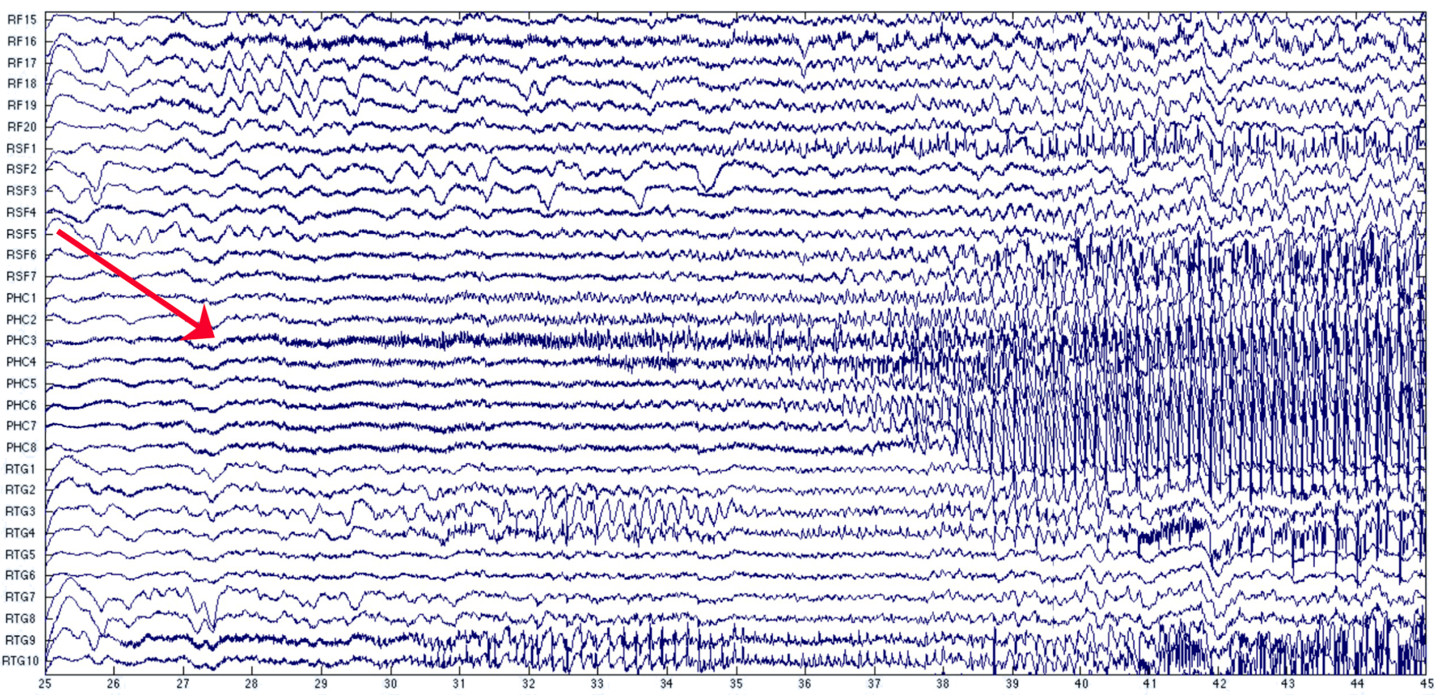
\includegraphics[height =3in]{Plots/Seizure-onset-sample.jpg}
	}
	\caption{IEEG recording of the focal seizure on the representative patient. X-axis represents the time in seconds and y-axis represents the recording sites or electrodes. The arrow shows the electrode contact from where the seizure started. The synchronous activity expanded to other areas in a few seconds.
	\label{fig:seizure-onset-sample}
}
\end{figure*}

\section{Clinical modalities of interest}

\subsection{Intracranial EEG Recording (iEEG)}
Intracranial electroencephalography (iEEG) is a type of invasive electrophysiological monitoring. Most commonly depth electrodes consisting of 1-D linear electrode arrays, shaped in the form of needles, are implanted through cortex into deeper and sub-cortical brain regions. Continuous electrical activities are recorded from these electrodes to capture seizure activities, along with simultaneous video monitoring. Usually, a patient stays in an epilepsy monitoring unit (EMU) for a few days to weeks to record multiple episodes of seizure. The decision for the resection areas are based upon the SOZ identified from these recordings. Figure \ref{fig:structural_scan} shows the positions of implanted depth electrodes in the MRI scan for a representative patient. The red box marks the SOZ as identified from iEEG recording. iEEG provides much better spatial and temporal resolution compared to scalp EEG as these are implanted in the proximity of cortical electrical activity generators. However, the invasiveness of this method can introduce risk of infection, bleeding, strokes and other complications. iEEG can only sample a small area of the brain with a finite number of implanted electrodes. In order to sample the whole brain volume with the present spatial resolution of 3.5mm, about 10,000 recording sites are required \citep{lachaux2003intracranial}. At present, the maximum number of implanted electrodes is a few hundred. Subject to these limitations, there has been growing interest in the combined application of iEEG with non-invasive techniques like functional Magnetic Resonance Imaging (fMRI). 

\begin{figure*}
\centerline{
	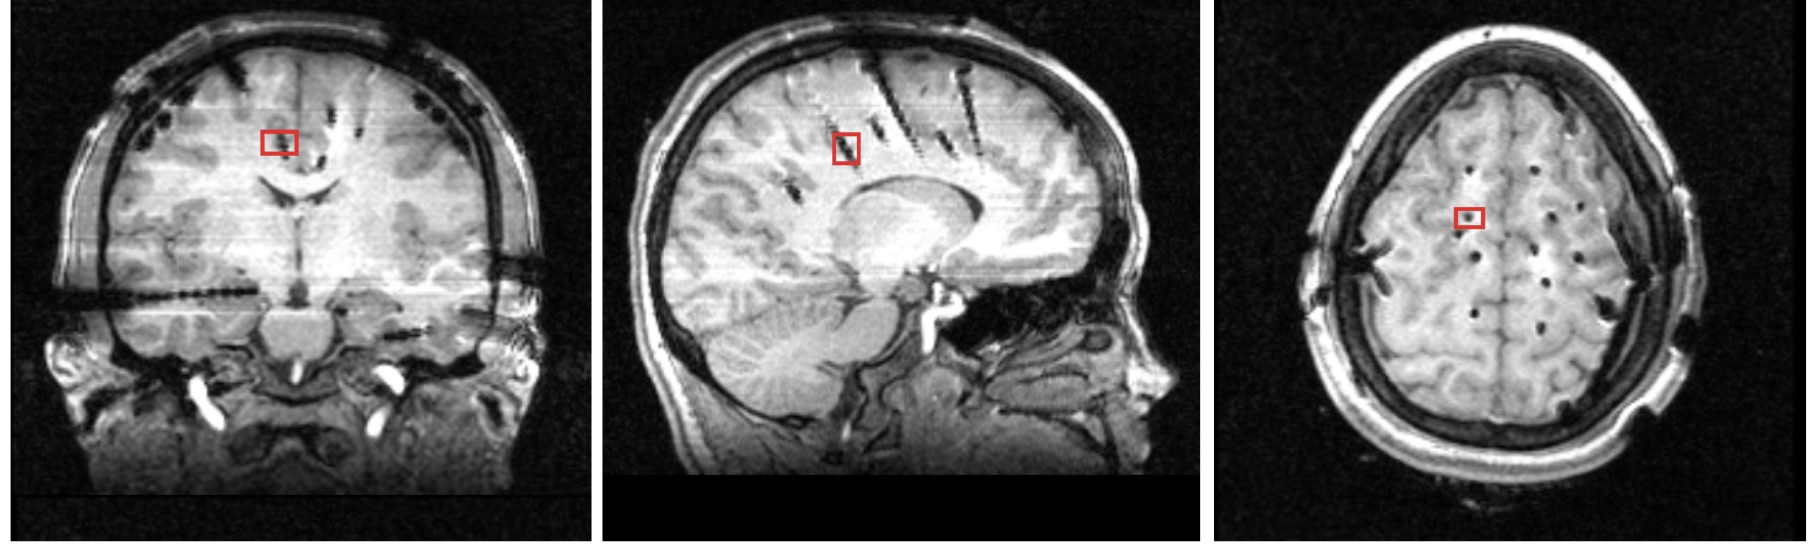
\includegraphics[height =2in]{Plots/Structural scan.jpg}
	}
	\caption{ Magnetic Resonance Imaging (MRI) scan of a patient. An array of electrodes is implanted in the region of the hypothesized SOZ, with 10 contacts for each electrode. The red box highlights the SOZ.
	\label{fig:structural_scan}
}
\end{figure*}


\subsection{Functional Magnetic Resonance Imaging (fMRI)}
Functional Magnetic Resonance Imaging (fMRI) technique is a non-invasive indirect mea- surement of the local neuronal activity which tracks the changes in blood oxygenation over involved brain areas and time. fMRI images are based on the physiological contrast of blood oxygen saturation, thus it is often termed blood-oxygen level dependent (BOLD) signals \citep{ogawa1990oxygenation}. Increased neuronal activity can lead to higher energy demand and vascular changes, which in turn increases the oxygen-rich blood flow and the intensity of recorded BOLD signals \citep{huettel2004functional}. The smallest 3 dimensional smallest unit of these images is called a voxel.

The fMRI signals recorded when the patient is not performing any specific task is called resting state fMRI (rsfMRI). Patients are instructed to lie down with eyes open (or closed), fixated at a screen during collection of fMRI data. The spontaneous low frequency fluctuations ($< 0.1$ Hz) of rsfMRI BOLD signals are utilized to produce surrogate markers for various physiological states and also pathological conditions.

fMRI has been widely used to investigate functional connectivity and large scale network activities in the brain \citep{fox2007spontaneous}. The network between two brain areas or voxels can be studied by a) Seed based correlation maps, b) Spatial independent component analysis of fMRI, or the spatial map of co-varying voxels, and c) Causality analysis between nodes (brain areas) to investigate network dynamics using computation models like dynamic causal models (DCM), structural equation modelling and Granger Causality \citep{centeno2014network}. 

Several research studies have applied these techniques in attempts to localize the SOZ and included prospective patient series, and a few seem rather promising.  However, in general these studies have some pre-defined limitations, identify blobs rather than networks \citep{shah2019characterizing, boerwinkle2017correlating, gil2020beyond, hunyadi2013ica, zhang2015lateralization}, and have not been directly correlated with epilepsy networks as assessed by EEG or other techniques. Fine mapping of spectral (frequency specific) and spatial network from ictal EEG to resting state fMRI could assist in accurate localization of the SOZ, in time and space, further enhancing understanding of the origin and propagation of seizures.
 
\section{Brain oscillations}
iEEG recording consists of frequencies from very low (0.01 Hz) to very high ranges (600 Hz or more). Many studies consider 0.008 Hz to 0.2 Hz as the artifact free useful resting state fMRI BOLD signal \citep{deramus2020modular}. Frequencies higher than 0.2 Hz have been shown to contain useful information in the BOLD signal but can consist of artifacts as well. These broadband frequencies have been observed in different parts of the brain in healthy and neurological conditions. These frequencies are also observed in various task based recordings. 

\subsection{Classical frequencies}
The range from 1 to 80 Hz is sometimes called the classical EEG frequency range, subdivided into frequency bands such as delta (1-3 Hz), theta (4-8 Hz), alpha (8-12 Hz), beta (13-30 Hz, and gamma (30-80 Hz). These classical frequencies have been shown to be associated with different processes like working memory (theta oscillations), alertness, attention and semantic memory (alpha oscillations), cognitive processing (beta oscillations), visual, auditory and motor tasks (gamma oscillations). Few studies have shown coupling of these oscillations with high frequency activities with respect to epilepsy \citep{hashimoto2020coupling, hashimoto2021phase}.

\subsection{High frequency activities}
High frequency oscillations $> 80$ Hz are often subdivided into ripples (80-200 Hz) and fast ripples (200-500 Hz). Two important aspects necessary for recording HFOs are the size of the electrodes and sampling frequency. Recently, commercially available clinical electrodes with specification 4$mm^2$ have been shown to record HFOs in human depth and subdural recording from both temporal and neocortical areas, in both ictal and interictal phases \citep{ochi2007dynamic, worrell2008high, crepon2010mapping, wu2010removing}. The maximum frequency that can be evaluated for HFOs is half of the sampling frequency (Nyquist frequency). Due to the limitations of filters in EEG systems however, the maximum frequency that can be evaluated is about 1/3 of the sampling frequency, requiring at least 240 Hz to record 80 Hz \citep{modur2014high}. HFOs may be generated by inhibitory post-synaptic potentials of the inter-neurons on the pyramidal cells, which are the primary excitation units in human cortex. The fast and synchronous firing of pyramidal cells can be facilitated at a cellular level by neuronal communication methods like axonal sprouting (growth of axons), electrotonic coupling (direct connection between cytosolic contents of adjacent cells), and ephaptic transmission (connection caused by exchange of ions) \citep{jiruska2010electrographic}. HFOs have been associated with both normal and pathologic brain functions. HFOs could play a role in episodic memory and is found to be associated with normal functioning of neocortex. HFOs of hippocampus have been shown to be related to pathologic conditions. Pathologic HFOs have been shown to be helpful in defining epileptic seizure, localizing the SOZ, and identifying propagation pathways in ictal and interictal states \citep{zijlmans2011ictal}. 

\subsection{Infraslow activities}
Infraslow frequencies have been identified variously as - “ultraslow,” “subdelta,” “baseline shifts,” or “near DC” EEG activity in the literature. The upper boundary of recorded activity range from 0.1 Hz \citep{miller2007ictal}, 0.2 Hz \citep{modur2012seizure}, and 0.5 Hz \citep{murai2020scalp} and the lower boundary between 0.01 and DC \citep{kim2009ictal}. In this study, we consider 0.01 to 0.1 Hz as the infra-slow activity (ISA) range. 

There are relatively few studies of ISA in epilepsy. This could be due to past equipment lim- itation of the EEG system with relatively low input impedance and unstable DC baselines over time, and suboptimal electrode/electrolyte interfaces. More recent epilepsy case series argue that widely-available passbands, using conventional EEG systems, are sufficient to provide valuable IsEEG data for visual analysis \citep{rampp2012ictal}. The number of studies is expected to increase with the recent development of wider passbands of the amplifiers, platinum electrodes, and gigaohm input impedances.

The generation of ISA is linked with neuronal and glial activity along with blood brain barrier alteration. The neuronal depolarization during seizure causes an increase in extracellular potassium and glial depolarization. The conduction of this depolarization due to neuron-glial interaction results in negative shifts in deep recording and positive shifts in superficial electrode recordings \citep{shorvon2015treatment}. ISA has been found in many brain regions both in healthy \citep{mitra2015propagated} and pathological conditions \citep{hughes2011infraslow}. 

ISA activities have been observed in qualitative studies before seizure onset \citep{modur2012seizure}, but the quantitative analysis of ISA has been rare. In a recent study by Hashimoto et. al, ripple activities during seizure evolution have been found to be phase amplitude coupled (PAC) with infra-slow (0.016-1Hz) \citep{hashimoto2020coupling} and theta oscillations (4-8 Hz) a few minutes before seizure onset \citep{hashimoto2021phase}. 


%The quantitative analysis of ISA have potential to help in the localization and understanding of seizure origin and propagation.

%None of these studies involved rigorous quantitative analysis of infraslow activity as the basis for a particular choice of frequency range. We applied the main computational tool of this thesis, Granger causal flow, to estimate which portion of this broad range appeared to carry the largest amount of critical information in one subject.

%These preliminary results suggest that the higher frequency ranges suggested by some authors for infraslow might be suboptimal, and further elaboration of our calculations could provide the basis for a more empirical redefinition of the infraslow frequency range.

%Early EEG systems were poorly suited to very low frequency recording, having relatively low input impedance, unstable DC baselines over time, and suboptimal electrode/electrolyte interfaces. Specially designed amplifiers and careful skin preparation were required, but these modifications were feasible only with the relatively small number of channels needed for scalp recording. In the modern era of intracranial EEG recording, where hundreds of contacts and channels may be used, the acquisition of additional special amplifiers in such numbers is financially impractical, and routinely implanting a second set of electrodes virtually impossible. So researchers are practically confined to amplifiers optimized to a higher bandwidth, and to platinum-based electrodes that are biologically inert and compatible with MRI imaging. Manufacturers generally do not provide specifications for the performance of their systems at ISEEG frequencies. However, modern amplifiers generally feature far more stable operation and gigaOhm input impedance.

%Based upon comments from Rampp and Stefan \citep{rampp2012ictal}, and the observation that our own unfiltered EEG data showed very wide variations in DC baselines among different channels (in the range of many millivolts) we used a custom-built ultra low-frequency sine wave generator to directly measure the performance of the Natus amplifiers used for our EEG recordings. Balanced sine wave inputs at wave lengths down to 100 seconds were applied to the inputs. The raw data is shown in Figure \ref{fig:frequency_range}, and the corresponding frequency response curves in Figure \ref{fig:sine-curve-natus-filter-setting}. The colored curves correspond to the Natus filter settings. The X axis displays the frequencies of the input sine waves and the Y axis the measured amplitude of the recorded signal. The three curves to the right, corresponding to digital high pass filter settings of 0.03 - 0.30 Hz, extrapolate to typical single pole high-pass filters with an amplitude rolloff of approximately 10 dB/ decade. The curve corresponding to 0.01 Hz appears to show a milder rolloff. The blue curve, corresponding to the "off" setting of the high pass filter and to the raw data parameters used in all of the analysis for these studies, has an even slower rolloff compared to any conventional analog or digital filter, and may represent simply the inherent limitations of the amplifier outside of its designed performance range. This very slow rolloff and the great interchannel variability of DC baselines support the suspicion that with digital filtering “off,” no conventional high-pass filtering of any kind is being applied to the signal. Above 0.01 Hz amplitude rolloff is less than 10 dB. The high voltages of intracranial ISEEG, measured in hundreds of microvolts, means that this leaves a robust signal for quantitative analysis. However, instrumental phase shift is more difficult to determine.

%\begin{figure*}
%\centerline{
	%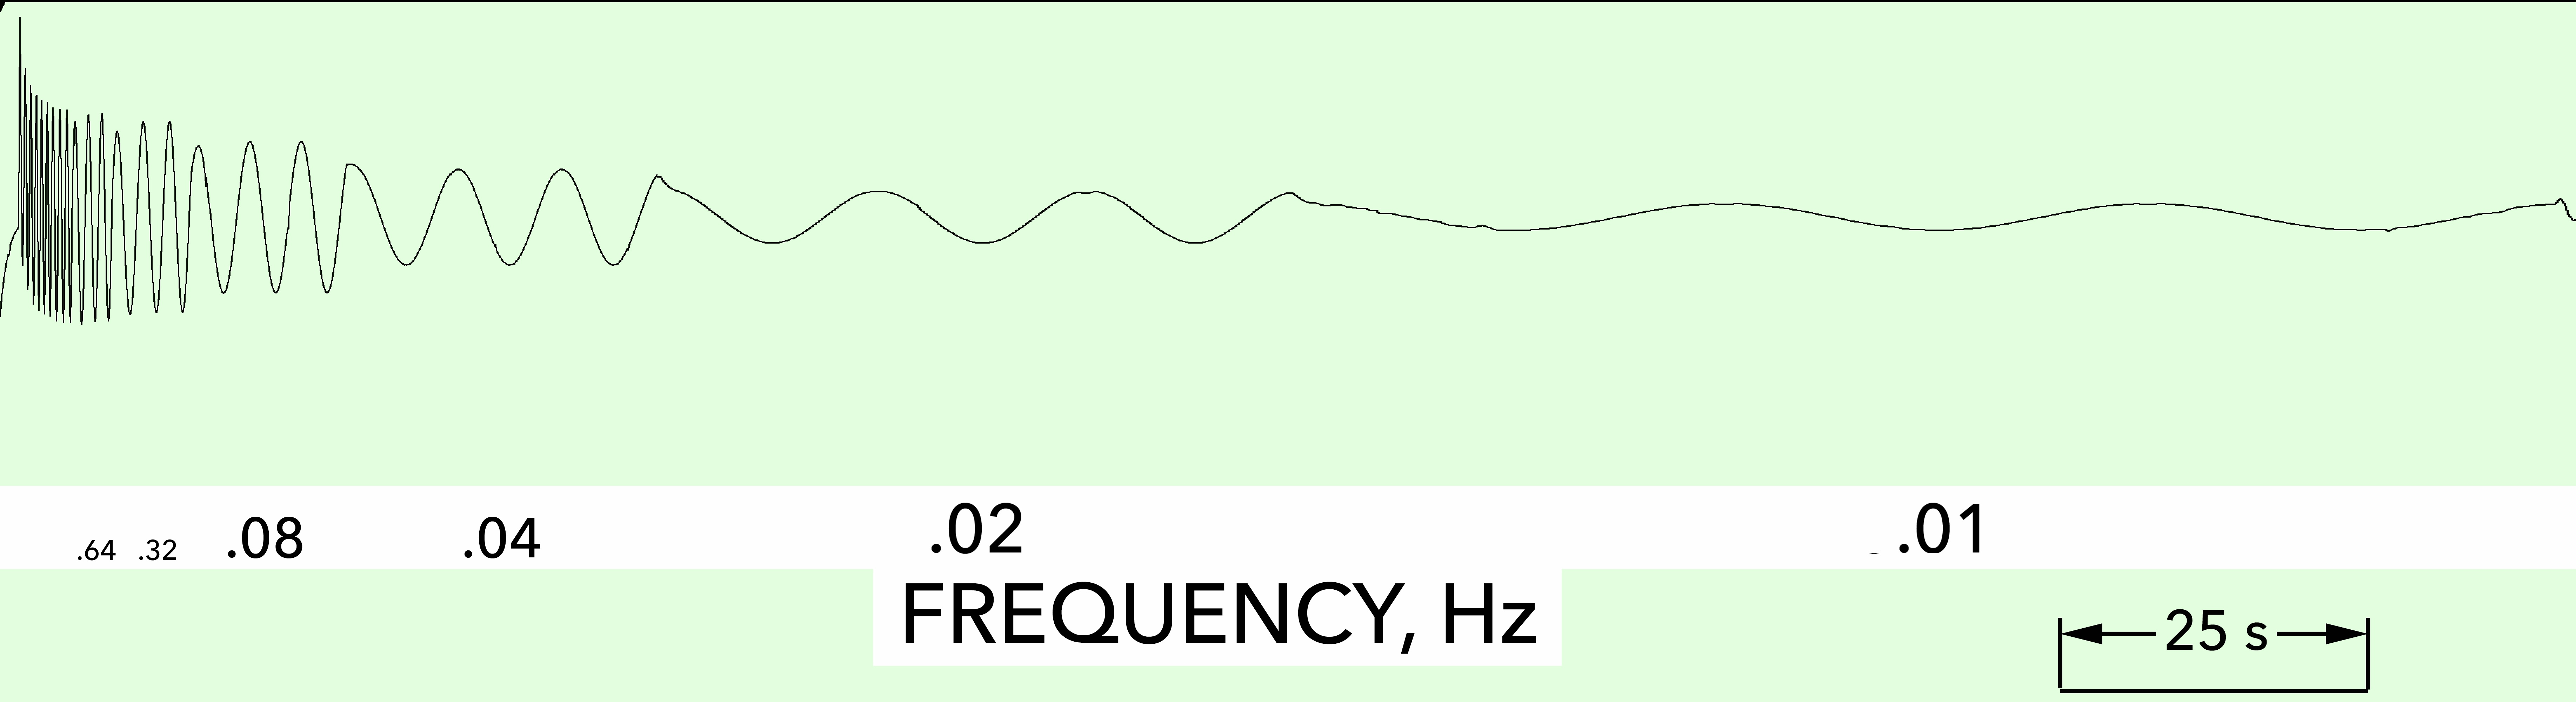
\includegraphics[height %=2in]{Plots/Frequency-range.jpg}
%	}
	%\caption{The full sine wave test curve. Initial offset is due to the custom signal generator, not the recording system 
%	\label{fig:frequency_range}
%}
%\end{figure*}


%\begin{figure*}
%\centerline{
%	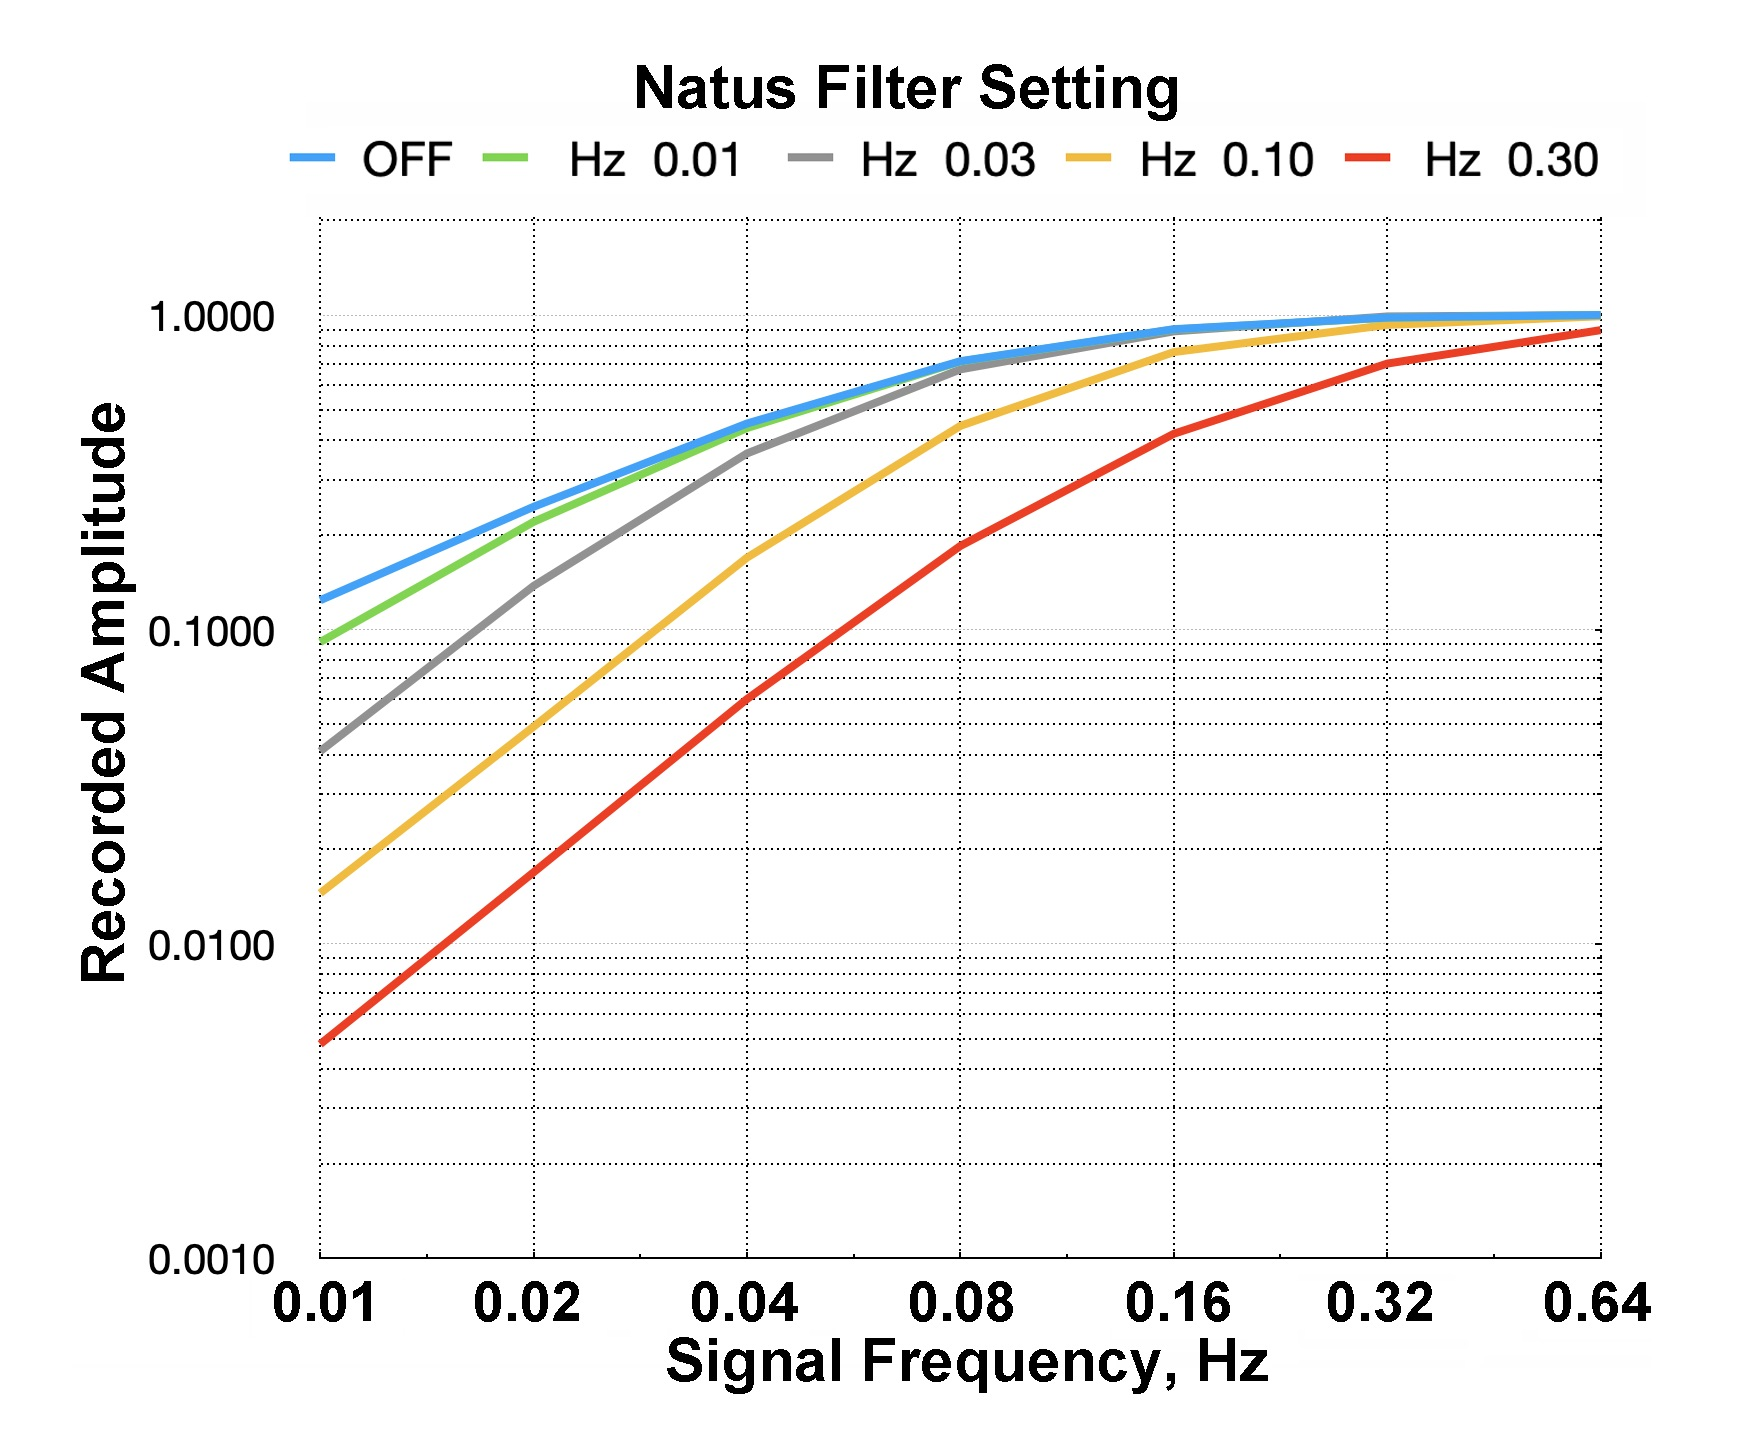
\includegraphics[height %=4in]{Plots/Natus-filter-setting.jpg}
%	}
%	\caption{Frequency response curves derived from the data in Figure \ref{fig:frequency_range}
%	\label{fig:sine-curve-natus-filter-setting}
%}
%\end{figure*}

\section{Quantitative analysis}
Quantitative analysis has been applied to human EEG for well over half a century \citep{grass1938fourier} long preceding the introduction of modern computerized techniques. The study of infra-slow EEG is only a few decades behind \citep{aladjalova1957infra}. However, the early and sustained attention of quantitative studies have been towards higher frequencies rather than the lower. This gap in progression may be due to the technical constraints on the infra-slow recording at the scalp and the arrhythmic nature of the infra-slow EEG as described above. Prior researchers may have assumed that data of this sort was unlikely to carry useful information – especially information that could be extracted by more advanced quantitative techniques.

Recently, there has been an increasing acceptance that a set of distributed regions forms a network during seizure rather than a single focus, thus the recent researchers have applied advanced quantitative methods to model such a system. Many approaches are based on the quantification of the seizure onset zone using a time-frequency analysis of iEEG. 

%Here we review few recent quantitative methods and their application to infra-slow activities, if any.

The linear relationship between iEEG time-series have been estimated using multivariate auto-regressive (MVAR) models in methods like coherence, Granger Causality, direct directed transfer function (dDTF) and partial directed coherence (PDC). The study by \citep{joshi2016regional} have shown strong coherence between electrodes pair 0-2 $cm$  apart in the infra-slow frequency range of ($<0.15 Hz$), but decreased sharply for greater inter-contact distance. DTF methods have been described by \citep{franaszczuk1998application} to determine patterns of flow of activity in pre-ictal periods, whereas \citep{wilke2011graph} discussed the betweenness based on DTF in the classical frequency range for ictal and interictal dataset. \citep{zhang2020establishing} studied graph network derived on partial directed coherence in classical frequency range in both pre-ictal and inter-ictal periods.

\subsection{Granger causality}
Granger causality (GC) is one of the most commonly used methods for determining causal influences (or directional functional connectivity) between dynamical systems by the analysis of their time series measurements \citep{granger1969investigating}. GC is based on the idea of linear prediction by using multivariate autoregressive (MVAR) modeling \citep{wiener1956theory} and uses predictability and statistical dependencies to establish causal relations. GC can be estimated using either autoregressive modeling (parametric methods) or by using direct Fourier or wavelet transforms (non-parametric) spectral decomposition approaches \citep{dhamala2008estimating}, \citep{ding200617}. The definitions and calculation of GC are provided in Appendix \ref{chapter:appendix-definitions}.

Several studies, including from our lab, have successfully utilized Granger causality methods for analysis of high density EEG source waveforms, ICs (independent component) of scalp EEG recording, high frequency activities in preictal, and classical frequencies in in- terictal iEEG \citep{coben2015neural, coito2015dynamic, epstein2014application, park2018granger}. 

\subsection{Graph theory}
A graph is a mathematical structure used to model relations between objects. A graph consists of nodes (vertices) and edges (connection between nodes). Graph theory is the study of graphs (networks), and has been extensively used in numerous studies and applications, including epilogenetic brain network. A graph can be directed, which contains ordered pair of nodes, or undirected, that consists of edges with no specific direction or order. Several graph metrics have been formulated to quantify network characteristics and are widely used in network studies. Some of the commonly used graph measures are Degree and Betweenness. Short descriptions of these measures along with their mathematical definitions are provided in Appendix \ref{chapter:appendix-definitions}.

%Complex dynamical network could be constructed based on the pairwise interactions of iEEG time-series.
Graph theory based techniques have gained interest in the recent years to model the epileptic brain network and find important bio-markers of brain function and dysfunctions. The pairwise interactions of iEEG time-series can be modeled as a graph. Quite a few studies have utilized this method in iEEG signals in preictal, interictal and ictal periods of epilepsy \citep{wilke2011graph, van2013ictal, bartolomei2013interictal, vecchio2016pre}, but none of these include quantitative analysis of infra-slow activities.

\section{Discussion}
Several of the prior qualitative studies and quite a few quantitative studies on infra-slow iEEG have shown promising results for the usefulness of these signals in extracting important biomarkers in an epileptic network. However, to the best of our knowledge, there is no comprehensive study that quantifies the infraslow network and examines its correlation with high frequency activities throughout all stages of focal epilepsy. Chapter \ref{chapter:ieeg-infraslow-hfo-correlation} of this dissertation presents such study where we examine the correlation between the two dfferent frequency ranges throughout all epilepsy stages.
One of the other unexplored areas is the concordance between infraslow iEEG and resting state fMRI and if are able to seed epilepsy network from iEEG to rsfMRI for finer focus localization, which is discussed in Chapter \ref{chapter-seeding-iEEG-to-fmri}.
%!TEX root = ../main.tex

\chapter{Functional Connectivity Correlation between Infraslow and High Frequency iEEG Activities}
\label{chapter:ieeg-infraslow-hfo-correlation}

This chapter examines the concordance between infraslow ($<0.1$) and high frequency ($>50$ Hz) iEEG neural information flow throughout multiple phases of epilepsy using Granger causality and graph theory. Results on three epileptic patients show overlap in the epileptic network as observed in the high to infraslow, and from preictal to the interictal, to the visible ictus.

\section{Introduction}

Few studies have shown that infraslow EEG (IsEEG) could be used as an ancillary tool for the localization of the seizure focus in scalp 
\citep{leistner2007combined, miller2007ictal, murai2020scalp}.
Several groups have also studied the relationships among IsEEG, the classic EEG frequencies, and the gamma or higher frequency ranges 
\citep{modur2012seizure, wu2014role, thompson2016interictal, inoue2019interictal}. But the utility of very low-frequency recording in epilepsy has not been universally accepted \citep{gross1999intracranial}. Only a fraction of publications concerning IsEEG and epilepsy have employed any form of quantitative analysis \citep{modur2012seizure, thompson2016interictal, thompson2016ictal, murai2020scalp}, and none appear to have applied it to HFO and infraslow EEG on the same patient.

In several prior studies in our lab, Granger causality (GC) \citep{granger1969investigating} has been used as an analysis tool for intracranial EEG (iEEG) in the high frequency bands, and found widespread network activity prior to visible seizure onset \citep{adhikari2013localizing, epstein2014application}. 

In this study, we apply Granger causality (GC) and connectivity analysis to high frequency and infraslow activities throughout multiple phases of focal epilepsy, from preictal to interictal. Results show a striking consistency among the iEEG networks identified by GC at both high and IsEEG frequencies, along with the visual seizure onset; plus the persistence of this network during the pre-ictal, and interictal phases of epilepsy.  

\section{Materials and methods}
\label{sec:methods}

\subsection{Patients selection}
All the data were analyzed under protocols approved by the Institutional Review Board of the Emory University School of Medicine. Patients - A, B and C were chosen retrospectively based upon meeting the following criteria: an established history of medication-refractory epilepsy, absence of obvious anatomical lesion on 3 Tesla MRI, clinical confidence in the site of seizure onset by contemporary intracranial EEG (iEEG) features and ancillary studies, and long-term improvement in clinical seizures following a focal invasive procedure. Additional data included positron emission tomography (PET), neuropsychological assessment, and if indicated, single photon emission computed tomography (SPECT), magnetoencephalography (MEG) or functional MRI (fMRI) mapping. All three patients had striking improvement (1) or prolonged remission (2) following invasive procedures.

Patient A had no known clinical seizures following bilateral mesial temporal electrode explantation, or for 18 months afterwards. Over the subsequent 6 years, seizures have been substantially milder and rarer than before the implantation. Prior to selection for the current investigation, this case had been assessed as a rare instance of long term remission related to implantation of intracranial electrodes \citep{katariwala2001remission, schulze2010seizure} . The striking and prolonged clinical improvement was considered strong confirmatory evidence for seizure origin at the site of implantation.% Patient B is GA

Patient B elected responsive neural stimulation following recording of electrographic seizure onset at a site where tissue ablation was considered to have high risk of permanent neurological deficit; this has resulted in sustained reduction in symptomatic seizures for  years.
% Patient C is QM

Patient C  has been in complete remission (Engel 1A)
for 4 years following laser ablation along the track of the electrode that recorded electrographic seizure onset 
% Patient A is WD


\subsection{IEEG recording}
Patients underwent implantation of depth electrodes, subdural grids, and/or strip electrodes (Ad-Tech Medical, Racine, USA) in various combinations according to the individual pre-surgical localization hypothesis.  Recordings were made with an XLTEK system (Natus Medical, San Carlos, CA, USA) using up to 128 electrodes. 

\begin{figure*}
\centerline{
	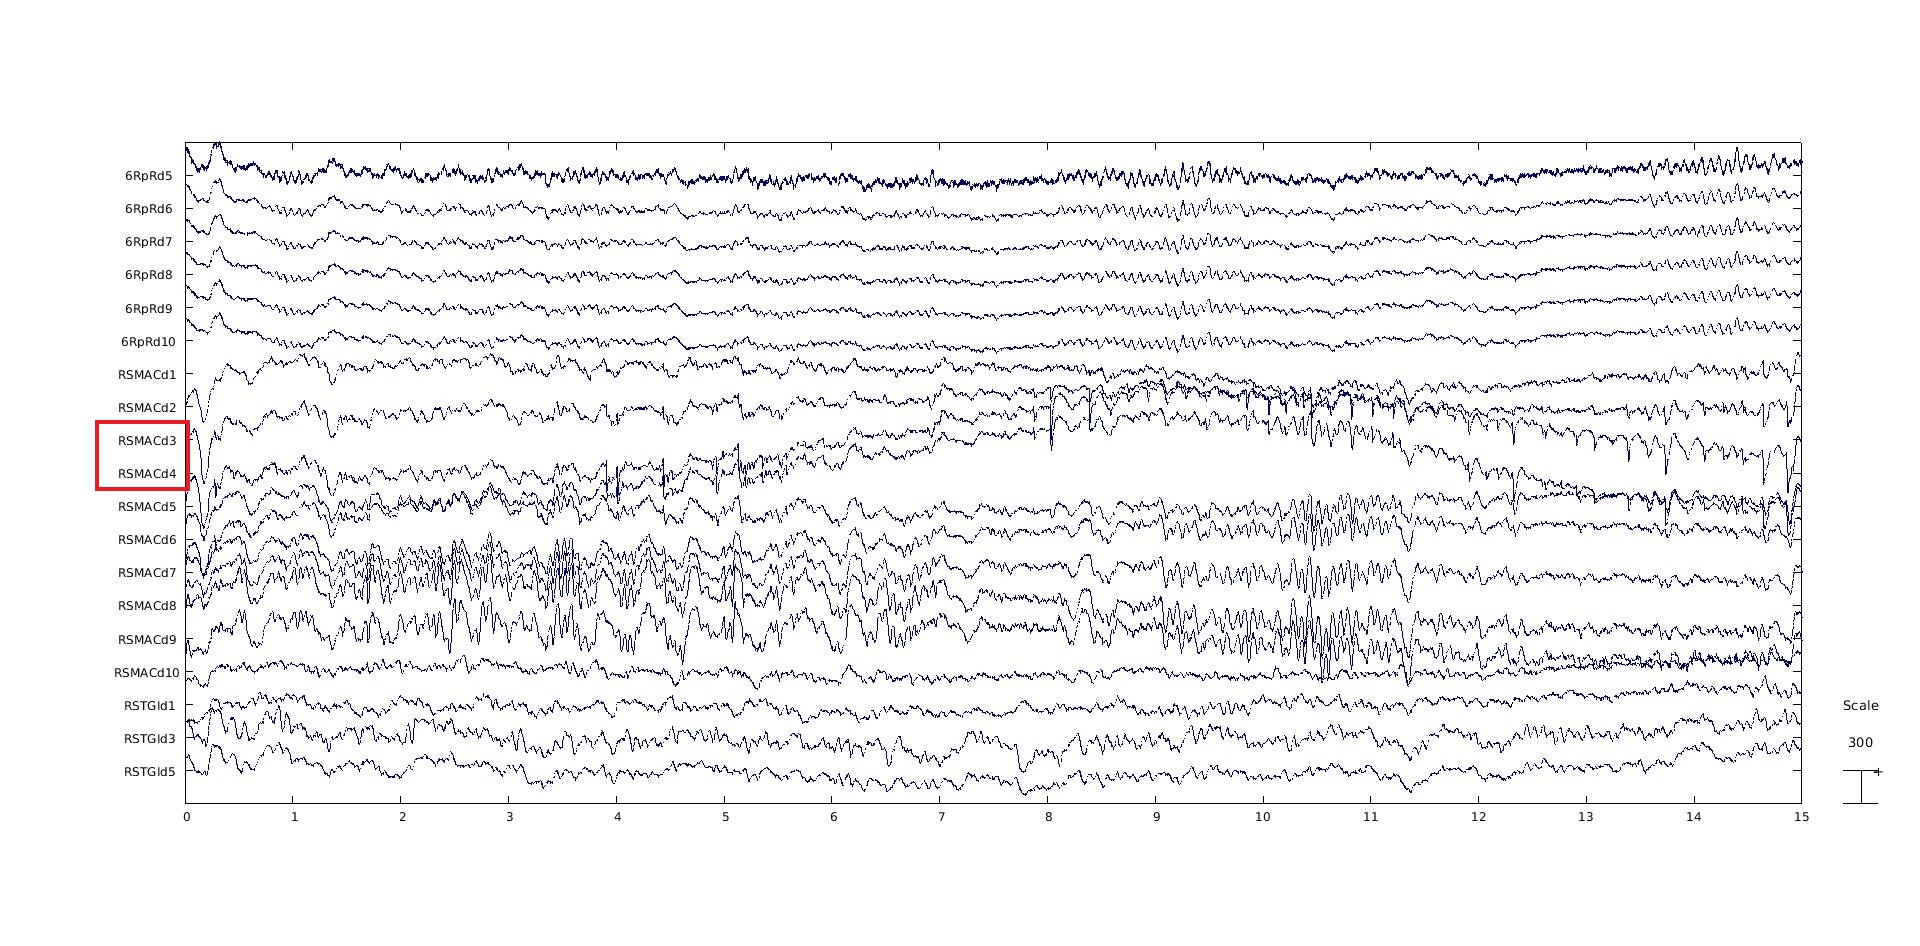
\includegraphics[height = 3.5in]{Plots/Patient_C_iEEG_rawdata_sample.jpg}
	}
	\caption{The unfiltered iEEG time-series shows spikes riding on top of slower waves on seizure onset electrodes in pre-ictal and ictal period. The red box highlights the seizure onset (SO) electrode.}
	\label{fig:rawdata_patient_c}
\end{figure*}

Initial oversampling and hardware antialiasing filters were followed by linear phase FIR filters with an order of 30, set to just below the Nyquist frequency for the final sampling rate of 500 or 1000 Hz. The Natus digital preamplifiers were specified to a lower frequency limit of 0.01 Hz, but no filtering was applied during download of wideband European Data Format (EDF) data for analysis. Visual identification of the iEEG seizure focus was performed according to current criteria \citep{andrzejak2015localization,grinenko2018fingerprint,gnatkovsky2019two} and the results of invasive therapies or procedures. Figure \ref{fig:rawdata_patient_c} shows the IEEG time-series on a few electrodes including the SO electrodes on a representative patient. The spikes are on top of slow waves. Similar infra-slow wave patterns relevant to seizure onset electrodes have been reported in \citep{rampp2012ictal}.



\subsection{Data pre-processing}
The iEEG time-series data were filtered using forward and backward finite impulse filters (FIR) in EEGLAB \citep{delorme2004eeglab} for its simple design, intrinsic stability and free of phase distortion. The data were band-pass filtered at a cutoff of 50 Hz to Nyquist frequency (half of the sampling frequency) for high frequency oscillations (HFOs) analysis and cutoff for infra-slow oscillations (ISO) were 0.01 Hz and 0.1 Hz. Temporal mean was removed from the time-series before advanced mathematical calculations. Pre-ictal data samples for high frequency activity were taken for 64, 69, and 54 seconds ending 1-2 seconds before visible seizure onset for patients A, B and C. Variable length of data segments were considered for different patients due to the artifacts present in the data. Similarly, 1550, 113 and 330 seconds data samples were analyzed for inter-ictal iEEG recording. For low frequency activity, data samples were selected visually to correspond to the beginning and the end of a baseline shift that coincided or overlapped with the visible seizure onset and was congruent with it in multiple electrodes.

\subsection{Time frequency analysis}
The wavelet based spectral power was computed from unfiltered iEEG time-series to investigate when and how the power changes for high frequency oscillations and infra slow oscillations in the seizure onset electrodes. We did not study the wavelet power for all the electrodes, for pre-ictal and interictal periods separately, as previously done in \citep{adhikari2013localizing} for high frequency oscillations. The aim of time frequency analysis is to confirm the significant high and infraslow oscillations in these iEEG time-series. This facilitates meaningful quantitative spectral interdependency analysis.

\subsection{Granger causality}
We computed pairwise Granger causality spectra and graph measures, as directed functional connectivity matrices to examine the strengths and directions of causal interactions in the frequency domain, among multi-channel digitized iEEG time-series \citep{dhamala2008analyzing}. Granger causality as computed in the time domain is the statistical technique that relies on the concept of temporal precedence of cause before effect and is based on the prediction of future behaviors using the past records \citep{granger1969investigating}. If the past of one time series X1 can help predict another time series X2 better than using the past of X2 alone, then X1 is known to have a causal influence on X2. Due to the difficulty of finding an optimal model order in the parametric pairwise approach, we used both non-parametric and parametric approaches at different model orders and selected the model order that yielded the lowest power difference. Accordingly, we obtained the optimum model order 8 for our analyses. Time domain Granger causality was obtained by integrating in the infra-slow frequency range and high frequency range as specified above.
%We would consider this method helpful in SOZ prediction if the leading visual electrodes and the strongest high-frequency and low frequency electrodes are identical.

\subsection{Graph measures}
Graph measures were computed from the time domain Granger causality matrix as the adjacency matrix using the BCT toolbox \citep{rubinov2010complex} with a threshold of 40\% above the maximum Granger causal flow. The electrodes were considered as the nodes and the causal relations between nodes were considered as the edges. Three centrality measures, betweenness, degree and closeness were computed to study the importance of SO electrodes in the network. Betweenness measure was computed for all the high-frequency and infraslow GC spectra from preictal to ictal period to study the number of paths SO electrode lies in the network graph. This represents the SO electrode's ability to make connections to other groups of brain areas \citep{chiang2014graph,wang2008betweenness}
Likewise, ‘Degree’ measures the number of edges of a node, and nodes with higher edges act like a hub of activity. Closeness centrality is the inverse of the sum of all shortest paths to other nodes. A higher closeness value corresponds to faster information spread throughout the network. For directed graphs, the closeness value is called ‘Incloseness’. Clustering coefficient is the measure of segregation of the network.


\section{Results}
\label{sec:results}

\subsection{Time frequency analysis}
We focused our study on high frequency oscillations and infra-slow oscillations in preictal and interictal periods. Figure \ref{fig:high_pass_filtered_preictal_patient_c} provides a sample iEEG time series after finite impulse filtering (FIR) for high frequency oscillations. This data includes clinically identified seizure events illustrating HFOs as one of the biomarkers of seizure onset electrodes. Even though HFOs were observed in all channels in both preictal and interictal states, the evolution of HFOs was distinctly visible in the SO electrode and later extended to multiple channels, mostly in preictal period.

Figure \ref{fig:infraslow_wave_patient_c} represents 100s of infraslow activities in a representative patient, which illustrates infraslow activity not just before seizure onset but during the interictal period as well. Infraslow activities were observed in a few other channels, including SO electrodes, in both these periods in all patients. This motivated us to further quantitative analyses of these activities to determine if infraslow activities during the interictal period correlates with the SOZ.

The complex wavelet transform performed on these filtered iEEG time-series depicted distinct maximum wavelet power for high frequency in the 50 Hz to 120 Hz, as shown in Figure \ref{fig:power_plot}(a). Time frequency analysis of infraslow activity was observed around 0.03 Hz for SO electrodes of same patient as shown Figure \ref{fig:power_plot}(b). Maximum power was observed in different frequency ranges for other electrodes both in high and infraslow analysis. The time frequency spectral analysis results for all the channels are not discussed in this paper as our goal here is to demonstrate the presence of high and low frequency components in our iEEG data for further quantitative analysis.


\begin{figure*}

\centerline{
	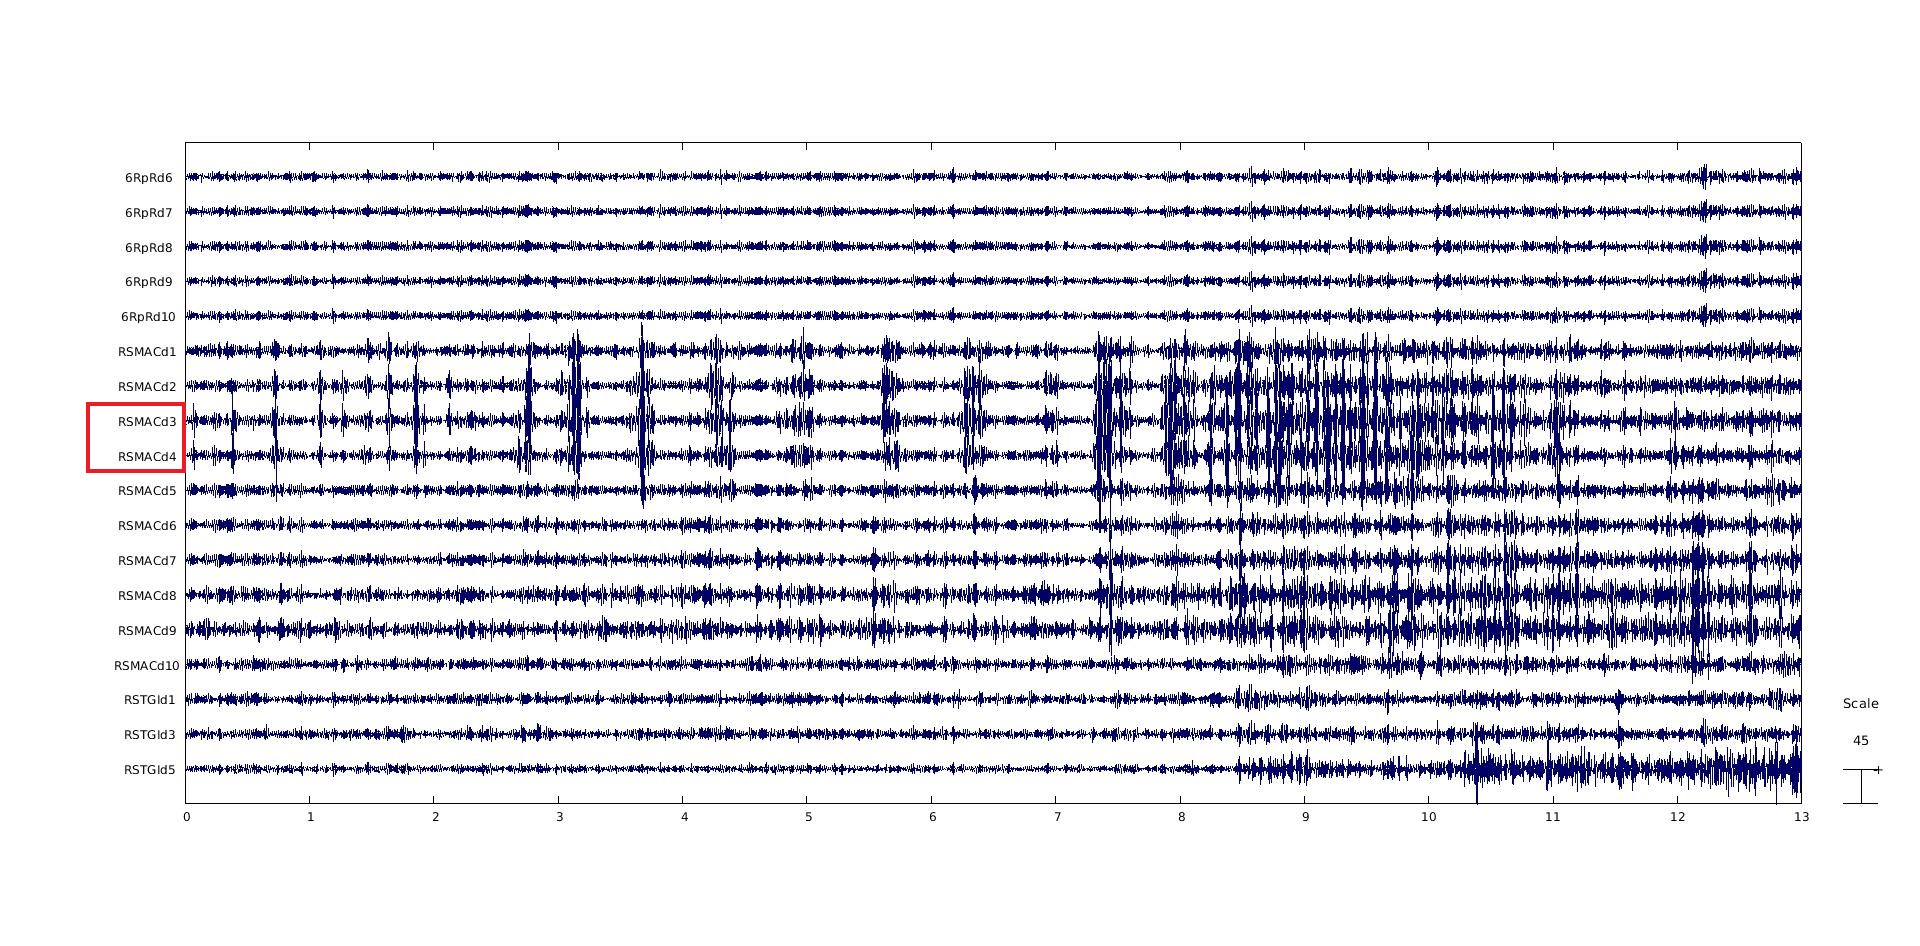
\includegraphics[height =3.5in]{Plots/Patient_C_HFO_Filtered.jpg}
	}
	\caption{13s high pass filtered iEEG time-series. High frequency activities ($> 50 Hz$ to Nyquist frequency) are visible on seizure onset electrodes RSMAcd3 and RSMAcd4 and later extended to other electrodes.}
	\label{fig:high_pass_filtered_preictal_patient_c}
\end{figure*}


\begin{figure*}
\centerline{
	\includegraphics[height =3in]{Plots/Patient_C_infraslow_100s.jpg}
	}
	\caption{100s low pass filtered iEEG time series (0.01-0.1 Hz). Infraslow activity is visible in SO electrode RSMAcd4.}
	\label{fig:infraslow_wave_patient_c}
\end{figure*}



\begin{figure}%
    \centering
    [\centering a]{{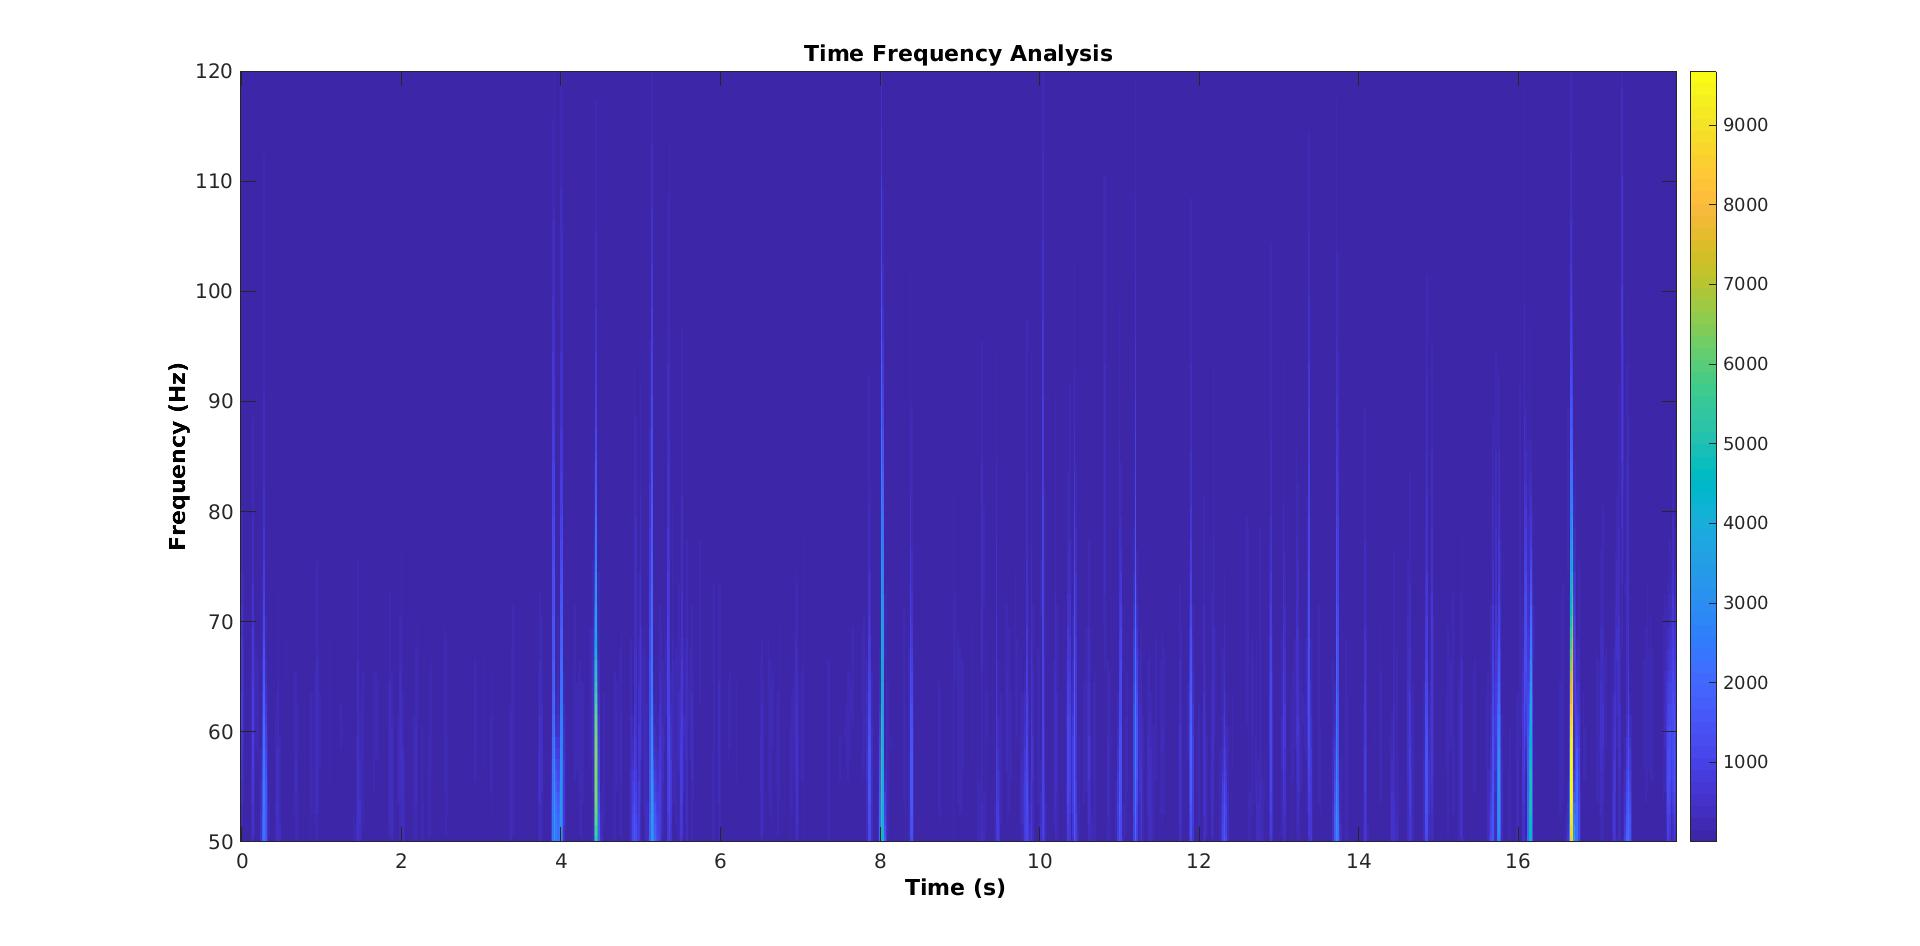
\includegraphics[width=15cm]{Plots/Time_Frequency_HFO_RSMAcd4.jpg} }}%
    \qquad
    [\centering b]{{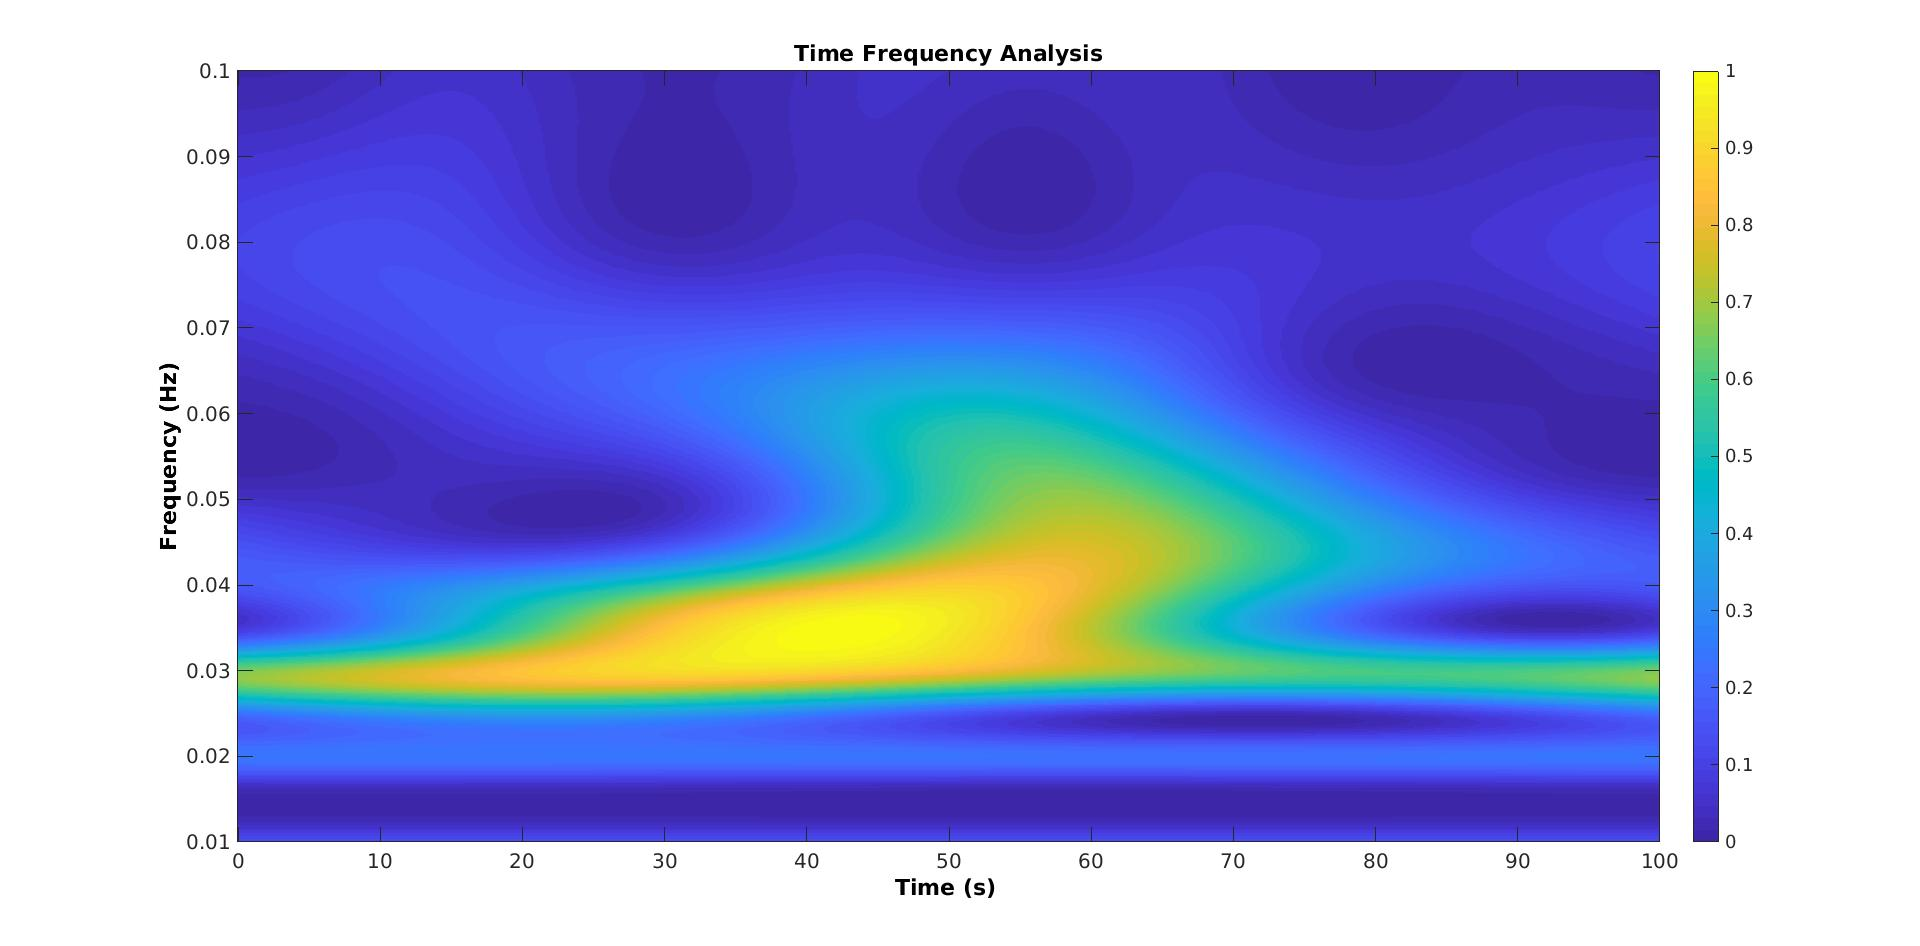
\includegraphics[width=15cm]{Plots/RSMAcd4_powerplot_infraslow_interictal.jpg} }}%
    \caption{High frequency activities as observed in representative patient on SO electrode, RSMAcd4. Scattered blobs of high frequency activity could be seen from 50 Hz-100 Hz. Time frequency analysis was done on iEEG time-series a few seconds before clinical seizure onset b) Wavelet power was computed on 100s iEEG time-series hours away from any seizure activity (inter-ictal state) for SO electrode RSMAcd4. The power was normalized between 0 and 1. Wavelet power was maximum between 10s and 70s and in the frequency range of 0.03 Hz and 0.05 Hz.}%
    \label{fig:power_plot}%
\end{figure}



\subsection{Granger causality and graph measures}
We studied characteristics of high frequency and infra-slow oscillations by computing GC spectra, source, sink and total causal flow. Neuronal information flow from the electrode to all other electrodes is called outflow or source. Similarly, neuronal information flow from all other electrodes to this electrode is termed inflow or sink activity. Total Granger causality is the sum of inflow and outflow. 

%High frequency oscillations
These measures were computed from high pass filtered iEEG time series above 50Hz to just below the Nyquist frequency with a frequency resolution of 1 Hz for HFO analysis. 
%Temporal mean was removed from the data prior to GC calculations

Figure \ref{fig:patient_c_preictal_high} shows the GC (sink and total GC) for HFOs in preictal period for a representative patient. Sink activities are visualized in the negative axis to represent incoming neuronal information flow. Red circles in the figure, denoting SO electrodes as confirmed visually by the epileptologists, were ranked in the top 5, out of 119 electrodes for causal Sink measures. Blue circles denote the contralateral SO electrode, which interestingly are also ranked among the topmost values for total GC only. We were able to localize SO electrodes for patients A, B and C (Shown in Appendix \ref{chapter:appendix-gc-results}) using these tools and methods. Sink and total GC were also clustered around SO electrodes for these patients. 

%Infraslow oscillations
Similarly, infraslow oscillations were quantified from low pass filtered iEEG time series in the frequency range 0.01 to 0.1 Hz with 1/1000 frequency resolution. Figure \ref{fig:patient_c_interictal_low} show the integrated time domain Granger causality, Sink and Total GC computed and integrated over infraslow frequency in interictal periods for the same patient. Total GC and sink activities were highly clustered around SO electrodes for this representative patient as well as two other patients (Shown in Appendix \ref{chapter:appendix-gc-results}). SO electrodes were ranked $2^{nd}$ out of 119 electrodes for both Sink and Total GC.


% \begin{figure*}
% \centerline{
% 	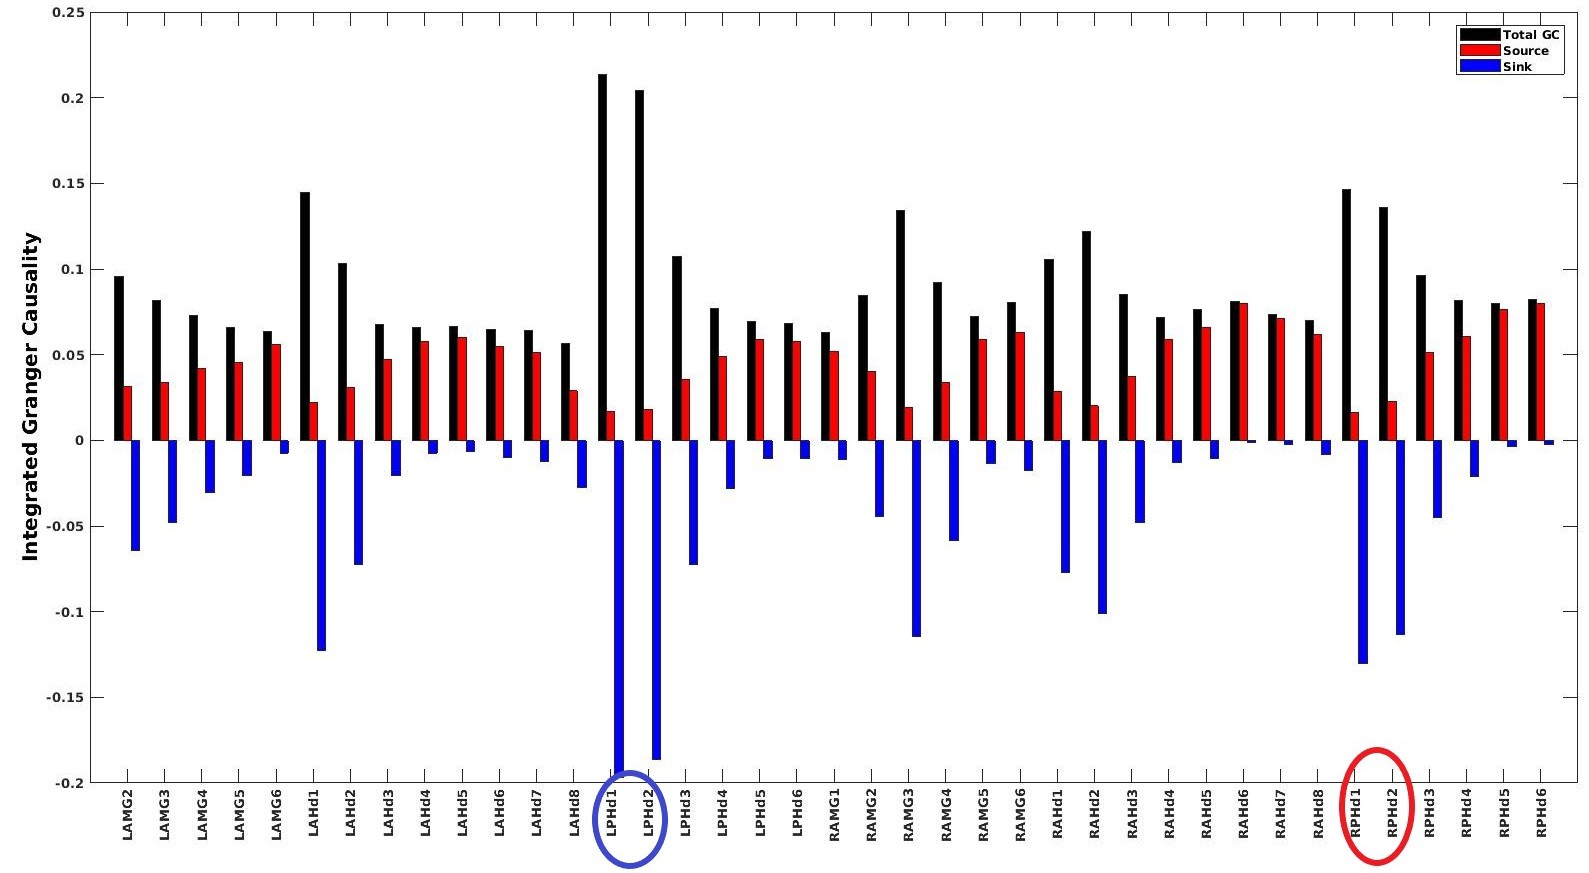
\includegraphics[height =3.5in]{Plots/Patient_A_preictal_high.jpg}
% 	}

% 	\caption{Integrated Granger Causality for preictal states for patient A. Source, sink and total were computed for 40 implanted electrodes. RpHd1 and RpHd2 are the SO electrodes on the right hemispheres. LpHd1 and LpHd2 are the contralateral electrodes. Both total GC and sink activities were maximum for contralateral electrodes and RpHd1 and RpHd2 were also ranked among the top for both total GC and sink. Source activity could not explain much about the seizure activity}

% 	\label{fig:patient_a_preictal_high}
% \end{figure*}


% \begin{figure*}
% \centerline{
% 	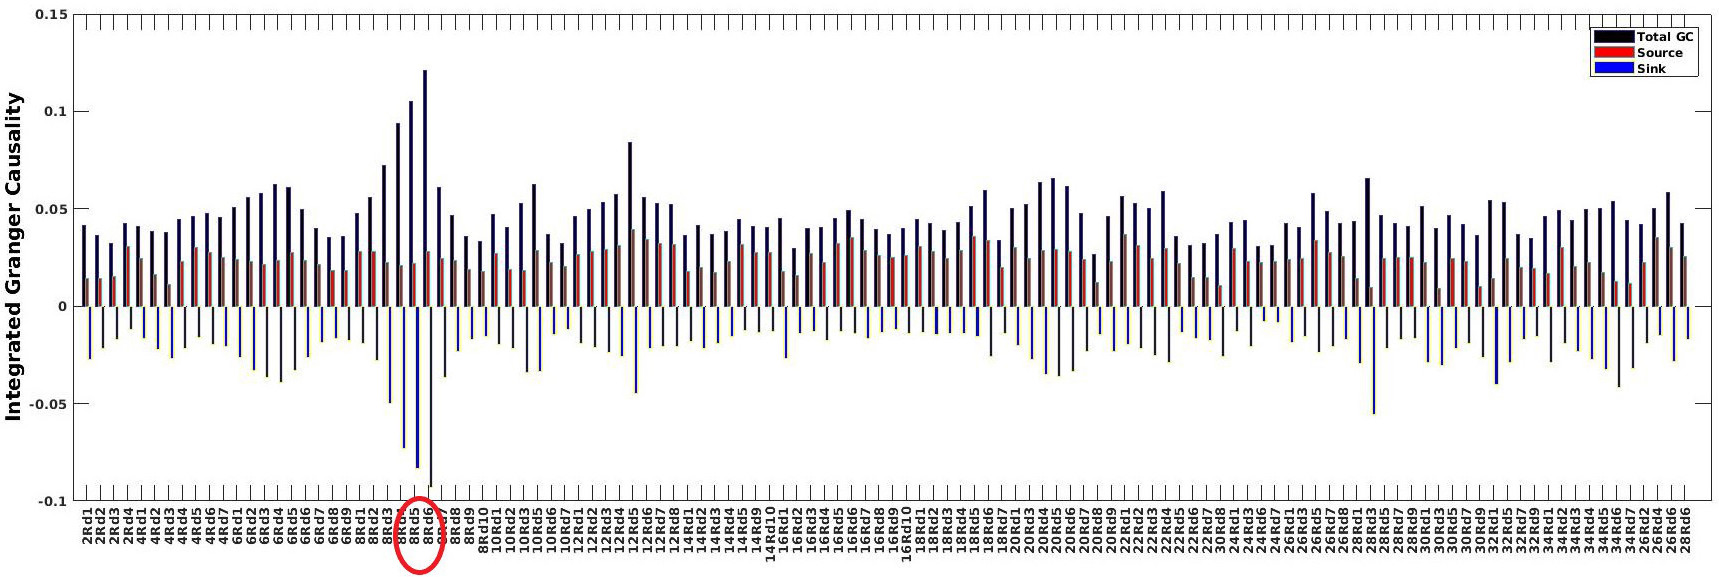
\includegraphics[height =3in]{Plots/Patient_B_preictal_high.jpg}
% 	}

% 	\caption{Integrated Granger Causality for patient B. SO electrodes 8Rd5 and 8Rd6 have very high total GC and sink measures value, suggesting that these two measures could be used for SO electrodes prediction for prospective patients}

% 	\label{fig:patient_b_preictal_high}
% \end{figure*}

\begin{sidewaysfigure*}
\centerline{
	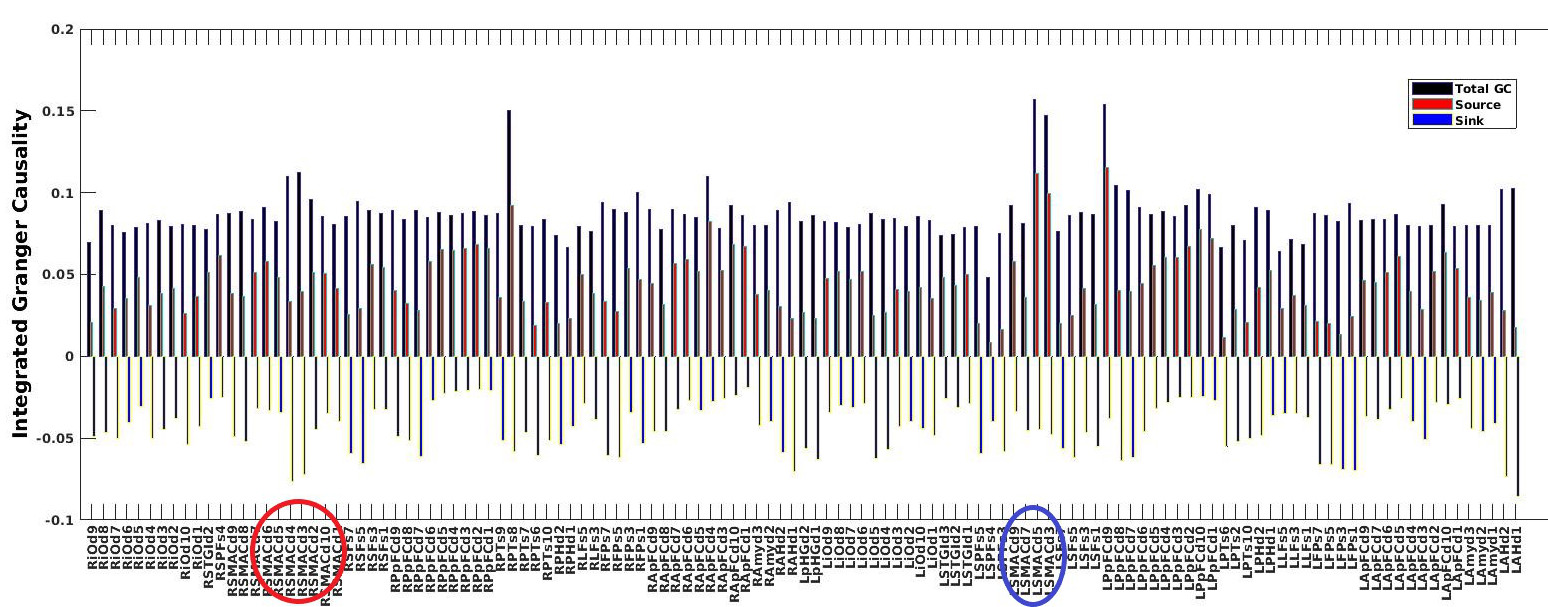
\includegraphics[height =3in]{Plots/Patient_C_preictal_high.jpg}
	}

	\caption{Integrated Granger causality of high frequency activities in preictal state for a representative patient. The SO electrodes RSMAcd are second and forth from the top for causal sink activity. The contralateral channel LSMAcd was ranked highest for Total GC.}

	\label{fig:patient_c_preictal_high}
\end{sidewaysfigure*}


\begin{sidewaysfigure*}
\centerline{
	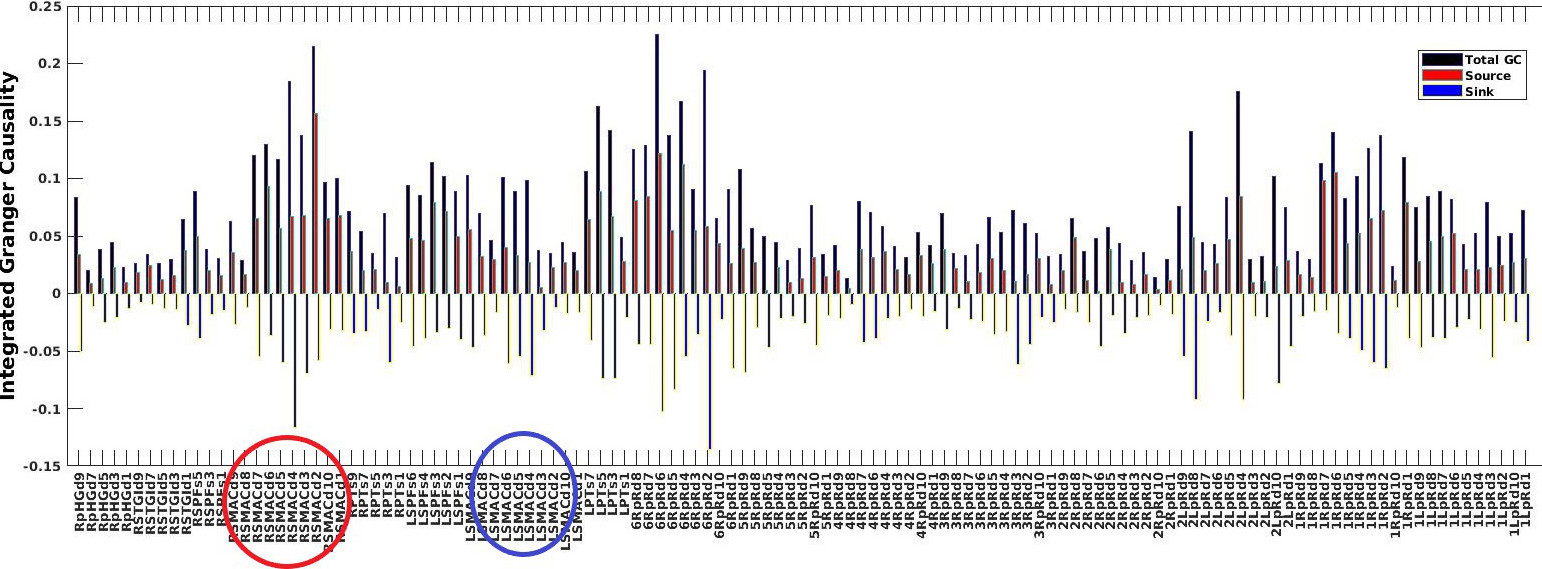
\includegraphics[height =3in]{Plots/Patient_C_interictal_low.jpg}
	}

	\caption{Integrated Granger causality of infraslow activities in the interictal state for a representative patient. The SO electrodes RSMAcd3 and RSMAcd4 are ranked at the top 2 out of 119 electrodes based upon Total GC and Sink measures. Contralateral electrodes LSMAcd3 and LSMAcd4 are much less prominent for this frequency range and state.}
	\label{fig:patient_c_interictal_low}
\end{sidewaysfigure*}

The threshold value of each integrated GC measure, for statistical significance, was computed from surrogate data methods by using data permutation calculating GC values and a gamma function fit to a distribution of maximum GC values for each permutation. This threshold was designed to reject a null hypothesis of no interdependence at a significance level of $p <10^{-6}$ as in \citep{adhikari2013localizing}.

To validate and compare the Granger causal measures, we also computed the graph theoretical measures - degree, betwenness and clustering coefficient and incloseness. Table \ref{table:summary} provides a summary view of the effectiveness of these measures along with the causal measures (Total GC and ) in localizing the seizure onset for both high and infraslow oscillations in the preictal and interictal periods. If for a particular patient, the SO electrode belongs among the top 5 for a given measure, it is considered as correct localization and counted 1, otherwise it is counted 0. Thus, the values in this table represent the number of patients for which the measure is able to localize SOZ.

As observed in the table, using the total Granger casuality, the SO electrodes were localized appropriately in all the patients for HFO in the preictal and infraslow in the interictal period. Likewise, sink and betweenness measures could predict the SO electrodes in preictal periods for high frequency only. These results suggest that either total or negative causal flow (sink), or betweenness measures could correlate seizure focus in different patients and different phases of epilepsy cycle in both high and infraslow frequency.



\begin{table}[]
\renewcommand{\arraystretch}{1.2} % Default value: 1
\setlength{\tabcolsep}{12pt} % Default value: 6pt
\centering
	\begin{tabular}{|l |c|c|c|c|}
	\hline
	  & \multicolumn{2}{c|}{\textbf{High}} & \multicolumn{2}{c|}{\textbf{Infraslow}} \\ \cline{2-5}
	\multirow{-2}{*}{\textbf{Measures}} & Preictal        & Interictal       & Preictal       & Interictal       \\ 
	\hline
	\textbf{Total GC}                   & 3               & 2                & 2              & 3                \\ \hline
	\textbf{Sink}                       & 3               & 2                & 1              & 2                \\ \hline
	\textbf{Betweenness}                & 3               & 2                & 1              & 1                \\ \hline
	\textbf{Degree}                     & 2               & 2                & 2              & 2                \\ \hline
	\textbf{Clustering coef}            & 0               & 1                & 0              & 1                \\ \hline
	\textbf{Incloseness}                & 1               & 0                & 2              & 1                \\ \hline
	\end{tabular}

	\caption{Summary listing the no. of patients for which corresponding causal and graph measures are able to localize the SO electrodes across preictal and interictal periods, in high frequency and infraslow oscillations}
	\label{table:summary}
\end{table}


\section{Discussion}
\label{sec:discussion}
In this work, we confirmed the existence of a stable iEEG network in very low to very high frequencies throughout multiple phases of focal epilepsy, from preictal to interictal, to visible ictus, using quantitative analysis methods based on spectral interdependency measures including GC spectra computation and graph measures. These network features were identified from among large sets of iEEG electrodes in selected patients who experienced sustained remission following focal invasive procedures and lacked obvious anatomic lesions. In addition to the seizure-onset patterns on iEEG, remission confirmed the accuracy of seizure localization.  Absence of anatomic lesions helps exclude the alternative possibility that focal changes in infraslow activity might be due simply to the lesion rather than to the presence of an epileptic focus.

The statistical connectivity results of integrated GC and graph measures suggested the extensive spatial-temporal neurophysiological network and its relationship to the site of focal seizure onsets both in the infra-slow frequency (0.01-0.1 Hz) and the high frequency ($> 50 Hz$ to Nyquist frequency).  Although the amplifiers in digital EEG recording equipment may lack the specific characteristics considered desirable for true DC recording, no fixed high pass filter appeared to be present, and activity below 0.1 Hz was quantified through methods of frequency analysis. 

Both sink and total GC activity were ranked among the top for all three patients for HFOs, but for infraslow activity, only total GC could localize SO electrodes, mostly in interictal periods. This could be explained on the hypothesis that during the preictal period, seizure onset zone is subject both the uncontrolled hyperactivity and increased external inhibition, which may fluctuate over time scales much briefer than this analysis., and produce maximum sink activities in these electrodes. This has been illustrated  in \citep{epstein2014application}. For interictal infraslow activity, the time duration of the measured signal is orders of magnitude is orders of magnitude slower than the feedback loops of much neuronal activity, so that infraslow measures would show only net effects. Our results suggest that total causal flow (sum of source and sink) could be higher for these nodes in interictal periods. Other groups have reported sink activity, but not that it could be either that or total \citep{narasimhan2020seizure}. The graph measures for corresponding periods could be explained on a similar hypothesis, as these were derived from the GC connectivity matrix. 

%This activity identifies the location of the epileptic seizure focus within the human brain both immediately prior to the visible seizure onset (preictal) and remotely (interictally), many hours from any visible seizure. 

The methods and results discussed in this study do not test the utility of infraslow iEEG in predicting surgical outcomes. However, they supplement the findings of larger surgical series \citep{narasimhan2020seizure, david2011imaging}, which indicate that interictal EEG networks may contribute valuable information to the epilepsy surgery assessment, thereby substantially reducing the time, risk, and cost of diagnostic pre-surgical testing. Given the relatively high voltages intrinsic to infraslow iEEG, both intracranially and at the scalp, there may be further potential for a robust and independent contribution to localization of the seizure focus. Extending the representation seizures networks to a wider range of frequencies may also extend their eventual utility for diagnosis and treatment. 
%!TEX root = ../main.tex

\chapter{Seeding the Epilepsy Network from iEEG to Resting State fMRI}
\label{chapter-seeding-iEEG-to-fmri}
In this chapter, we investigate the concordance between infra-slow activities at the locations of iEEG recordings and the infra-slow resting-state fMRI brain connectivity using quantitative analysis based on Granger causality and graph theory. Results show the correlation between the two at the corresponding locations around the seizure onset. 

\section{Introduction}
Intracranial EEG (iEEG) is the predominant invasive method for surgical resection decision making \citep{shah2014invasive}. Resting state fMRI (rsfMRI) is a non-invasive method that records the blood oxygen level dependent (BOLD) signals, and is increasingly applied to study brain activities and characterize network dysfunctions \citep{centeno2014network}. The main objective of iEEG, and any other neuroimaging modalities is to localize the seizure focus for resection.

Simultaneous scalp EEG-fMRI has shown some promising results in localizing seizure source \citep{bettus2011interictal, bagshaw2006correspondence,su2019fmri,an2013electroencephalography,thornton2010eeg}. The scalp EEG records activity of pyramidal neurons near the surface of the brain and is relatively insensitive to deep brain structures. Due to lower spatial resolution compared to iEEG, scalp EEG may not record epileptiform activities originating from smaller regions. Aghakhani et. al studied the potential of simultaneous iEEG-fMRI for seizure onset localization  \citep{aghakhani2015co}. This approach may not record exact BOLD signals because of signal distortion near the implanted electrodes. Some studies have discussed coupling of iEEG classical frequencies ($\alpha$, $\beta$, $\theta$ and $\gamma$) with spontaneous fMRI BOLD signals \citep{bettus2011interictal, shah2019characterizing}. Recently, one of our group participated in a study that directly correlated infraslow scalp EEG with spontaneous fMRI BOLD signals as well \citep{grooms2017infraslow}. The signal was subtle and required averaging the rsfMRI across a group of normal subjects.

%Independent component analysis (ICA) method have been used in some studies to localize the source using fMRI \citep{hunyadi2013ica, gil2020beyond, ebrahimzadeh2019component, zhang2020establishing}. ICA represents the source in blobs and does not show the connectivity between different brain networks. 

%Several studies have demonstrated the links between neuronal activity recorded by iEEG and BOLD signal modulations \citep{ aghakhani2015co, su2019fmri}. Computational studies have demonstrated an optimal coherence of gamma oscillations with $< 0.1 $ Hz fluctuations \citep{wang2012electrophysiological}. 

%Study by Shah et. al has shown direct concurrent spontaneous fluctuations of neuronal activity and BOLD signal in monkey’s visual cortex using simultaneous fMRI and intracortical electrophysiological recording at rest \citep{shah2019characterizing}.

By seeding the ictal iEEG network into resting state fMRI, this study presents correlation between infraslow iEEG at the locations of the seizure onset (SO) electrodes to the corresponding voxels of rsfMRI, and the functional connection of fMRI siezure voxel to the whole brain using functional connectivity methodologies, including Granger causality and graph theoretical measures. 

%We also study the functional connection of fMRI seizure voxel to whole brain.

%Limited studies in the literature have either shown correspondence with classical frequency \citep{bettus2011interictal}, or identify blobs rather than networks, and have not been directly correlated with epilepsy networks in fine detail as EEG.


\section{Materials and methods}
\label{sec:methods}

\subsection{Patient information}
The study is based on the preictal and interictal iEEG recordings and fMRI scans from patient A discussed in the previous chapter. The patient lacked any obvious anatomical lesion on 3 Tesla MRI but clinical confidence in the site of seizure onset was assessed by contemporary iEEG, and positron emission tomography (PET). The patient has been in complete remission for 6 years following laser ablation along the track of the electrode that recorded electrographic seizure onset.

\subsection{Data acquisition}
iEEG were recorded from implantation of a total 128 depth electrodes, subdural grids, or strip electrodes using the Natus XLTEK system in various hypothesized temporal, frontal and motor cortices. The iEEG recordings with final sampling rate of 500 Hz were downloaded in wideband EDF (European data format) data format for further analysis.

Both T1 structural scan and resting state fMRI (T2*) were obtained at the Emory University Neuroimaging facility using a 3T SIEMENs scanner a few months before and after the implantation of depth electrodes. The head was scanned using scanning sequence ‘EP’, slice thickness of 2mm, repetition time 720ms, Echo Time 32ms and Flip Angle 52. T1 or the anatomical scan was done using the scanning sequence GRIR with slice thickness 0.8000mm, Repetition Time 2300ms, Echo Time 2.7500ms and flip angle 8, then repeated following the implant.

\subsection{Data pre-processing}
IEEG data were preprocessed in EEGLAB \citep{delorme2004eeglab}. Bad channels were removed and the data were low pass filtered in the range of 0.01 Hz to 10 Hz using default FIR filter. The data were not downsampled. Further causal relationship and network analysis was carried out on temporal mean removed iEEG data.

Preprocessing of fMRI data was carried out in SPM12 and MATLAB based Conn-functional connectivity toolbox. Dicom files were imported to Nifti in SPM12 \citep{ashburner2014spm12} and further analyses were carried out in Conn-functional connectivity Toolbox \citep{whitfield2012conn}. Functional realignment and unwarp was done at first for subject motion estimation and correction. Functional center to (0,0,0) co-ordinates (translation), functional slice timing correction, functional outlier detection (ART-based identification of outlier scans for scrubbing), functional direct segmentation and normalization (simultaneous Gray/white/CSF segmentation and MNI normalization) were done as the part of the preprocessing. For structural data, translation and structural segmentation and normalization (simultaneous Gray/white/CSF segmentation and normalization) were carried out. TRs with a motion threshold greater than 0.9mm were discarded.

BOLD signal change time series was extracted from the exact locations as those of iEEG electrode contacts. T1 images of the patient before electrode implantation and after electrode implantation were co-registered using SPM clinical toolbox \citep{rorden2012age}. 3D electrode contacts were identified in CT scan by neurophysiologist and MRI physicist. Those electrode contacts were manually recognized on normalized T1 by overlaying normalized T1 obtained after the electrode implantation. MNI coordinates for electrode contacts were obtained based on AAL atlas in MRICRON  \citep{rorden2000stereotaxic}. ROI time-series were extracted, for different radius spherical masks, from these coordinates as center, in the MARSBAR toolbox in SPM \citep{eickhoff2005new}. The normalized, segmented gray matter from the T1 scan of the same patient was used as a mask to extract voxelwise BOLD signal change time-series, for whole brain analysis. The surface file generated from the T1 of the same patient is used for displaying the voxelwise causality relationship in BrainNet viewer \citep{xia2013brainnet}.

\subsection{Granger causality and graph measures}
We computed Granger causality and graph measures to examine time-varying infra-slow causal interactions among multi-channel digitized iEEG time series and BOLD signal time series \citep{dhamala2008analyzing}. The parametric pairwise Granger causality was computed using MVAR modelling in frequency domain in the infa-slow frequency range 0.01-0.2 Hz for iEEG and in range of 0.08-0.8 Hz for spontaneous BOLD signal time-series. The optimal model order for each calculation was obtained by comparing the power between parametric and non-parametric methods \citep{adhikari2013localizing}. The time domain Granger causality measures was obtained by integrating in the infa-slow frequency range \citep{geweke1982measurement}.

Graph measures were computed from the time domain Granger Causality matrix as the adjacency matrix using BCT toolbox \citep{rubinov2010complex} with threshold of 40\% above the maximum granger causal flow. Electrodes are considered as the node and the causal relations between nodes are considered as the edges. Three centrality measures, betweenness, degree and closeness were computed to study the importance of SO electrodes in the network. Clustering coefficient was computed as the measure of segregation of the network.

The statistical significance of the Granger causality measures and graph measures were done by resampling techniques built on a baseline null hypothesis distribution. The threshold value of each of the measures were computed from surrogate data methods by using data permutation calculating GC values and a gamma function fit to a distribution of maximum GC values for each permutation. This threshold was designed to reject a null hypothesis of no interdependence at a significance level of $p<10^-6$ \citep{adhikari2013localizing}.


\section{Results}
\label{sec:results}

\subsection{Granger causality}
To compare the causal relationship in identical frequency range for both the iEEG and spontaneous BOLD signal, we computed Granger causal measures. Figure \ref{fig:GC_EEG} shows the source, sink and total GC from temporal mean removed iEEG time-series. These measures were computed in the infra-slow frequency range of 0.01 to 0.2 Hz from interictal iEEG recordings.  The electrodes highlighted with a red box are SO electrodes, RSMAcd3 and RSMAcd4. These electrodes have maximum sink (causal inflow) and total GC (total causal flow) out of the 119 implanted electrodes. Only 35 representative electrodes are shown in the figure.

For similar analysis of the fMRI, we use corresponding electrode locations manually based on identified images on CT (computed tomography). The MNI co-ordinates of these locations are presented in Table \ref{table:channel_mni_coordinates_map} in the appendix section. Average BOLD signal change were extracted at the 4mm radius sphere around these MNI coordinates. There was no overlap of areas between two consecutive regions of interest (ROI). Causal relations were computed between BOLD signal change time-series from these areas and integrated in the frequency range 0.08-0.8 Hz. Figure \ref{fig:GC_BOLD} show that the total GC and sink activities are visibly clustered around the SO electrodes, and one of the SO electrode are ranked topmost in terms of total causal flow out of the 35 selected regions.

\begin{figure*}
\centerline{
	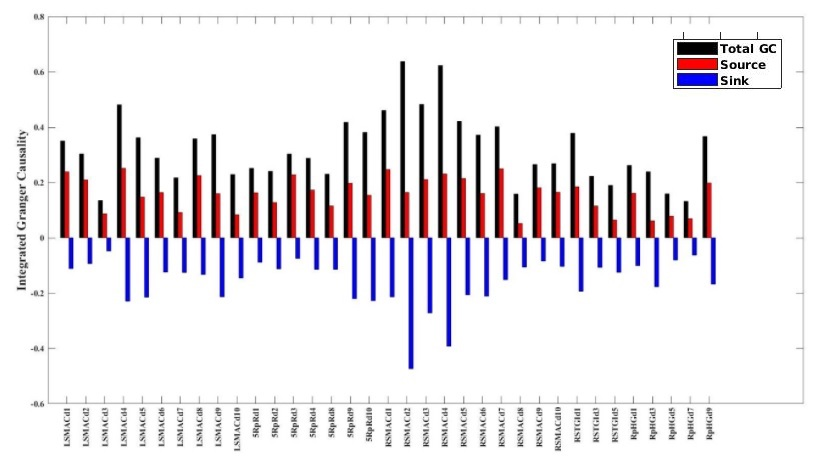
\includegraphics[height =3.5in]{Plots/GC_iEEG.jpg}
	}
	\caption{The total GC, source, sink activity as calculated from iEEG time series. RSMAcd3 and RSMAcd4 are two electrode contacts identified as EZ focus by neurologists. These two contacts are ranked among the highest for GC total and sink activity
	\label{fig:GC_EEG}
}
\end{figure*}

\begin{figure*}
\centerline{
	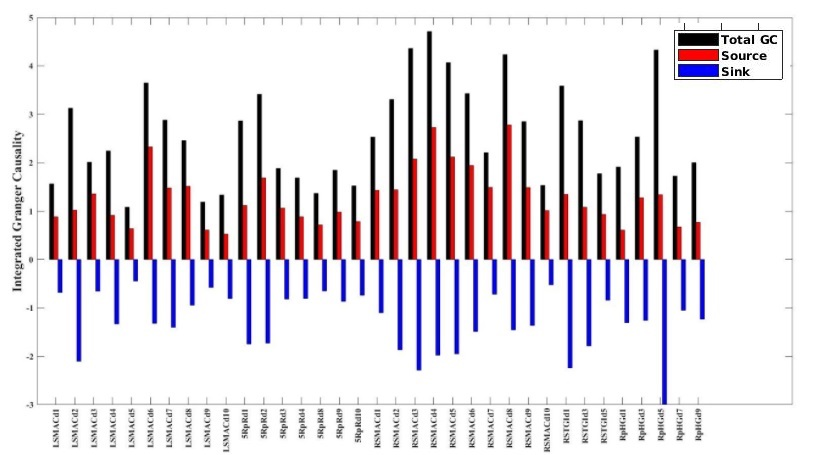
\includegraphics[height =3.5in]{Plots/GC_BOLD.jpg}
	}
	\caption{ Total Granger causality, source, sink activity as obtained from BOLD time series. RSMAcd3 and RSMAcd4 have comparatively higher Total GC and sink activity
	\label{fig:GC_BOLD}
}
\end{figure*}


\subsection{Graph theory}
Figure \ref{fig:betweenness_fmri_eeg}[a-b] shows the betweenness measure computed for iEEG and fMRI networks. The SO electrodes and the corresponding voxels RSMAcd is ranked top among 35 selected electrodes. The edges in the figure represents the strongest connection which was observed between RSMAcd and LSMAcd electrodes, located in opposite hemisphere. The next stronger connection of SO is with the hippocampus in both the networks, which is also considered as the generator of temporal epilespy \citep{avoli2007epileptic}. The connection is stronger in fMRI network compared to the iEEG network.


\begin{figure}%
    \centering
    a) {{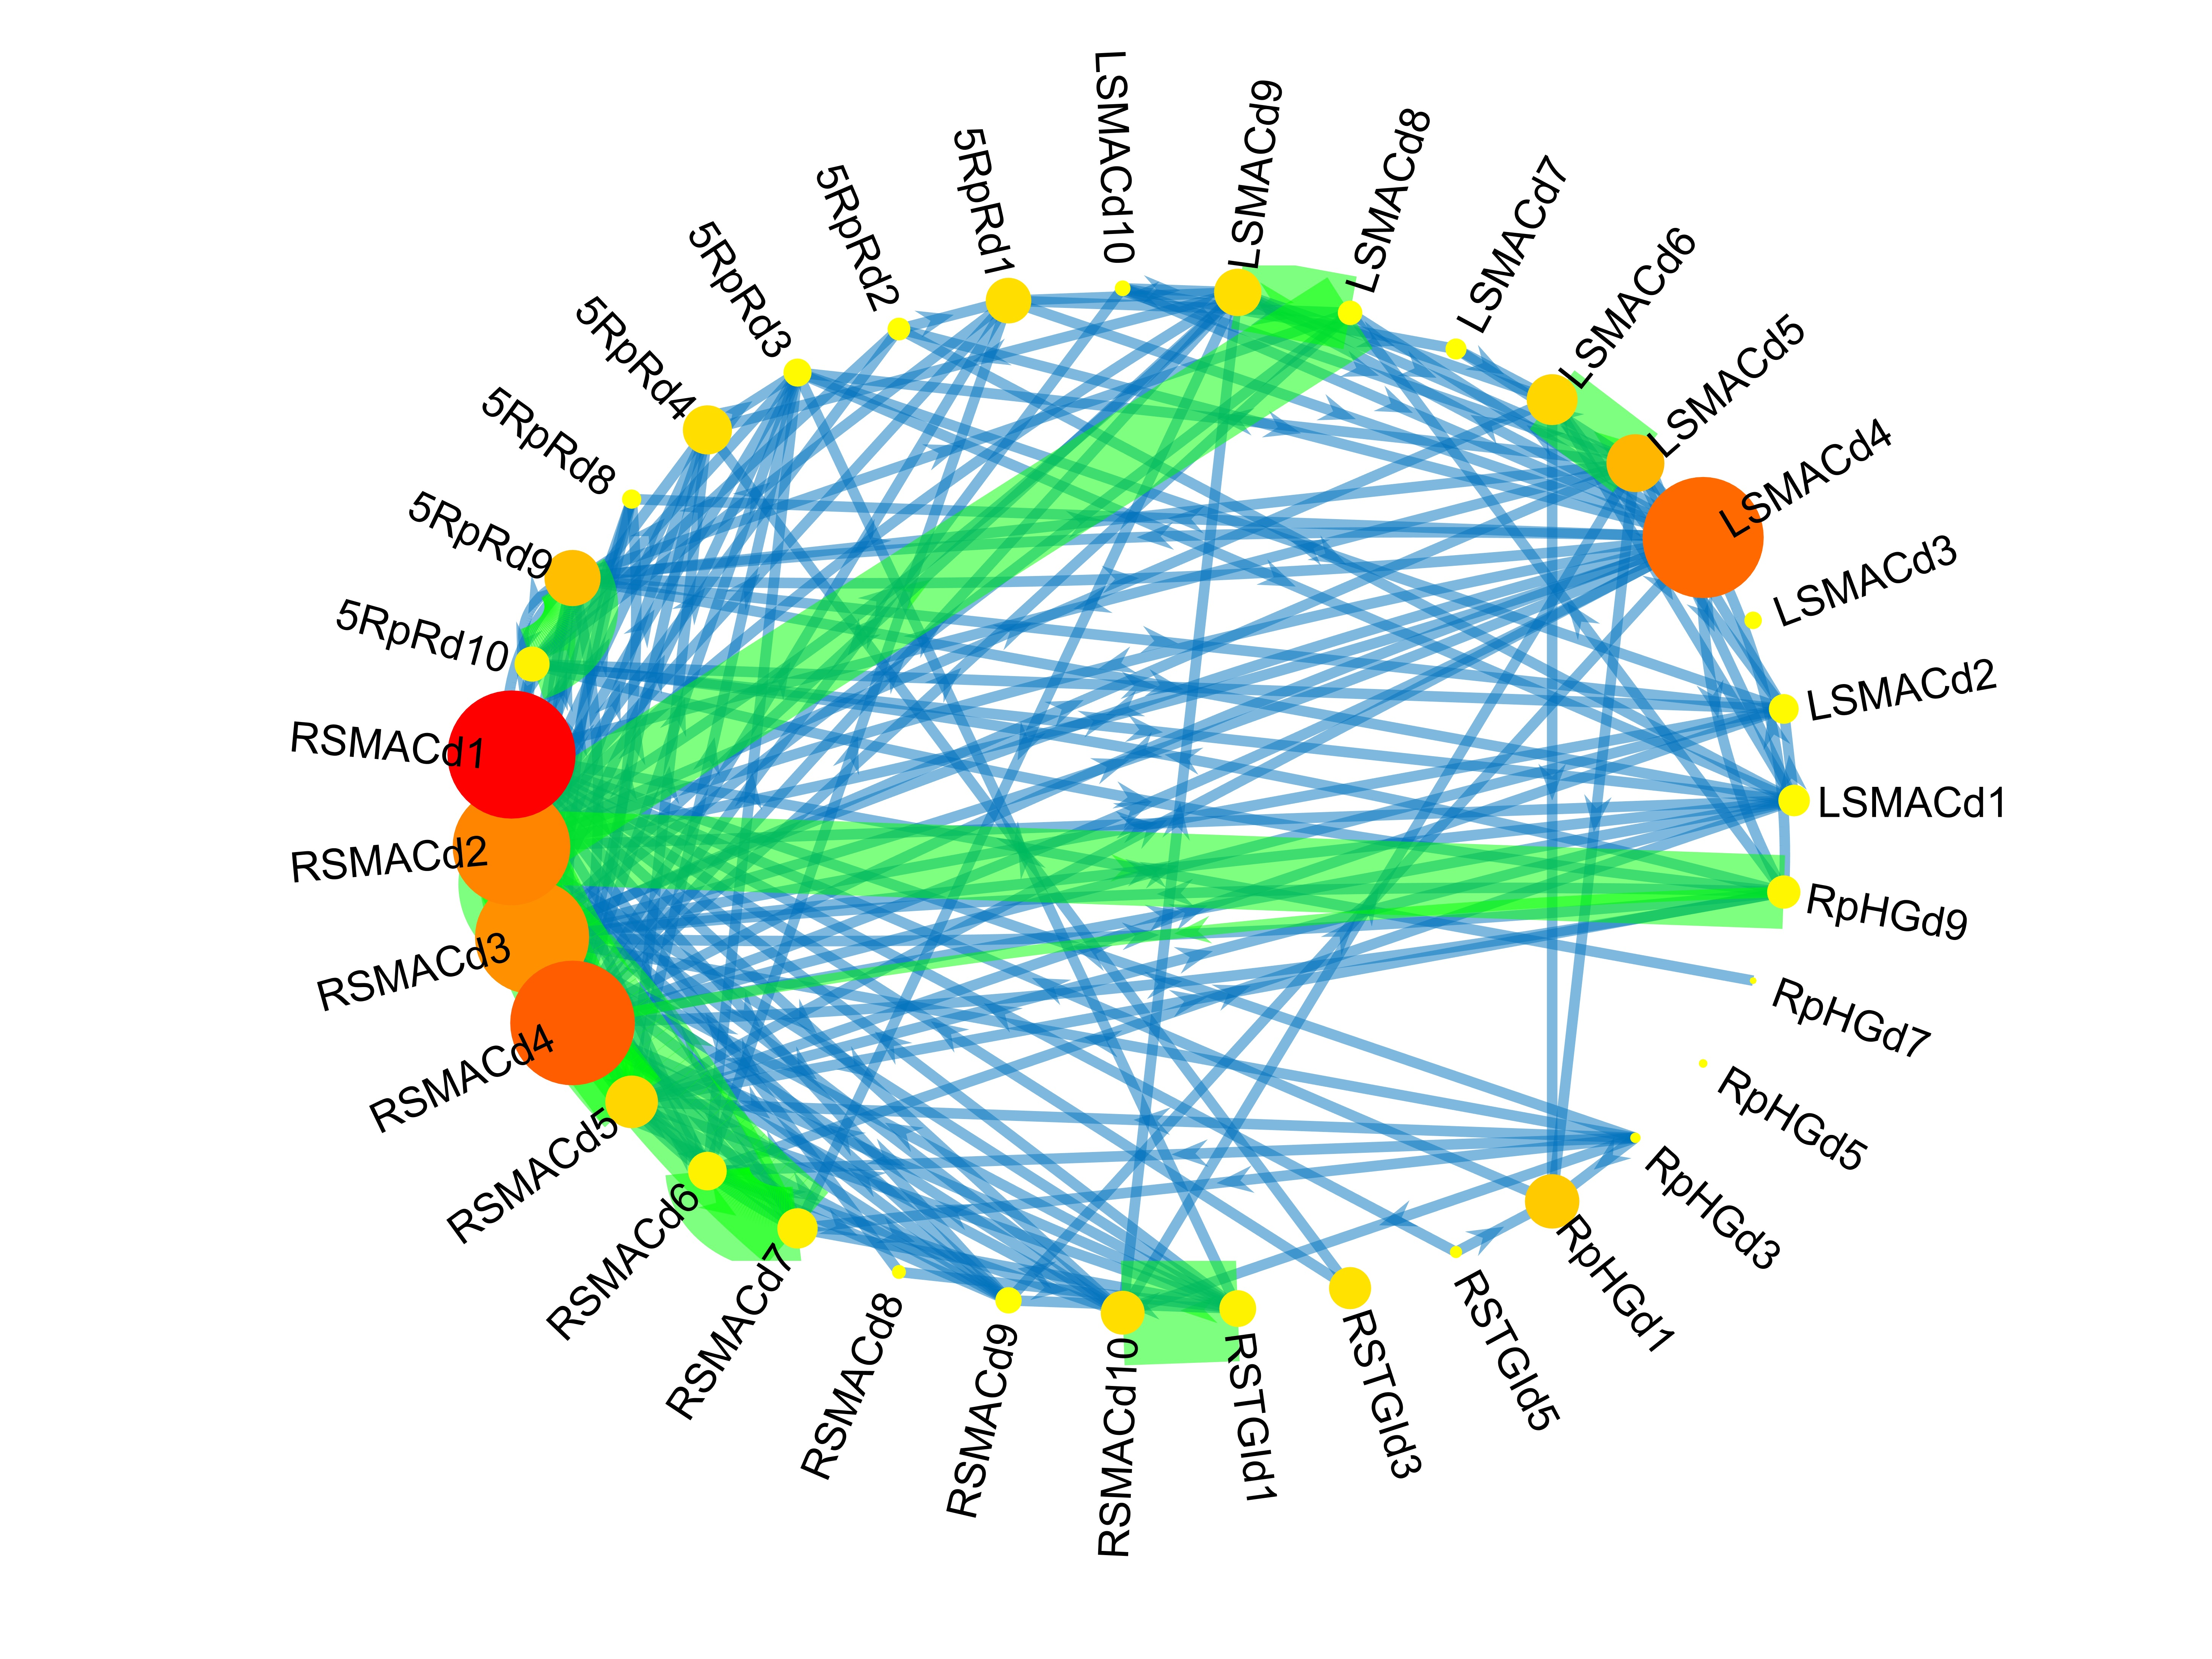
\includegraphics[width=13cm]{Plots/Patient_C_betweenness_ieeg.jpg} }}%
    
    b) {{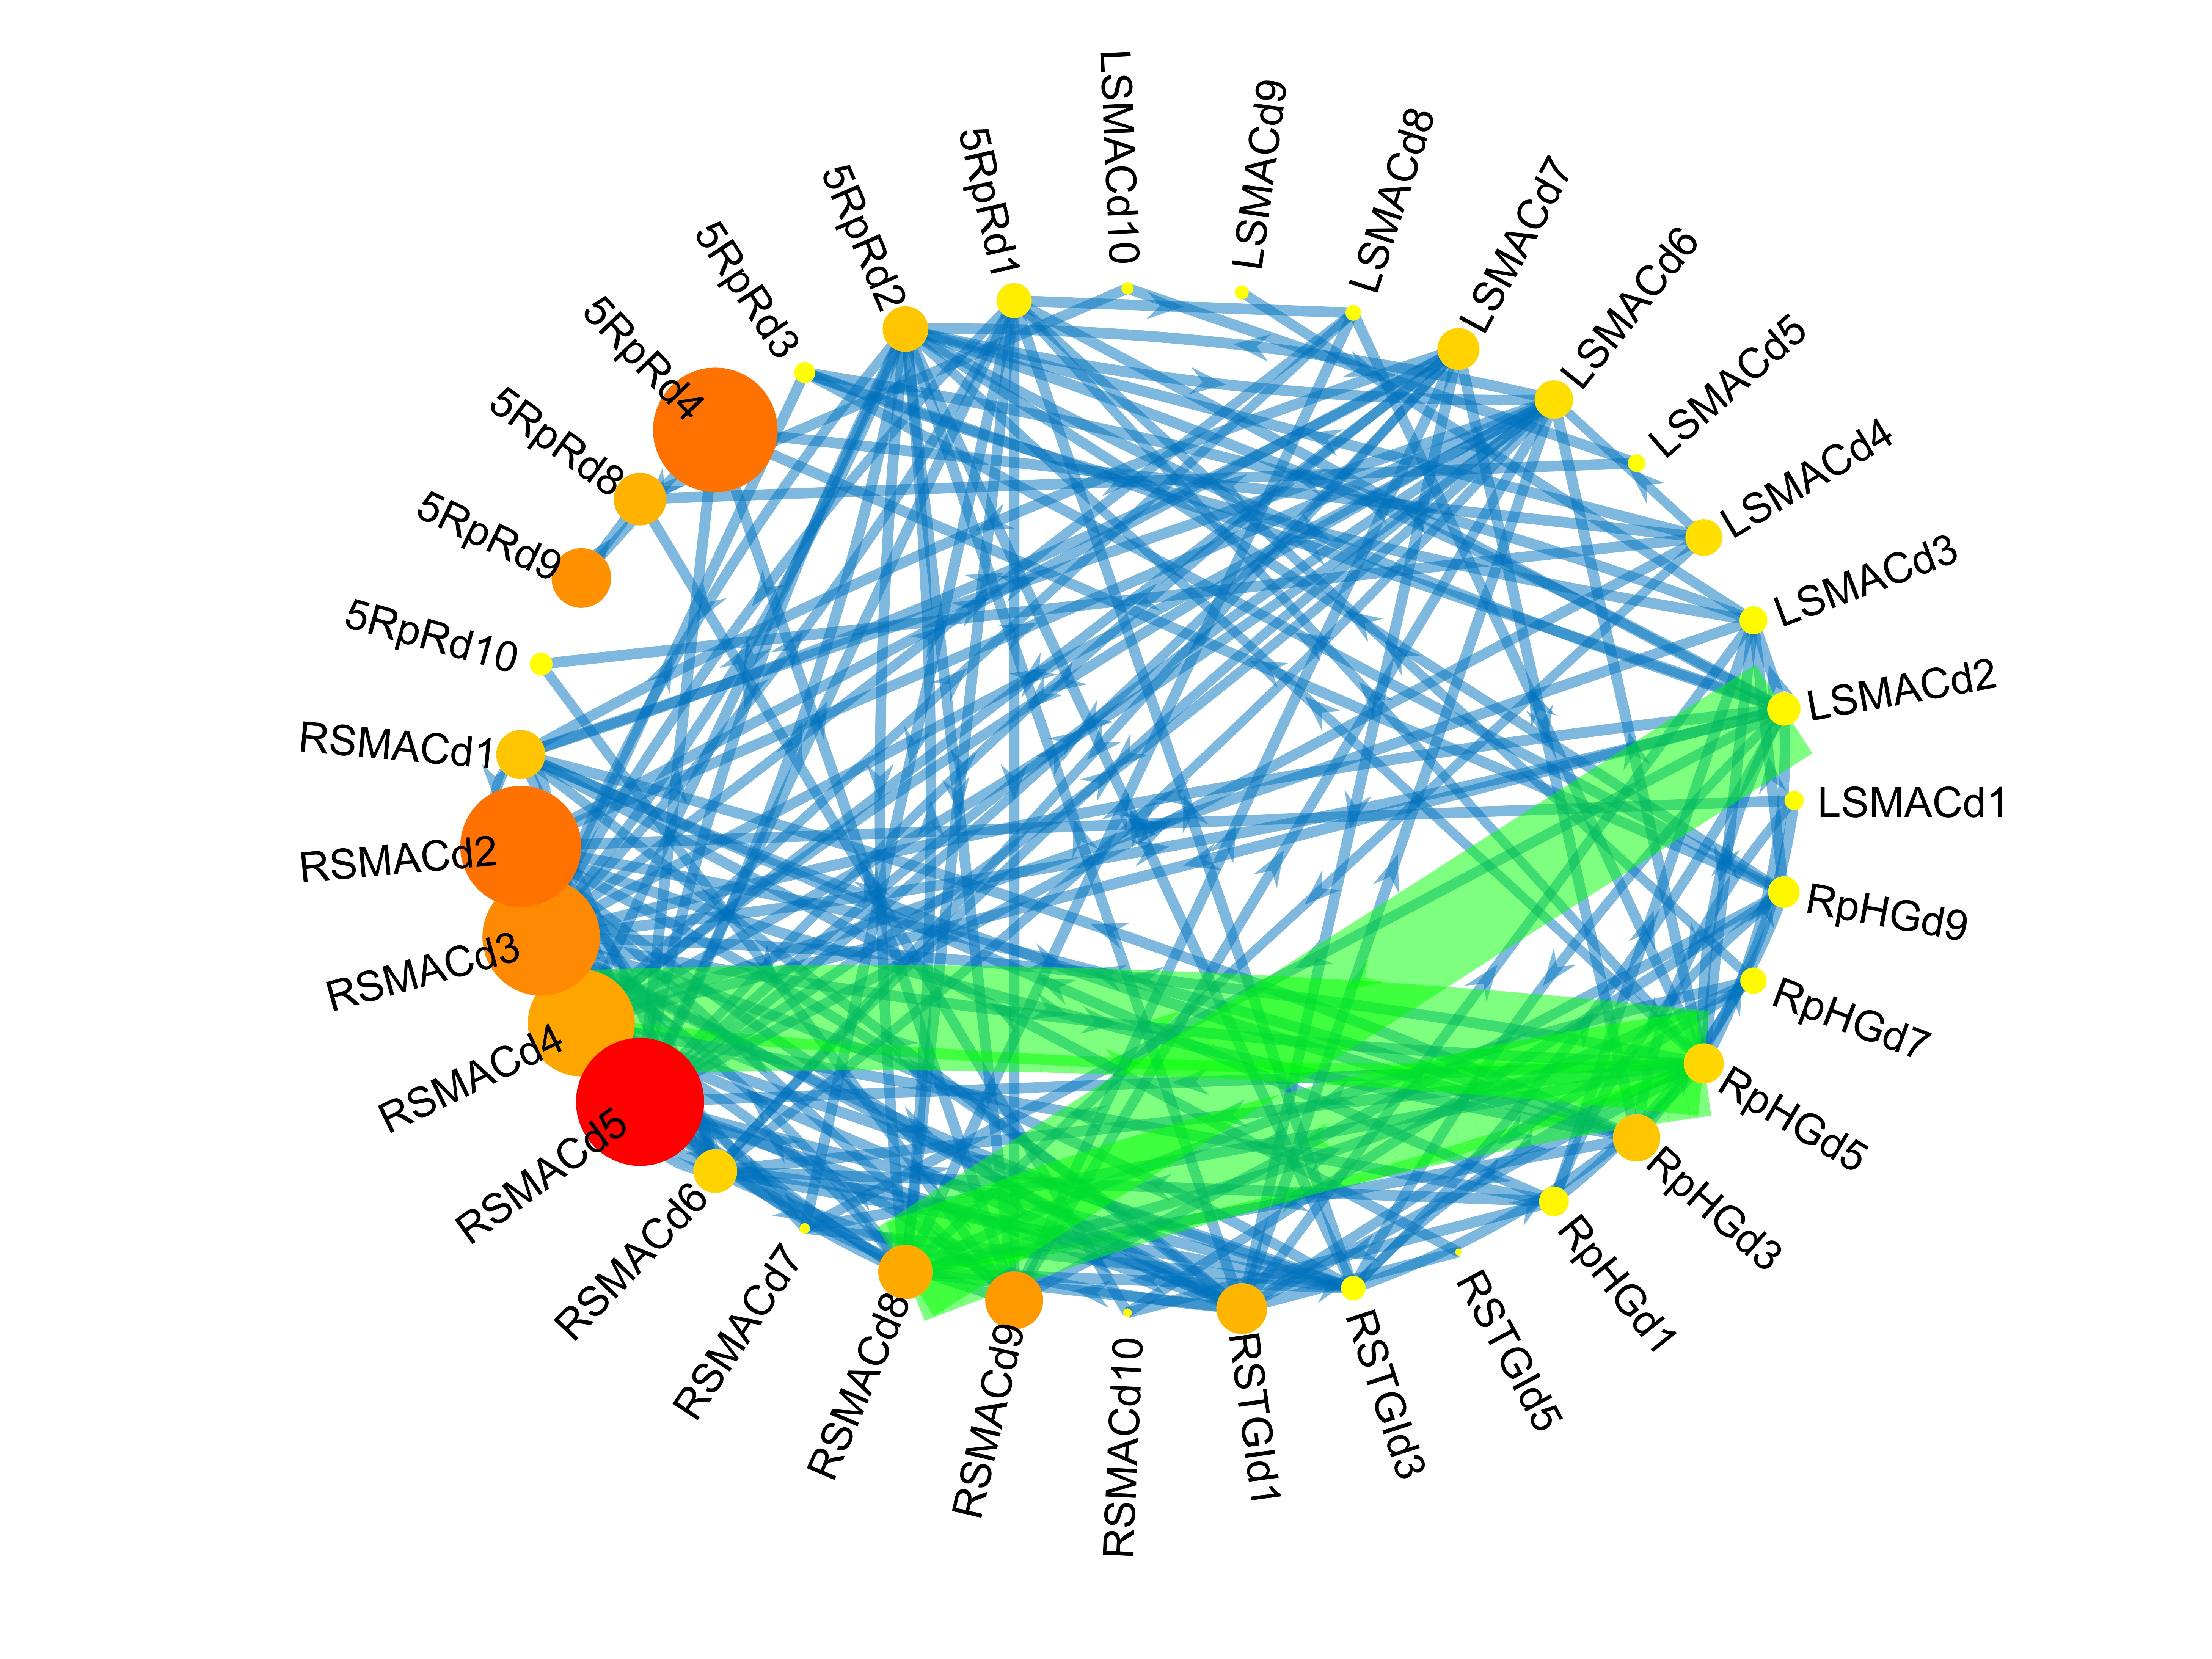
\includegraphics[width=13cm]{Plots/Patient_C_betweenness_fmri.jpg} }}%
    \caption{Betweenness measure computed from time domain Granger causality as adjacency matrix for a) iEEG, and b) fMRI. Red represents the node with the highest measure value and green represents the strongest edge or the connectivity strength. Strongest connection is observed between RSMAcd and LSMAcd electrodes.}%
    \label{fig:betweenness_fmri_eeg}%
\end{figure}


\begin{table}[]
\renewcommand{\arraystretch}{1.2} % Default value: 1
\setlength{\tabcolsep}{2pt} % Default value: 6pt
\centering
\begin{tabular}{|l|c|c|c|c|c|c|}
\hline
\multirow{2}{*}{\textbf{Measures}} & \multicolumn{2}{c|}{\textbf{4x4x4$mm^3$}}                                     & \multicolumn{2}{c|}{\textbf{6x6x6$mm^3$}}                                     & \multicolumn{2}{c|}{\textbf{8x8x8$mm^3$}}                                     \\ \cline{2-7}
                                   & \multicolumn{1}{l|}{\textbf{RSMAcd3}} & \multicolumn{1}{l|}{\textbf{RSMAcd4}} & \multicolumn{1}{l|}{\textbf{RSMAcd3}} & \multicolumn{1}{l|}{\textbf{RSMAcd4}} & \multicolumn{1}{l|}{\textbf{RSMAcd3}} & \multicolumn{1}{l|}{\textbf{RSMAcd4}} \\ \hline
Total GC                           & 17\%                                  & 27\%                                  & -                                     & \textbf{1\%}                          & \textbf{3\%}                          & \textbf{1\%}                          \\ \hline
Betweenness                        & -                                     & -                                     & -                                  & 17\%                                  & \textbf{5\%}                          & \textbf{6\%}                          \\ \hline
Degree                             & -                                     & -                                     & -                                     & \textbf{0.2\%}                        & \textbf{13\%}                         & \textbf{1\%}                          \\ \hline
Incloseness                        & -                                     & -                                     & -                                     & \textbf{1\%}                          & \textbf{4\%}                          & \textbf{3\%}                          \\ \hline
ClusteringCoef                    & -                                     & -                                     & -                                     & 26\%                                  & \textbf{4\%}                          & 17\%                                  \\ \hline
\end{tabular}
	\caption{The voxel wise analysis of gray matter on epileptic patients. SO electrodes RSMAcd3 and RSMAcd4 are ranked as percentage for four graph measures. N is the total number of voxels for each dimension. `-' represents non-significant results. Both SO electrodes lie within top 5\% for 8*8*8 $mm^3$ voxel dimension}
	\label{table:voxelwise_summary}
\end{table}

\subsection{Voxelwise analysis}
Previous computation was based upon the ROI extraction using spherical mask around the MNI coordinates. Some areas or voxels can be missed between two electrode contacts, which could potentially be the true seizure onzet zone. These regions can remain undetected using neuroimaging techniques or iEEG. To consider such regions, we varied the voxel dimensions (4x4x4 $mm^3$, 6x6x6 $mm^3$ and 8x8x8 $mm^3$) and computed the pairwise Granger causality between every other voxels in the gray matter.

\subsubsection{Rank of SO voxels}
The rankings of SO voxels among the total number of source voxels are shown in Table \ref{table:voxelwise_summary}. As we increase the voxel dimensions, total number of voxels in each voxel dimension decreases (15,462 voxels with $4*4*4mm^3$, 4,552 in 6*6*6 $mm^3$ and 1,959 in 8*8*8 $mm^3$). We ranked our result for each voxel in descending order of their magnitude for all measures. The percentage value is computed as the percent of rank of the SO electrode to the total number of voxels. As summarized in the table, the SO electrode RSMAcd4 is ranked within the top 1\% for 6x6x6 $mm^3$ voxel dimension for Total GC, Degree and Incloseness measures. Both the SO electrodes - RSMAcd3 and RSMAcd4 are among top 5\% in almost all measures for 8*8*8 $mm^3$ voxel dimension. '-' denotes that the result is not significant. The analysis for 10*10*10 $mm^3$ voxel dimension was not significant and it is not included in the table.


\begin{table}[]
\renewcommand{\arraystretch}{1.2} % Default value: 1
\setlength{\tabcolsep}{8pt} % Default value: 6pt
\centering
\begin{tabular}{|l|r|r|r|r|r|}
\hline
\multicolumn{1}{|c|}{\textbf{Measures\textbackslash MNI}} & \multicolumn{1}{c|}{\textbf{(2, -2, 40)}} & \multicolumn{1}{c|}{\textbf{(6, -6, 32)}} & \multicolumn{1}{c|}{\textbf{(6, 6, 40)}} & \multicolumn{1}{c|}{\textbf{(6, 6, 44)}} & \multicolumn{1}{c|}{\textbf{(10, 6, 44)}} \\ \hline
\textbf{Total GC}                                                & 79                                        & 173                                       & 88                                       & 506                                      & 244                                       \\ \hline
\textbf{Betweenness}                                             & 118                                       & 89                                        & 8                                        & 269                                      & 234                                       \\ \hline
\textbf{Degree}                                                  & 253                                       & 270                                       & 407                                      & 351                                      & 909                                       \\ \hline
\textbf{Incloseness}                                             & 88                                        & 392                                       & 154                                      & 178                                      & 709                                       \\ \hline
\textbf{Top R}                                                   & 79                                        & 89                                        & 8                                        & 178                                      & 234                                       \\ \hline
\textbf{Top ranked \%}                                           & 0.5\%                                     & 0.6\%                                     & 0.1\%                                    & 1.2\%                                    & 1.5\%                                     \\ \hline
% \textbf{Avg rank}                                                & 135                                       & 231                                       & 164                                      & 326                                      & 524                                       \\ \hline
% \textbf{Avg rank \%}                                            & 0.9\%                                     & 1.5\%                                     & 1.1\%                                    & 2.1\%                                    & 3.4\%                                     \\ \hline
\end{tabular}
	\caption{Rank of voxels located in the boundary of  8*8*8 $mm^3$ voxel in the site of SO electrodes}
	\label{table:rank_of_voxels_nearby_soe}
\end{table}


\subsubsection{Neighborhood around SO voxels}
The SO electrodes were ranked at the top for voxel dimension 8*8*8 $mm^3$ but not for 4*4*4 $mm^3$. This could be because the targeted voxel existed beyond the 4 mm voxel dimension but inside 8 mm. For the finer details, we focused on the spherical volume of radius 8mm around the center of SO electrodes as determined above and consider all 4x4x4 voxels within this boundary, and checked their rankings in the 4mm dimension, consisting of 15,562 voxels.

Table \ref{table:rank_of_voxels_nearby_soe} shows the ranks of 5 voxels that were constantly ranked highest for all 4 measures out of the 15,562 voxels. The measure for which the rank is topmost (i.e. lowest number in table) is selected as the top ranked voxel and its percentage is shown in the top ranked percentage row. The voxel with MNI coordinate (6, 6, 40) was ranked $8^{th}$ out of 15,462 voxels for the betweenness measure. This voxel is also ranked within top 5 percentage for all other measures. Similarly the nearby voxel (2, -2, 40) was ranked among top 5 percentage for total GC and betweenness among these 5 voxels. However, it is possible that the voxel (6, 6, 40) represents the prime voxel for seizure onset, being located very close to the identified SO electrode RSMAcd4, and ranked at the 0.05 percentile for the entire brain using the betweenness measure. 


\begin{figure*}
\centerline{
	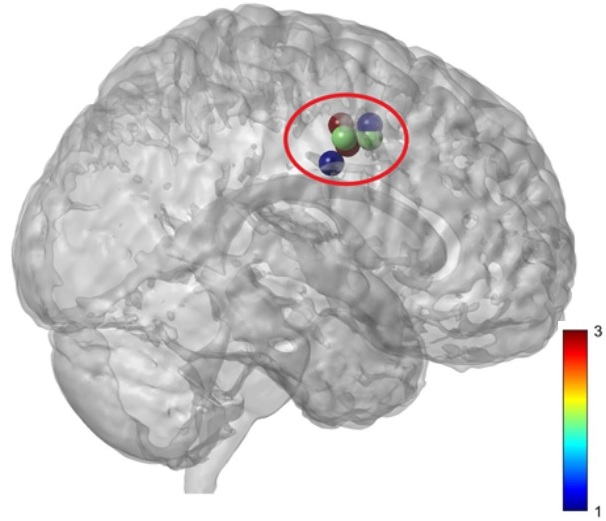
\includegraphics[height =3in]{Plots/top_voxels.jpg}
	}
	\caption{ Top voxels according to total causal flow and three graph measures located within the boundary of 8*8*8 $mm^3$ voxels dimension. Two red dots are SO voxels - RSMAcd3 and RSMAcd4 with voxel dimension 4*4*4 dimension. (2,-2,40) and (6, 6, 40) are represented as green dots. Blue dots are the other three voxels.
	\label{fig:top_voxels}
}
\end{figure*}

\begin{figure*}
\centerline{
	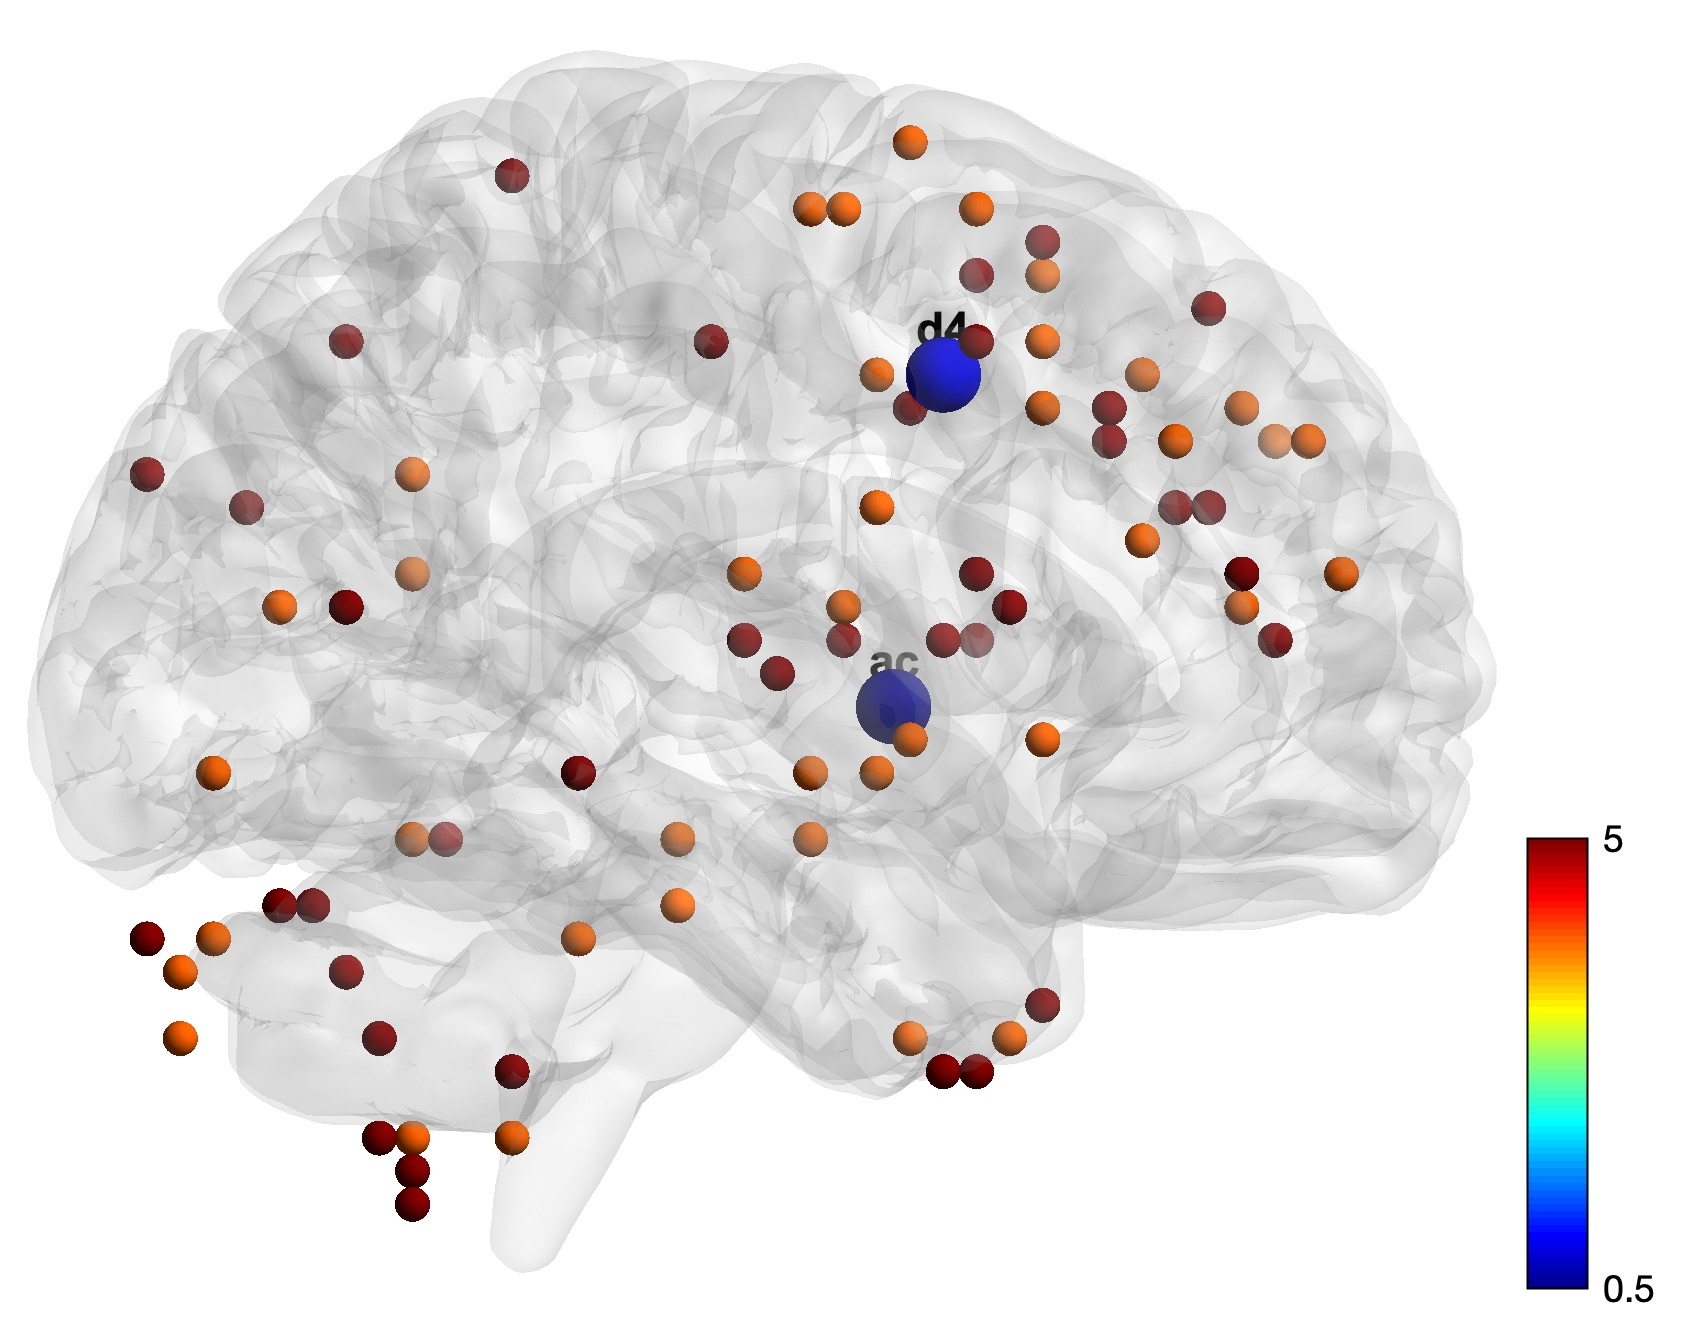
\includegraphics[height =3in]{Plots/Patient_C_eegfmri_voxel_cluster.jpg}
	}
	\caption{ The top 80 connections from the $8^{th}$ top ranked (6, 6, 40) voxel of over 12,000. The outflow clusters are observed in frontal lobes, cerebellum, basal ganglia and thalamus.
	\label{fig:top_voxel_cluster}
}
\end{figure*}

%This voxel lies at d4 and anterior commisure (ac) is the centre or the reference point of the brain.

Figure \ref{fig:top_voxels} illustrates the top voxels of 4*4*4 $mm^3$ voxel dimension located within the boundary of 8*8*8 $mm^3$ voxel dimension right in the location of SO electrodes. 

%We observed that different voxels were ranked highest for different measures instead of single voxels as the maximum of all measures. The averages of these voxels might have been the reason behind the maximum value and consistently significant result for 8*8*8 $mm^3$ voxels dimension. We were able to find the seizure onset voxel in voxel dimensions as small as 4*4*4 voxel $mm^3$.

Figure \ref{fig:top_voxel_cluster} shows the strongest connections from the top ranking voxel (8 out of 15,000) to the whole brain. The connections of this voxel cluster around frontal lobes, cerebellum, basal ganglia and thalamus. These areas have a major role in cognition, decision making and motor control. This result demonstrates the connection between seizure origin and other areas. The impairment of these clustered areas could be associated with the seizure symptoms.


\section{Discussion}
\label{sec:discussion}
In this study, we used quantitative techniques based on Granger causality and graph theory to study the correlation between iEEG and BOLD signals from resting state fMRI. Our results showed that the iEEG electrode contacts with the strongest infra-slow EEG signal correlated with the spontaneous BOLD fluctuations in corresponding location. The voxels within a small radius of the seeded location were constantly significant for total causal flow and directed centrality measures like betweenness, degree and incloseness. Individual voxel analysis within this radius showed a highly significant clustering based on various measures when compared to other voxels throughout the entire brain.

We compared the causal relationship of the total causal flow and sink activity between the infra-slow interictal iEEG time-series and the corresponding fMRI BOLD signal. However, causal relationship was not overlapped for the same range of infra-slow frequency range. The infraslow frequency range considered for BOLD signal was longer than that for iEEG. Based on our multiple experiments on different frequency ranges, we found that the frequency range 0.01-0.2 Hz in iEEG and 0.08-0.8 Hz in fMRI have the highest coupling between each other and the SO electrodes. This result could be patient specific, and multiple patients have to be studied to find the average overlap range of infraslow frequency between iEEG and fMRI.

The voxelwise analysis of whole brain showed that the voxels in the proximity of seeded locations resulted in the top rank for the computed quantitative measures.The electrical activity recorded in SO iEEG electrodes might have been influenced by these cluster of voxels as \citep{menon1996spatio} illustrated that the distribution of coherence values differed from background level at interisite distances of 1 and 1.4 cm for iEEG electrodes. Prolonged seizure freedom by a small laser resection strongly supports the iEEG indications that the presumed focus did indeed include the true seizure onset zone. 

%The reason for the patient to be seizure free could be the removal of this area along with the targeted brain area by laser surgery. The other reason for this significant cluster could be due to the mismatch between seizure onset zone (SOZ) and the corresponding seeding in fMRI. The SOZ, identified in fMRI scan, could have been shifted by a few millimeters due to swelling or the invasion by implanted electrodes.

We acknowledge the challenges in comparing EEG and BOLD signals. Few previous studies have used functional connectivity measures in the two signals,  similar to our approach. Instead, we follow the same methods of functional connectivity method - Granger causality and graph measures, for both iEEG and BOLD signals, similar to our analysis of high-frequency infra-slow iEEG time-series for different phases of epilepsy. 

The iEEG and BOLD signals not being recorded simultaneously is another challenge. As discussed by Aghakhani and team, the BOLD signal from true seizure onset areas could be distorted in simultaneous iEEG-fMRI due to implanted electrodes \citep{aghakhani2015co}. The time of acquisition of fMRI and iEEG signals differed by several months in our study. Neuroimaging and iEEG studies have confirmed that significant progression of the epilep- togenic process might progress over several years in epilepsy \citep{walker2002disease}. However, the locations of the SOZ appear nearly identical in our dataset.

The other challenges include the computation time for connectivity measures with a large number of voxels. We limited our analysis to $4_{mm}^3$ voxel dimensions as the computation boundary of the cluster computer in our lab. The number of voxels would increase to hundred of thousands as we increase the resolution to $2_{mm}^3$ voxels, the highest resolution of fMRI with present day scanners. The correlations between the neighboring voxels can be profound at this level and the result could be compromised. We also limited our study of causality to pairwise parametric Granger causality, instead of a non-parametric method for the same reason. However, we determined model order by comparing spectral power between parametric and non-parametric methods for the validation of autoregressive model fitting of the data. These two issues related to computation time could be resolved in the future with more efficient algorithms and more powerful computing resources. 

Despite these challenges and limitations, we are able to demonstrate that using the intracranial ictal EEG recording as a seed, the infraslow EEG activity is highly correlated with the corresponding voxels of the resting state functional MRI (rsfMRI) recorded months before. As such, intracranial EEG has the potential to be used as a seed in the rsfMRI to characterize the epilepsy focus and connections of the epilepsy network throughout the entire brain at milimeters resolution. 

Nonetheless, the fine detail mapping of the epilepsy network presented in this study requires further extensive testing and analysis to determine the optimal methods for characterizing and displaying the results. As with other applications of RSfMRI, causal analysis, and graph theory, a great variety of techniques are feasible. Obvious questions of importance include the percentage of potential epilepsy surgery patients in whom the focus can be this precisely defined, including those with visible lesions or possible tandem foci; and whether combining them with cluster analysis may allow the application of these techniques to the interictal resting state fMRI alone.
%!TEX root = ../main.tex

\chapter{Summary and Future Directions}
\label{chapter-summary}

%\section{Summary}
In this dissertation, we have provided the first comprehensive quantitative analysis of infraslow iEEG recording from human subjects using intracranial electrodes. We have performed for the first time a quantitative analysis of the information contents of different frequency components in the infraslow iEEG signal. We showed that the strongest infraslow iEEG signal correlates highly with the location of the visible seizure focus, and also with that of the strongest high frequency EEG signal as well, in both the preictal and interictal phases of the epilepsy cycle. In different patients and phases this signal may be more prominent in either total or negative causal flow.

We then demonstrated that the iEEG electrode contacts showing the strongest infraslow iEEG signal correlated with voxels with the strongest resting state fMRI (rsfMRI) signal at the corresponding locations, using similar methods of frequency analysis; and that those those voxels form a highly significant grouping when compared to others throughout the entire brain. Finally, having seeded the epilepsy focus into the rffMRI, we have begun mapping the connections of the epilepsy network throughout the entire brain in unprecedented fine detail.
These exciting results make a crucial contribution to our understanding of epileptic seizure propagation and open up new possibilities for localizing seizure onset zones non-invasively.

%\section{Future Directions}

% \begin{itemize}

% \item Expand the study on more retrospective and prospective patients to standardize our methodology. 

% \item Extensive testing and analysis to determine the optimal methods for characterizing and displaying the results

% \item Explore other quantitative techniques besides Granger causality and graph measures

% \end{itemize}

%Notes to edit: Optimal fine detail mapping of the epilepsy network using the techniques we have pioneered requires further extensive testing and analysis to determine the optimal methods for characterizing and displaying the results. As with other applications of RSfMRI, causal analysis, and graph theory, a great variety of techniques are feasible. Obvious questions of importance include the percentage of potential epilepsy surgery patients in whom the focus can be this precisely defined, including those with visible lesions or possible tandem foci; and whether, having identified optimal methods, combining them with cluster analysis may allow the application of these techniques to the IRSfMRI alone.

Having used infraslow EEG analysis to seed the epilepsy focus into the rsfMRI, we will continue mapping in fine detail the connections of the epilepsy network throughout the entire brain, and extend our techniques to additional patients. Through testing of multiple causal and graph theory parameters, we will identify those that best allow characterization of the epilepsy focus voxels as a discrete cluster. Then, using additional methods of cluster analysis, we hope that our techniques may allow the precise identification of the focus and network without seeding from the iEEG, but directly from the rsfMRI.

%%%%%%%%%%%%%%%%%%%% The backmatter goes in this file %%%%%%%%%%%%%%%%%%%%%

% The bibliography starts here.

\bibliographystyle{apj}             % Please learn to use the
                                    % formatting of Latex's Bibtex. It
                                    % will make your life easier.

\bibliography{bibliography}
%\bibliography{apj-jour,dissref}       % "paper.bib" contains all my
                                    % references. "apj-jour.bib"
                                    % contains abbreviations of
                                    % journals.


\clearpage
% If you have only one appendix chapter, use the command
% \begin{appendix}...\end{appendix} instead.
% This takes care of the requirement (of the Graduate Office) for one
% appendix chapter to be labeled as 'Appendix', not 'Appendix A'.

\beforechapterheadname{APPENDIX}         % Optional text to put in front of
                                   % the chapter number.
\afterchapterheadname{}          % Optional text to put after the

\addcontentsline{toc}{chapter}{APPENDIX}

%\begin{appendix}
%  \input{appendixI}                     % Your appendices go here.
%  %%
%% This is file `appendix.sty',
%% generated with the docstrip utility.
%%
%% The original source files were:
%%
%% appendix.dtx  (with options: `usc')
%%
%% -----------------------------------------------------------------
%%   Author: Peter Wilson (CUA) now at peter.r.wilson@boeing.com until June 2004
%%                              (or at: pandgwilson at earthlink dot net)
%%   Copyright 1998 --- 2004 Peter R. Wilson
%%
%%   This work may be distributed and/or modified under the
%%   conditions of the LaTeX Project Public License, either
%%   version 1.3 of this license or (at your option) any
%%   later version.
%%   The latest version of the license is in
%%      http://www.latex-project.org/lppl.txt
%%   and version 1.3 or later is part of all distributions of
%%   LaTeX version 2003/06/01 or later.
%%
%%   This work has the LPPL maintenance status "author-maintained".
%%
%%   This work consists of the files listed in the README file.
%% -----------------------------------------------------------------
%%
\NeedsTeXFormat{LaTeX2e}
\ProvidesPackage{appendix}[2002/08/06 v1.2 extra appendix facilities]

\newif\if@chapter@pp\@chapter@ppfalse
\newif\if@knownclass@pp\@knownclass@ppfalse
\@ifundefined{chapter}{%
  \@ifundefined{section}{}{\@knownclass@pptrue}}{%
  \@chapter@pptrue\@knownclass@pptrue}
\providecommand{\phantomsection}{}
\newcounter{@pps}
  \renewcommand{\the@pps}{\alph{@pps}}
\newif\if@pphyper
  \@pphyperfalse
\AtBeginDocument{%
  \@ifpackageloaded{hyperref}{\@pphypertrue}{}}

\newif\if@dotoc@pp\@dotoc@ppfalse
\newif\if@dotitle@pp\@dotitle@ppfalse
\newif\if@dotitletoc@pp\@dotitletoc@ppfalse
\newif\if@dohead@pp\@dohead@ppfalse
\newif\if@dopage@pp\@dopage@ppfalse
\DeclareOption{toc}{\@dotoc@pptrue}
\DeclareOption{title}{\@dotitle@pptrue}
\DeclareOption{titletoc}{\@dotitletoc@pptrue}
\DeclareOption{header}{\@dohead@pptrue}
\DeclareOption{page}{\@dopage@pptrue}
\ProcessOptions\relax
\newcommand{\@ppendinput}{}
\if@knownclass@pp\else
  \PackageWarningNoLine{appendix}%
    {There is no \protect\chapter\space or \protect\section\space command.\MessageBreak
     The appendix package will not be used}
  \renewcommand{\@ppendinput}{\endinput}
\fi
\@ppendinput

\newcommand{\appendixtocon}{\@dotoc@pptrue}
\newcommand{\appendixtocoff}{\@dotoc@ppfalse}
\newcommand{\appendixpageon}{\@dopage@pptrue}
\newcommand{\appendixpageoff}{\@dopage@ppfalse}
\newcommand{\appendixtitleon}{\@dotitle@pptrue}
\newcommand{\appendixtitleoff}{\@dotitle@ppfalse}
\newcommand{\appendixtitletocon}{\@dotitletoc@pptrue}
\newcommand{\appendixtitletocoff}{\@dotitletoc@ppfalse}
\newcommand{\appendixheaderon}{\@dohead@pptrue}
\newcommand{\appendixheaderoff}{\@dohead@ppfalse}
\newcounter{@ppsavesec}
\newcounter{@ppsaveapp}
\setcounter{@ppsaveapp}{0}
\newcommand{\@ppsavesec}{%
  \if@chapter@pp \setcounter{@ppsavesec}{\value{chapter}} \else
                 \setcounter{@ppsavesec}{\value{section}} \fi}
\newcommand{\@pprestoresec}{%
  \if@chapter@pp \setcounter{chapter}{\value{@ppsavesec}} \else
                 \setcounter{section}{\value{@ppsavesec}} \fi}
\newcommand{\@ppsaveapp}{%
  \if@chapter@pp \setcounter{@ppsaveapp}{\value{chapter}} \else
                 \setcounter{@ppsaveapp}{\value{section}} \fi}
\newcommand{\restoreapp}{%
  \if@chapter@pp \setcounter{chapter}{\value{@ppsaveapp}} \else
                 \setcounter{section}{\value{@ppsaveapp}} \fi}
\providecommand{\appendixname}{APPENDIX}
\newcommand{\appendixtocname}{APPENDICES}
\newcommand{\appendixpagename}{APPENDICES}
\newcommand{\appendixpage}{%
%  \if@chapter@pp \@chap@pppage \else \@sec@pppage \fi
  \if@chapter@pp \else \@sec@pppage \fi
}
\newcommand{\clear@ppage}{%
  \if@openright\cleardoublepage\else\clearpage\fi}

\newcommand{\@chap@pppage}{%
%  \clear@ppage
%  \thispagestyle{plain}%
  \if@twocolumn\onecolumn\@tempswatrue\else\@tempswafalse\fi
%  \null\vfil
%  \markboth{}{}%
  {\centering
%   \interlinepenalty \@M
   \normalfont
   \normalsize \bfseries \appendixpagename\par}%
  \if@dotoc@pp
    \addappheadtotoc
  \fi
  \vfil%\newpage
  \if@twoside
    \if@openright
%      \null
%      \thispagestyle{empty}%
      %\newpage
    \fi
  \fi
  \if@tempswa
    \twocolumn
  \fi
}

\newcommand{\@sec@pppage}{%
  \par
  \addvspace{4ex}%
  \@afterindentfalse
  {\parindent \z@ \raggedright
   \interlinepenalty \@M
   \normalfont
   \normalsize \bfseries \appendixpagename%
   \markboth{}{}\par}%
  \if@dotoc@pp
    \addappheadtotoc
  \fi
  \nobreak
  \vskip 3ex
  \@afterheading
}

\newif\if@pptocpage
  \@pptocpagetrue
\newcommand{\noappendicestocpagenum}{\@pptocpagefalse}
\newcommand{\appendicestocpagenum}{\@pptocpagetrue}
\newcommand{\addappheadtotoc}{%
  \phantomsection
  \if@chapter@pp
    \if@pptocpage
      \addcontentsline{toc}{chapter}{\appendixtocname}%
    \else
      \if@pphyper
        \addtocontents{toc}%
          {\protect\contentsline{chapter}{\appendixtocname}{}{\@currentHref}}%
      \else
        \addtocontents{toc}%
          {\protect\contentsline{chapter}{\appendixtocname}{}}%
      \fi
    \fi
  \else
    \if@pptocpage
      \addcontentsline{toc}{section}{\appendixtocname}%
    \else
      \if@pphyper
        \addtocontents{toc}%
          {\protect\contentsline{section}{\appendixtocname}{}{\@currentHref}}%
      \else
        \addtocontents{toc}%
          {\protect\contentsline{section}{\appendixtocname}{}}%
      \fi
    \fi
  \fi
}

\providecommand{\theH@pps}{\alph{@pps}}

\newcommand{\@resets@pp}{\par
  \@ppsavesec
  \stepcounter{@pps}
  \setcounter{section}{0}%
  \if@chapter@pp
    \setcounter{chapter}{0}%
    \renewcommand\@chapapp{\appendixname}%
     \ifthenelse{\equal{\thechapter}{}}{\renewcommand\thesection{\@Alph\c@section}}{\renewcommand\thechapter{\@Alph\c@chapter}}
  \else
    \setcounter{subsection}{0}%
    \renewcommand\thesection{\@Alph\c@section}%
  \fi
  \if@pphyper
    \if@chapter@pp
      \renewcommand{\theHchapter}{\theH@pps.\Alph{chapter}}%
    \else
      \renewcommand{\theHsection}{\theH@pps.\Alph{section}}%
    \fi
    \def\Hy@chapapp{\appendixname}%
  \fi
  \restoreapp
}

\newenvironment{appendices}{%
  \@resets@pp
  \if@dotoc@pp
    \if@dopage@pp              % both page and toc
      \if@chapter@pp           % chapters
%        \clear@ppage
      \fi
      \appendixpage
    \else                      % toc only
       \if@chapter@pp          % chapters
%         \clear@ppage
       \fi
      \addappheadtotoc
    \fi
  \else
    \if@dopage@pp              % page only
      \appendixpage
    \fi
  \fi
  \if@chapter@pp
    \if@dotitletoc@pp \@redotocentry@pp{chapter} \fi
  \else
    \if@dotitletoc@pp \@redotocentry@pp{section} \fi
    \if@dohead@pp
      \def\sectionmark##1{%
        \if@twoside
          \markboth{\@formatsecmark@pp{##1}}{}
        \else
          \markright{\@formatsecmark@pp{##1}}{}
        \fi}
    \fi
    \if@dotitle@pp
      \def\sectionname{\appendixname}
      \def\@seccntformat##1{\@ifundefined{##1name}{}{\csname ##1name\endcsname\ }%
        \csname the##1\endcsname\quad}
    \fi
  \fi}{%
  \@ppsaveapp\@pprestoresec}

\newcommand{\setthesection}{\thechapter.\Alph{section}}
\newcommand{\setthesubsection}{\thesection.\Alph{subsection}}

\newcommand{\@resets@ppsub}{\par
  \stepcounter{@pps}
  \if@chapter@pp
    \setcounter{section}{0}
    \renewcommand{\thesection}{\setthesection}
  \else
    \setcounter{subsection}{0}
    \renewcommand{\thesubsection}{\setthesubsection}
  \fi
  \if@pphyper
    \if@chapter@pp
      \renewcommand{\theHsection}{\theH@pps.\setthesection}%
    \else
      \renewcommand{\theHsubsection}{\theH@pps.\setthesubsection}%
    \fi
    \def\Hy@chapapp{\appendixname}%
  \fi
}

\newenvironment{subappendices}{%
  \@resets@ppsub
  \if@chapter@pp
    \if@dotitletoc@pp \@redotocentry@pp{section} \fi
    \if@dotitle@pp
      \def\sectionname{\appendixname}
      \def\@seccntformat##1{\@ifundefined{##1name}{}{\csname ##1name\endcsname\ }%
        \csname the##1\endcsname\quad}
    \fi
  \else
    \if@dotitletoc@pp \@redotocentry@pp{subsection} \fi
    \if@dotitle@pp
      \def\subsectionname{\appendixname}
      \def\@seccntformat##1{\@ifundefined{##1name}{}{\csname ##1name\endcsname\ }%
        \csname the##1\endcsname\quad}
    \fi
  \fi}{}

\newcommand{\@formatsecmark@pp}[1]{%
  \MakeUppercase{\appendixname\space
    \ifnum \c@secnumdepth >\z@
      \thesection\quad
    \fi
    #1}}
\newcommand{\@redotocentry@pp}[1]{%
  \let\oldacl@pp=\addcontentsline
  \def\addcontentsline##1##2##3{%
    \def\@pptempa{##1}\def\@pptempb{toc}%
    \ifx\@pptempa\@pptempb
      \def\@pptempa{##2}\def\@pptempb{#1}%
      \ifx\@pptempa\@pptempb
\oldacl@pp{##1}{##2}{\appendixname\space ##3}%
      \else
        \oldacl@pp{##1}{##2}{##3}%
      \fi
    \else
      \oldacl@pp{##1}{##2}{##3}%
    \fi}
}

\endinput
%%
%% End of file `appendix.sty'.
                     %named "appendix.tex"
%\end{appendix}
               % See the backmatter.tex file

\appendix
\section*{Appendices}
\addcontentsline{toc}{section}{Appendices}
\renewcommand{\thesubsection}{\Alph{subsection}}

\chapter{Definitions - Granger causality and graph measures}
\label{chapter:appendix-definitions}

\section{Granger causality}
Given two simultaneously measured time series $X_{1}(t)$ and $X_{2}(t)$, we compute the covariance matrix ($\Sigma$), the transformation function ($H(f)$) by multivariate vector autoregressive modeling of the time series \citep{dhamala2008analyzing, dhamala2008estimating}, and the spectral density matrix ($S(f)$) from these time series, such that $S(f) = H(f) \sum H*(f)$. 

The noise covariance matrix ($\Sigma$) is computed from the residual errors of the prediction models, and the transfer function $H$ is obtained from the matrix inverse of the Fourier transforms of the coefficients in the prediction models. For non-stationary process, $S, H,$ and $\Sigma$ can be estimated using the wavelet transforms-based non-parametric estimation \citep{dhamala2008estimating}, so that these quantities become the function of both time and frequency domains.

The spectral GC from 2 to 1, $M_{2 \rightarrow 1}(f)$ can be obtained as

\[ M_{2\rightarrow1}(f) = -\ln \frac{S_{11}(f) - (\sum_{22}- \frac{\sum^2_{12}}{\sum_{11}} ) | H_{12}(f) |^2 }{S_{11}(f)}\] 

where, by interchanging 1 and 2, one can compute the spectral GC from 1 to 2, $M_{1 \rightarrow 2}(f)$.
The time-domain Granger causality can be obtained by integration over the entire frequency range.
The total interdependency measures of statistically inter-related two stationary
processes consists of sub-measures and can be expressed as;
\[ M_{1,2} = M_{1 \rightarrow 2} + M_{2 \rightarrow 1} + M_{1.2} \]
where $M_{2 \rightarrow 1}$ and $M_{1 \rightarrow 2}$ are one-way directional delayed causal flow from 2 to 1 and 1 to 2, and
$M_{1.2}$ is non-delayed instantaneous causal flow.

\section{Graph measures}
Consider a graph G with $N$ nodes, and the corresponding adjancey matrix $A$, where each element $a_{ij}$ represents a connection from node $i$ to node $j$, 1 if they are connected, and 0 otherwise. The mathematical definitions of some of the common graph measures are presented below.

\begin{itemize}

\item \textbf{Degree}: Node degree is the number of links connected to the node. In directed networks, the in-degree is the number of inward links and the out-degree is the number of outward links. The degree of node $i$ ($k_i$) can be defined as  
\[k_i = \sum_{j \in N} a_i_j \] 

\item \textbf{Clustering Coefficient}
 The clustering coefficient is the fraction of triangles around a node and is equivalent to the fraction of node’s neighbors that are neighbors of each other.
 
 Clustering coefficient of the network \citep{watts1998collective} ,
 
 \[ C = \frac{1}{n} \sum_{i \in n} C_i = \frac{1}{n} \sum_{i \in n} \frac{2t_i}{k_i(k_i-1)} \;, \]
 where $C_i$ is the clustering coefficient of node $i$ ($C_i = 0 \; for \;  K_i < 2$)

%  The weighted clustering coefficient of the network (Onnela et al., 2005),
 
%  \[ C^W = \frac{1}{n} \sum_{i \in N} \frac{2t_i^W}{k_i(k_i-1)} \]
 
%   Directed clustering coefficient of the network (Fagiolo, 2007),
 
%  \[ C^\rightarrow = \frac{1}{n} \sum_{i \in N} \frac{t_i^\rightarrow}{(k_i^{out} + k_i^{in})(k_i^{out} + k_i^{in}-1)-2\sum_{j \in N}a_i_j a_j_i} \]


\item \textbf{Closeness centrality}: Closeness centrality is a distance function that can be used to determine the nodes that are central to other nodes \citep{freeman1978centrality}. Nodes with a high closeness score have the shortest distance to all other nodes.

Closeness centrality of node i 
\[ L_i^{-1} = \frac{n-1}{\sum_{j \in n, j \ne i}d_i_j}\]

Weighted closeness centrality of node i,
\[( L_i^w)^{-1} = \frac{n-1}{\sum_{j \in n, j \ne i}d_i_j^w}\]

Directed closeness centrality of node i,
\[( L_i^{\rightarrow})^{-1} = \frac{n-1}{\sum_{j \in n, j \ne i}d_i_j^{\rightarrow}}\]

\item \textbf{Betweenness centrality}: Node betweenness centrality is the fraction of all shortest paths in the network that contain a given node. Nodes with high values of betweenness centrality participate in a large number of shortest paths. Betweenness centrality of node i can be defined as

\[ b_i = \frac{1}{(n-1)(n-2)} \sum_{h,j \in N, h \ne j, h \ne i, j \ne i} \frac{\rho_i_j(i)}{\rho_i_j} \; ,  \]

where  $\rho_i_j$ is the number of the shortest paths between $h$ and $j$, and $\rho_i_j(i)$ is the number of the shortest paths between $h$ and $j$ that pass through $i$

Betweenness centrality is computed equivalently on weighted and directed networks, provided that path lengths are computed on respective weighted or directed paths.

\end{itemize}
\include{./Chapters/Appendix_AB}
\chapter{Granger causality results on all patients}
\label{chapter:appendix-gc-results}
Here we report additional results for patients A, B and C for all combination of the epilepsy stages (preictal and interictal) and the frequency ranges (high frequency activities and infraslow activities). The bar diagram shows the total Granger causality, sink activity and source activity. The red circle represents seizure onset (SO) electrode and the blue circle represents contralateral electrode pair to the SO electrode. 
The result of patient C as a representative patient are included in the main part of this dissertation. 

%\section{High Frequency results for preictal state}

\begin{figure*}
\centerline{
	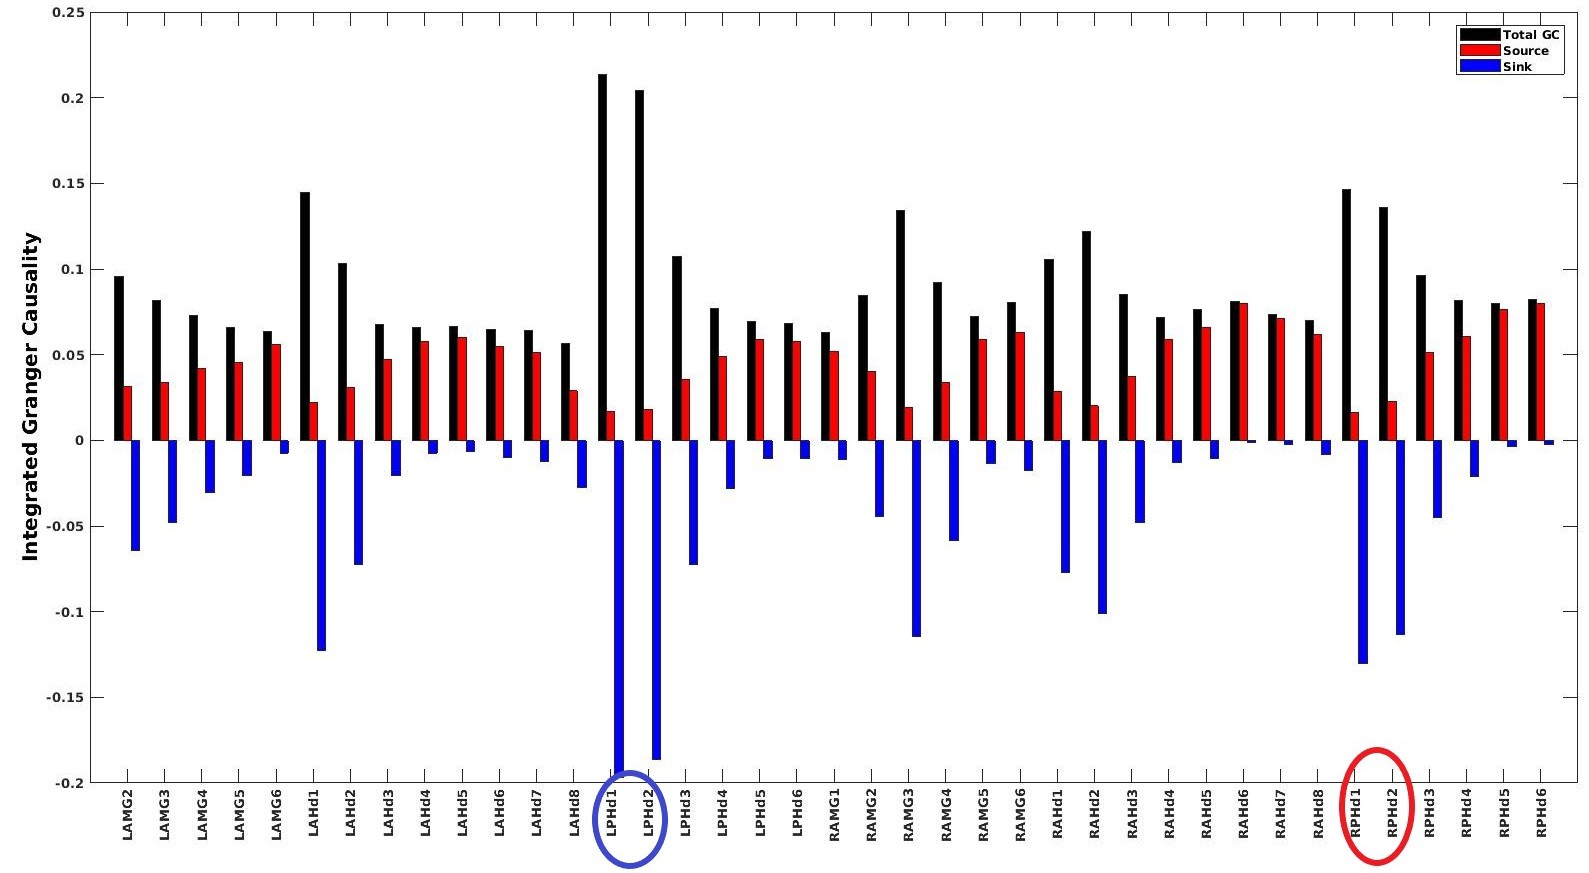
\includegraphics[height =3.5in]{Plots/Patient_A_preictal_high.jpg}
	}

	\caption{Patient A - Integrated Granger causality in the preictal state for high frequency activities}

	\label{fig:apdx_patient_a_preictal_high}
\end{figure*}


\begin{sidewaysfigure*}
\centerline{
	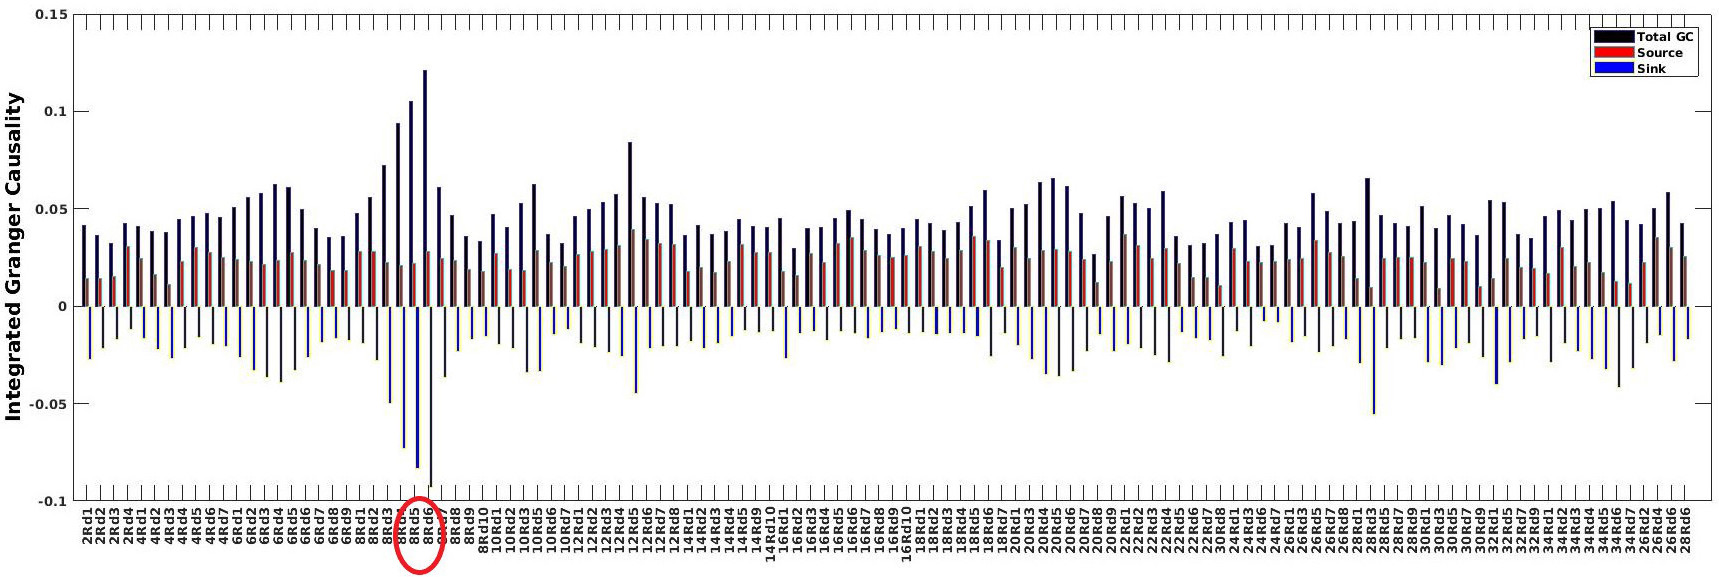
\includegraphics[height =2.8in]{Plots/Patient_B_preictal_high.jpg}
	}

	\caption{Patient B - Integrated Granger causality in the preictal state for high frequency activities}

	\label{fig:apdx_patient_b_preictal_high}
\end{sidewaysfigure*}

\begin{sidewaysfigure*}
\centerline{
	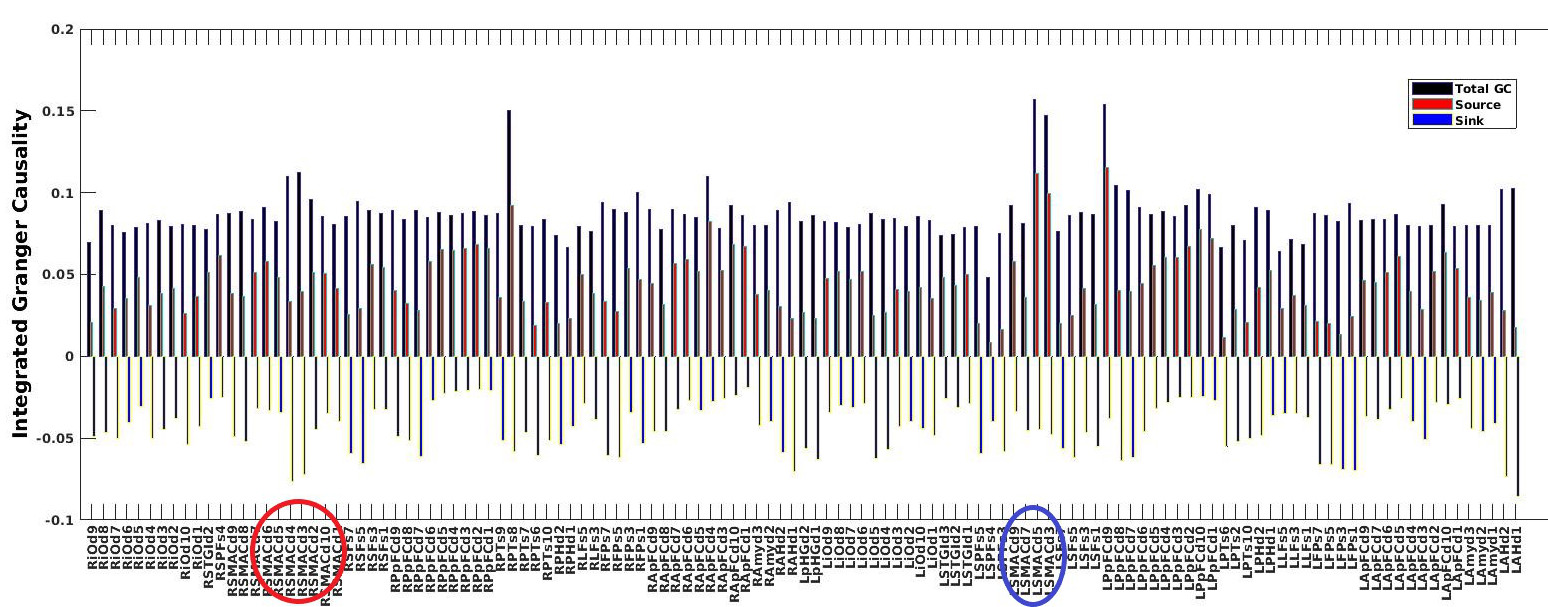
\includegraphics[height =3.2in]{Plots/Patient_C_preictal_high.jpg}
	}

	\caption{Patient C - Integrated Granger causality in the preictal state for high frequency activities}

	\label{fig:apdx_patient_c_preictal_high}
\end{sidewaysfigure*}


%\section{Granger causality on preictal infraslow}

\begin{figure*}
\centerline{
	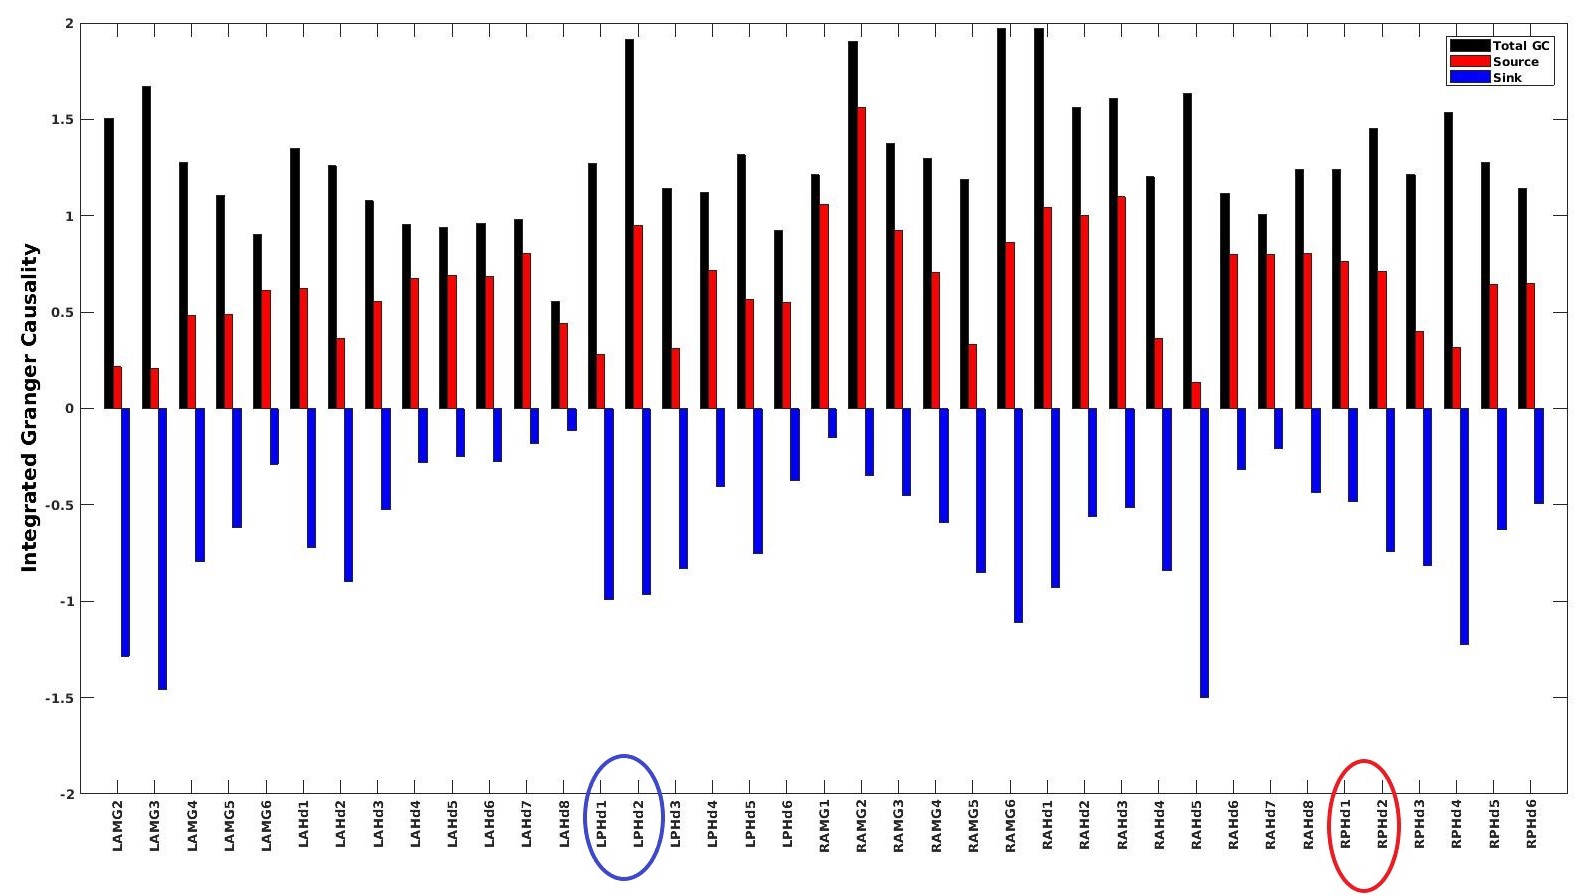
\includegraphics[height =3.5in]{Plots/Patient_A_preictal_low.jpg}
	}

	\caption{Patient A -  Integrated Granger causality in the preictal state for infraslow activities}

	\label{fig:apdx_patient_a_preictal_low}
\end{figure*}


\begin{sidewaysfigure*}
\centerline{
	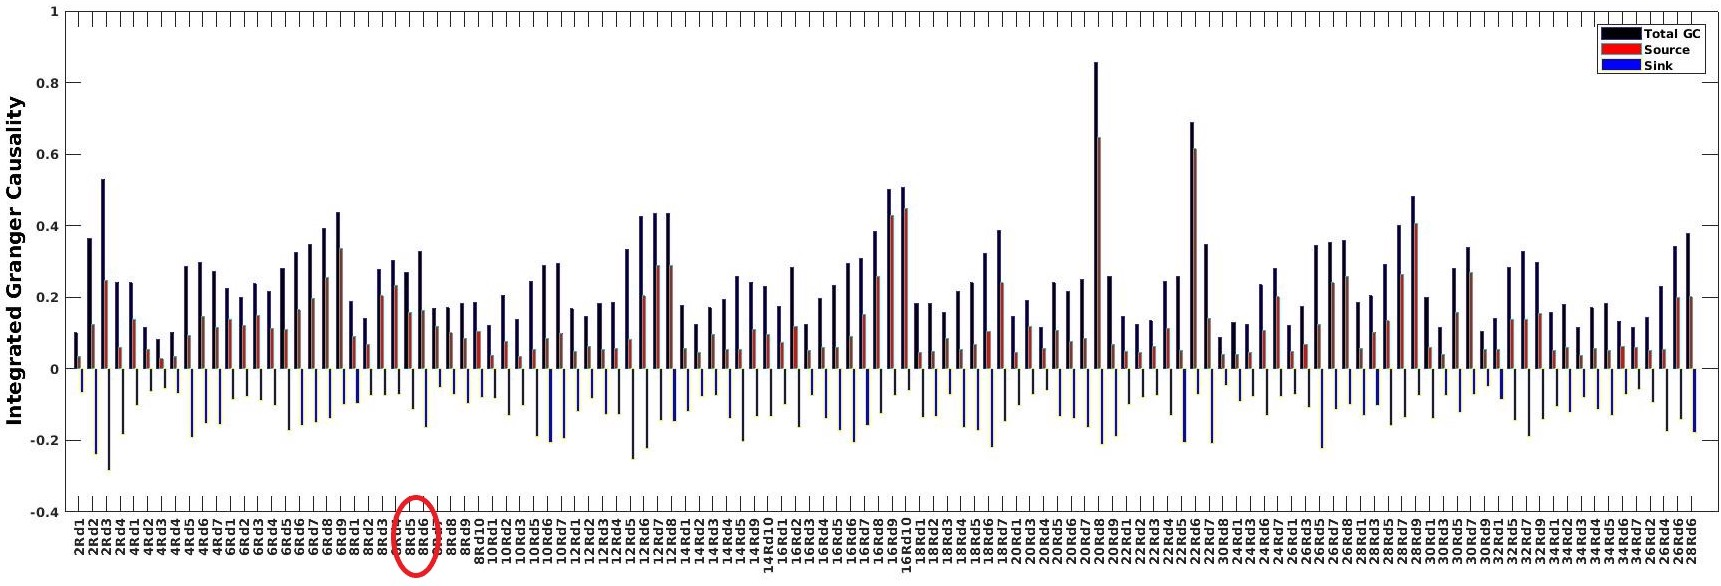
\includegraphics[height =2.8in]{Plots/Patient_B_preictal_low.jpg}
	}

	\caption{Patient B - Integrated Granger causality in the preictal state for infraslow activities}

	\label{fig:apdx_patient_b_preictal_low}
\end{sidewaysfigure*}


\begin{sidewaysfigure*}
\centerline{
	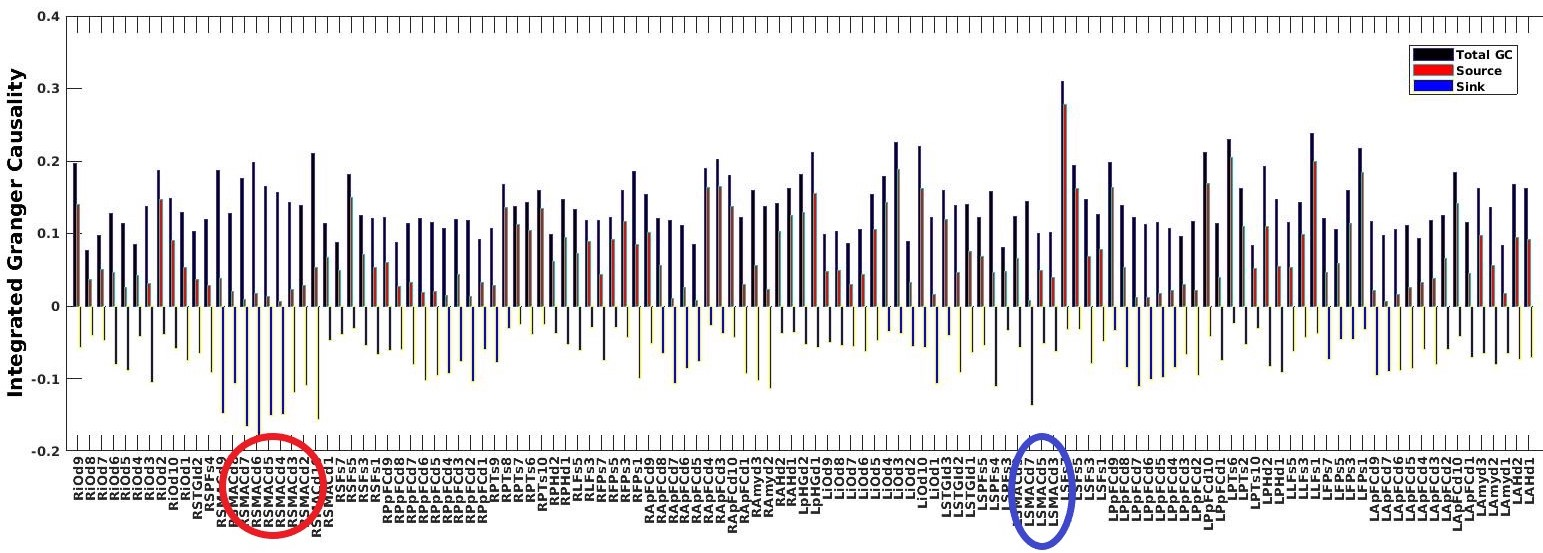
\includegraphics[height =3in]{Plots/Patient_C_preictal_low.jpg}
	}

	\caption{Patient C - Integrated Granger causality in the preictal state for infraslow activities}

	\label{fig:apdx_patient_c_preictal_low}
\end{sidewaysfigure*}


%\section{Granger causality on interictal high frequency}

\begin{figure*}
\centerline{
	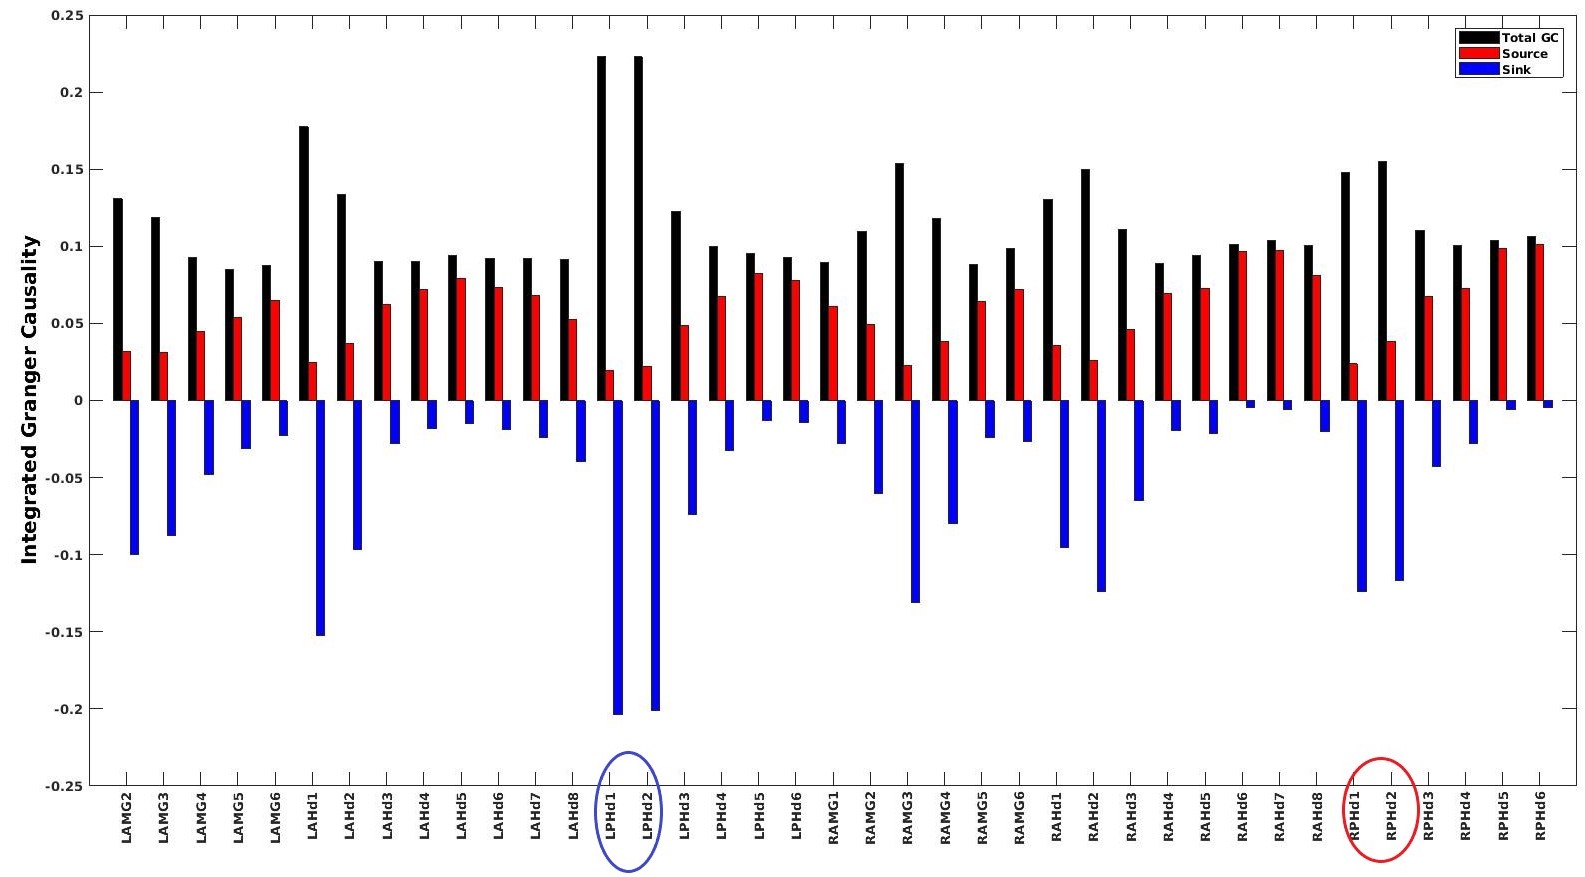
\includegraphics[height =3.5in]{Plots/Patient_A_interictal_high.jpg}
	}

	\caption{Patient A - Integrated Granger causality in the interictal state for high frequency activities}

	\label{fig:apdx_patient_a_interictal_high}
\end{figure*}


\begin{sidewaysfigure*}
\centerline{
	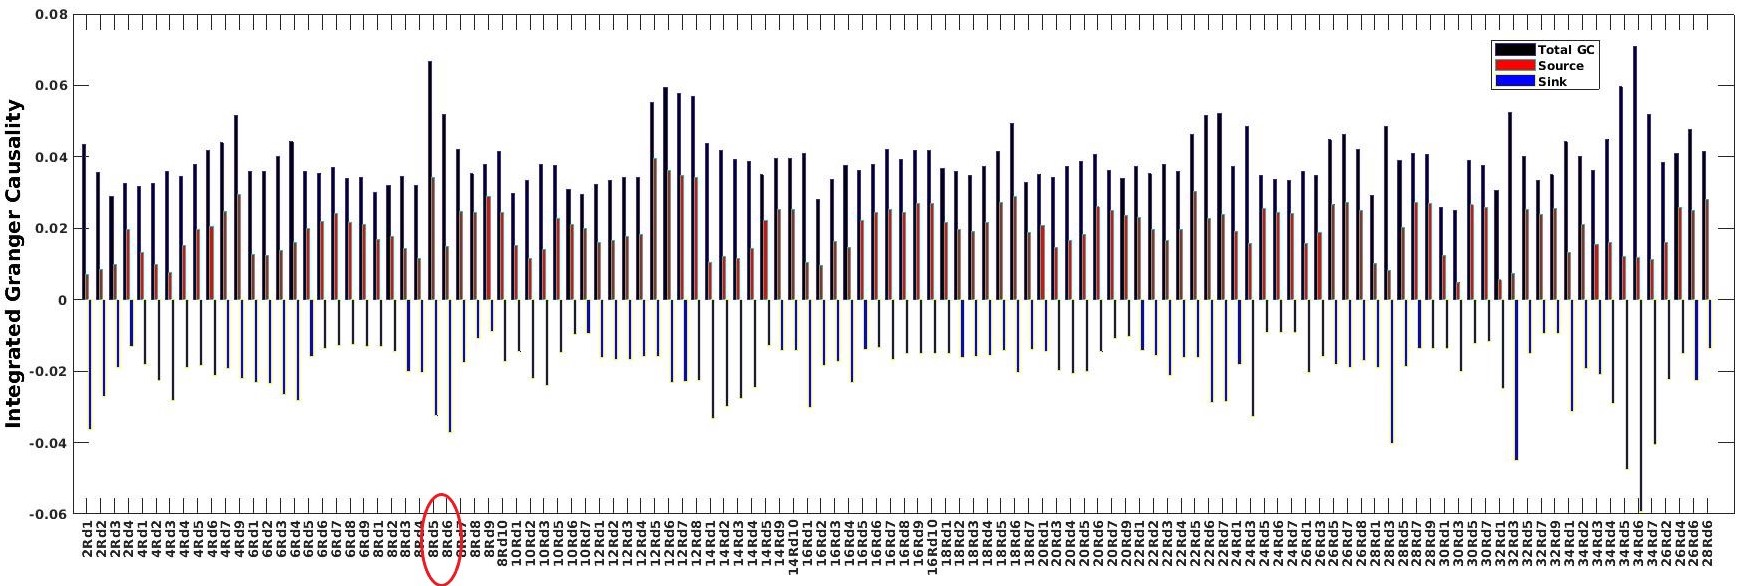
\includegraphics[height =2.8in]{Plots/Patient_B_interictal_high.jpg}
	}

	\caption{Patient B - Integrated Granger causality in the interictal state for high frequency activities}

	\label{fig:apdx_patient_b_interictal_high}
\end{sidewaysfigure*}

\begin{sidewaysfigure*}
\centerline{
	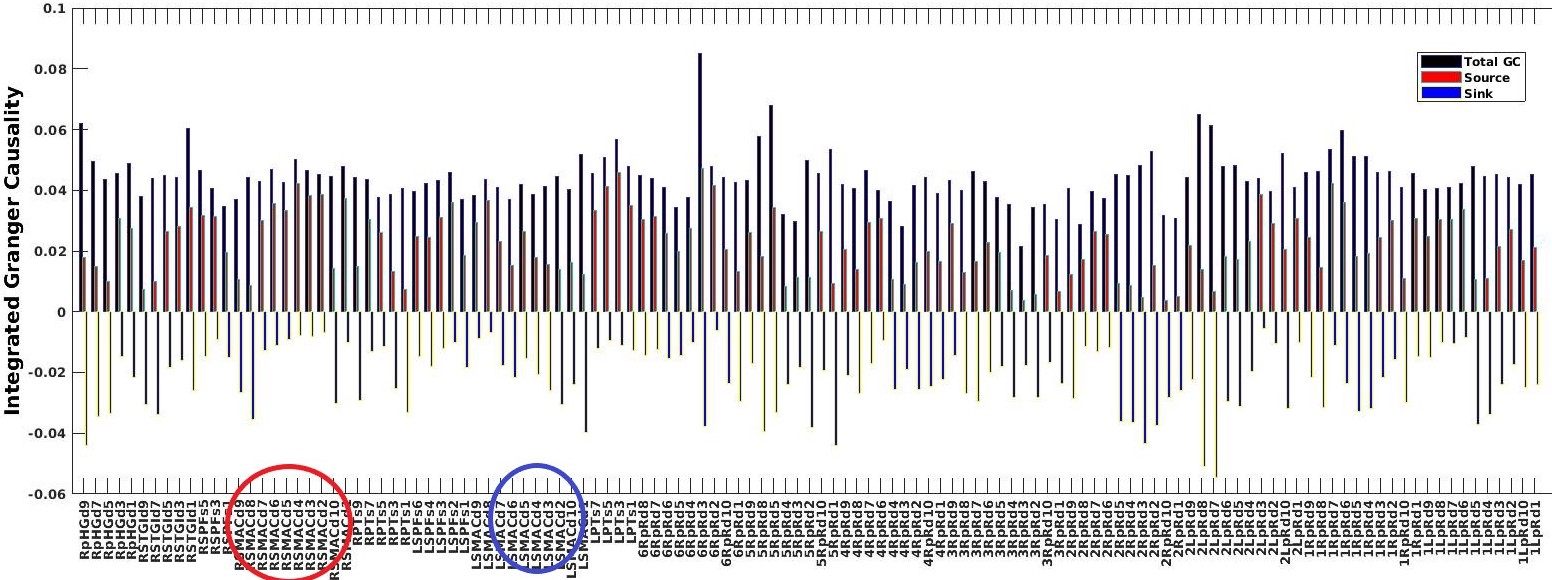
\includegraphics[height =3.1in]{Plots/Patient_C_interictal_high.jpg}
	}

	\caption{Patient C - Integrated Granger causality in the interictal state for high frequency activities}

	\label{fig:apdx_patient_c_interictal_high}
\end{sidewaysfigure*}



%\section{Granger causality on interictal infraslow}

\begin{figure*}
\centerline{
	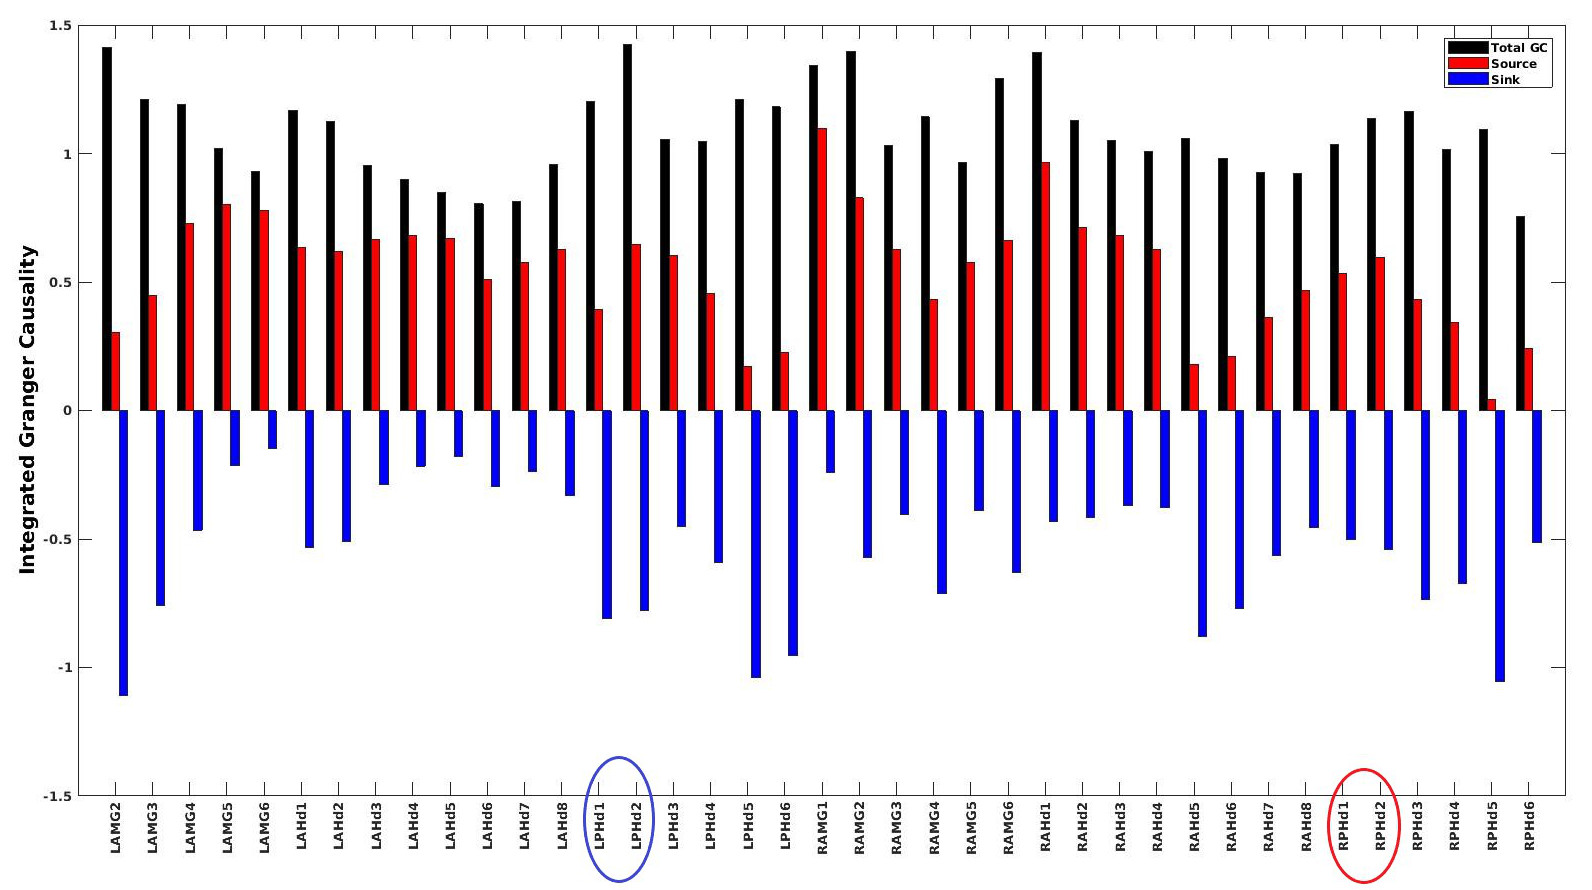
\includegraphics[height =3.5in]{Plots/Patient_A_interictal_low.jpg}
	}

	\caption{Patient A - Integrated Granger causality in the interictal state for infraslow activities}

	\label{fig:apdx_patient_a_interictal_low}
\end{figure*}

\begin{sidewaysfigure*}
\centerline{
	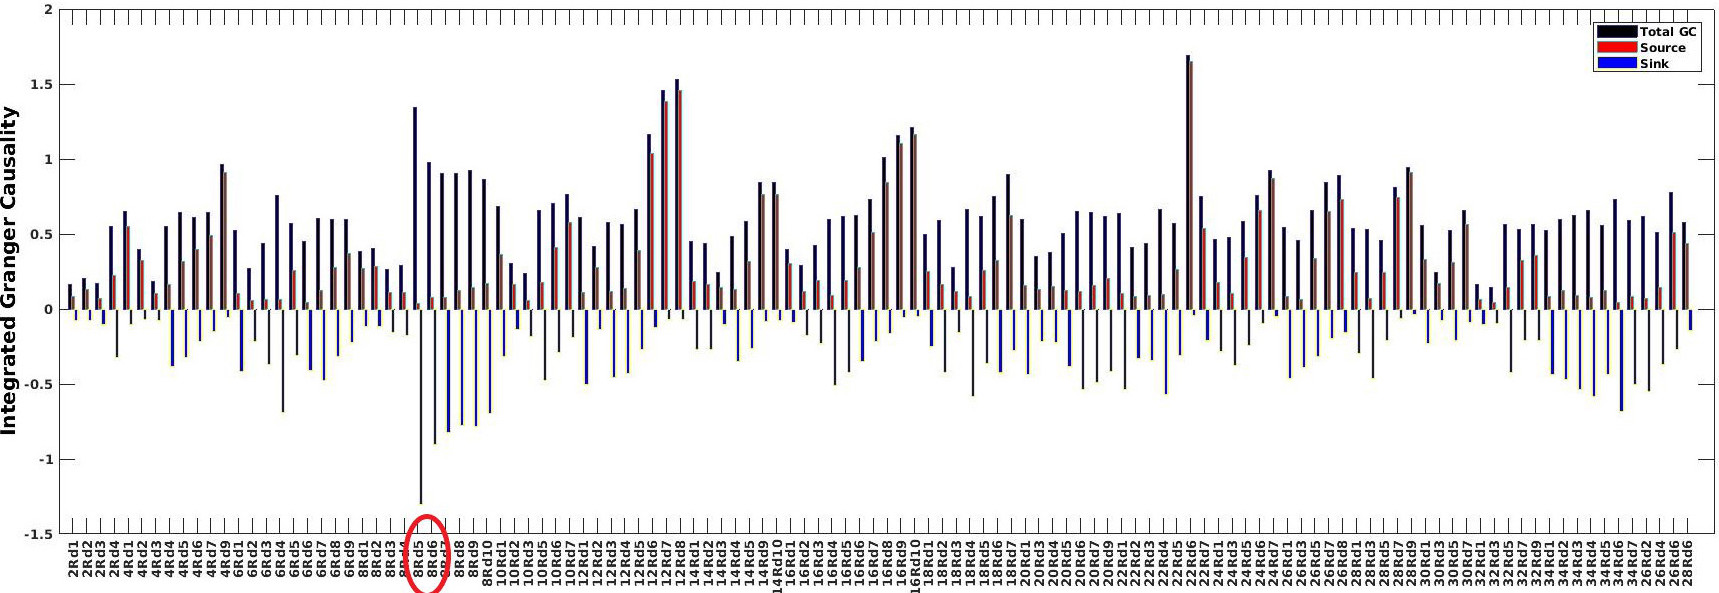
\includegraphics[height =2.8in]{Plots/Patient_B_interictal_low.jpg}
	}

	\caption{Patient B - Integrated Granger causality in the interictal state for infraslow activities}

	\label{fig:apdx_patient_b_interictal_low}
\end{sidewaysfigure*}


\begin{sidewaysfigure*}
\centerline{
	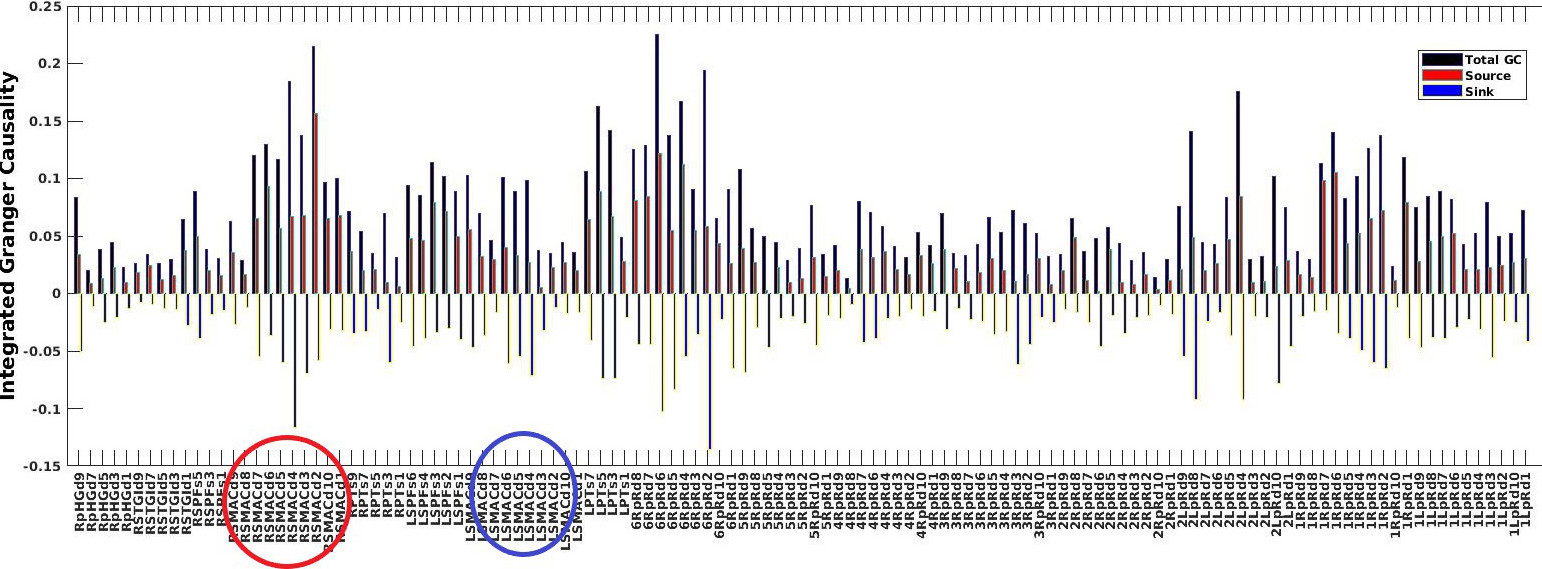
\includegraphics[height =3in]{Plots/Patient_C_interictal_low.jpg}
	}

	\caption{Patient C - Integrated Granger causality in the interictal state for infraslow activities}

	\label{fig:apdx_patient_c_interictal_low}
\end{sidewaysfigure*}
\chapter{Electrodes and corresponding MNI coordinates}

\section{MNI coordinates}
The table presented here shows the electrodes and their corresponding Montreal Neurological Institute (MNI) coordinates in MRI. MNI coordinates are a system standard coordinates for indexing the voxels within a volume of MRI or CT.

\begin{table}
\centering
\renewcommand{\arraystretch}{1.3} % Default value: 1
\setlength{\tabcolsep}{15pt} % Default value: 6pt
\begin{tabular}{|l|l|l|l|}
\hline
\textbf{Electrode} & \textbf{MNI (X, Y, Z)}  & \textbf{Electrode} & \textbf{MNI (X, Y, Z)}  \\ 
\hline
RSMAcd1   & (7, 2, 29)     & LSMAcd1   & (-5, 2, 31)   \\ \hline
RSMAcd2   & (9, 0, 34)     & LSMAcd2   & (-6, 2, 38)   \\ \hline
RSMAcd3   & (9, -1, 38)    & LSMAcd3   & (-7, 3, 42)   \\ \hline
RSMAcd4   & (12, -3, 44)   & LSMAcd4   & (-9, 2, 49)   \\ \hline
RSMAcd5   & (13, -4, 48)   & LSMAcd5   & (-10, 2, 53)  \\ \hline
RSMAcd6   & (15, -5, 53)   & LSMAcd6   & (-12, 3, 59)  \\ \hline
RSMAcd7   & (16, -6, 57)   & LSMAcd7   & (-13, 2, 63)  \\ \hline
RSMAcd8   & (19, -7, 62)   & LSMAcd8   & (-15, 1, 70)  \\ \hline
RSMAcd9   & (21, -9, 65)   & LSMAcd9   & (-16, 2, 73)  \\ \hline
RSMAcd10  & (22, -9, 68)   & LSMAcd10  & (-17, 1, 76)  \\ \hline
RpHGd1    & (20, -19, -28) & 5Rprd1    & (-1, 13, 25)  \\ \hline
RpHGd3    & (29, -16, -32) & 5Rprd2    & (-3, 12, 31)  \\ \hline
RpHGd7    & (48, -10, -31) & 5Rprd3    & (-6, 12, 36)  \\ \hline
RpHGd9    & (56, -7, -31)  & 5Rprd4    & (-8, 12, 40)  \\ \hline
RpHGd10   & (62, -7, -32)  & 5Rprd8    & (-20, 10, 58) \\ \hline
RSTGId1   & (46, 7, 5)     & 5Rprd9    & (-24, 8, 63)  \\ \hline
RSTGId3   & (55, 3, -5)    & 5Rprd10   & (-27, 8, 68)  \\ \hline
RSTGId5   & (62, 2, 5)     &           &               \\ \hline
\end{tabular}
\caption{MNI coordinates  for the iEEG electrodes and the corresponding voxels}

\label{table:channel_mni_coordinates_map}
\end{table}
\include{./Chapters/Appendix_D}
\include{./Chapters/Appendix_E}




%%%%%%%%%%%%%%%%%%%%%%%%%%%%%%%%%%%%%%%%%%%%%%%%%%%%%%%%%%%%%%%%%%%%%%
%               The dissertation ends here.                          %
%%%%%%%%%%%%%%%%%%%%%%%%%%%%%%%%%%%%%%%%%%%%%%%%%%%%%%%%%%%%%%%%%%%%%%

\end{document}
